\documentclass{amsart}

\usepackage[T1]{fontenc}
\usepackage{enumerate, amsmath, amsfonts, amssymb, amsthm, mathrsfs, wasysym, graphics, graphicx, xcolor, url, hyperref, hypcap, shuffle, xargs, multicol, overpic, pdflscape, multirow, hvfloat, minibox, accents, array, multido, xifthen, a4wide, ae, aecompl, blkarray, pifont, mathtools, etoolbox, dsfont, verbatim, stackrel, stmaryrd}
\usepackage{marginnote}
\hypersetup{colorlinks=true, citecolor=darkblue, linkcolor=darkblue}
\usepackage[all]{xy}
\usepackage[bottom]{footmisc}
\usepackage{tikz}
%\usepackage{tkz-graph}
%\usepackage{tikz-qtree}
\usetikzlibrary{trees, decorations, decorations.markings, shapes, arrows, matrix, calc, fit, intersections, patterns, angles, cd}
\usepackage[external]{forest}
%\tikzexternalize
\graphicspath{{figures/}{figures/nodes/}}
\makeatletter\def\input@path{{figures/}}\makeatother
\usepackage{caption}
\captionsetup{width=\textwidth}
\renewcommand{\topfraction}{1} % possibility to have one page of pictures
\renewcommand{\bottomfraction}{1} % possibility to have one page of pictures
\usepackage[noabbrev,capitalise]{cleveref}
\usepackage[export]{adjustbox}
\usepackage{ulem}\normalem

%%%%%%%%%%%%%%%%%%%%%%%%%%%%%%%%%%%%%%

% theorems
\newtheorem{theorem}{Theorem}%[section]
\newtheorem{corollary}[theorem]{Corollary}
\newtheorem{proposition}[theorem]{Proposition}
\newtheorem{lemma}[theorem]{Lemma}
\newtheorem{conjecture}[theorem]{Conjecture}
\newtheorem*{theorem*}{Theorem}%[section]

\theoremstyle{definition}
\newtheorem{definition}[theorem]{Definition}
\newtheorem{example}[theorem]{Example}
\newtheorem{remark}[theorem]{Remark}
\newtheorem{question}[theorem]{Question}
\newtheorem{problem}[theorem]{Problem}
\newtheorem{notation}[theorem]{Notation}
\newtheorem{assumption}[theorem]{Assumption}
\crefname{notation}{Notation}{Notations}
\crefname{problem}{Problem}{Problems}

% math special letters
\newcommand{\R}{\mathbb{R}} % reals
\newcommand{\N}{\mathbb{N}} % naturals
\newcommand{\Z}{\mathbb{Z}} % integers
\newcommand{\C}{\mathbb{C}} % complex
\newcommand{\I}{\mathbb{I}} % set of integers
\newcommand{\HH}{\mathbb{H}} % hyperplane
\newcommand{\K}{\mathbb{K}} % field
\newcommand{\fA}{\mathfrak{A}} % alternating group
\newcommand{\fB}{\mathfrak{S}^\textsc{b}} % signed symmetric group
\newcommand{\cA}{\mathcal{A}} % algebra
\newcommand{\cC}{\mathcal{C}} % collection
\newcommand{\cS}{\mathcal{S}} % ground set
\newcommand{\uR}{\underline{R}} % underline set
\newcommand{\uS}{\underline{S}} % underline set
\newcommand{\uT}{\underline{T}} % underline set
\newcommand{\oS}{\overline{S}} % overline set
\newcommand{\ucS}{\underline{\cS}} % underline ground set
\renewcommand{\c}[1]{\mathcal{#1}} % caligraphic letters
\renewcommand{\b}[1]{{\boldsymbol{#1}}} % bold letters
\newcommand{\bb}[1]{\mathbb{#1}} % bb letters
\newcommand{\f}[1]{\mathfrak{#1}} % frak letters
\newcommand{\h}{\widehat} % hat letters

% hello

% math commands
\newcommand{\set}[2]{\left\{ #1 \;\middle|\; #2 \right\}} % set notation
\newcommand{\bigset}[2]{\big\{ #1 \;\big|\; #2 \big\}} % big set notation
\newcommand{\Bigset}[2]{\Big\{ #1 \;\Big|\; #2 \Big\}} % Big set notation
\newcommand{\setangle}[2]{\left\langle #1 \;\middle|\; #2 \right\rangle} % set notation
\newcommand{\ssm}{\smallsetminus} % small set minus
\newcommand{\dotprod}[2]{\left\langle \, #1 \; \middle| \; #2 \, \right\rangle} % dot product
\newcommand{\symdif}{\,\triangle\,} % symmetric difference
\newcommand{\one}{\b{1}} % the all one vector
\newcommand{\eqdef}{\mbox{\,\raisebox{0.2ex}{\scriptsize\ensuremath{\mathrm:}}\ensuremath{=}\,}} % \eqdef
\newcommand{\defeq}{\mbox{~\ensuremath{=}\raisebox{0.2ex}{\scriptsize\ensuremath{\mathrm:}} }} % =:
\newcommand{\simplex}{\b{\triangle}} % simplex
\renewcommand{\implies}{\Rightarrow} % imply sign
\newcommand{\transpose}[1]{{#1}^t} % transpose matrix

% operators
\DeclareMathOperator{\conv}{conv} % convex hull
\DeclareMathOperator{\vect}{vect} % linear span
\DeclareMathOperator{\cone}{cone} % cone hull
\DeclareMathOperator{\inv}{inv} % inversions
\DeclareMathOperator{\ninv}{ninv} % inversions
\DeclareMathOperator{\Ima}{Im} % image
\DeclareMathOperator{\Vol}{Vol} % (mixed) volume

% others
\newcommand{\ie}{\textit{i.e.}~} % id est
\newcommand{\eg}{\textit{e.g.}~} % exempli gratia
\newcommand{\Eg}{\textit{E.g.}~} % exempli gratia
\newcommand{\apriori}{\textit{a priori}} % a priori
\newcommand{\viceversa}{\textit{vice versa}} % vice versa
\newcommand{\versus}{\textit{vs.}~} % versus
\newcommand{\aka}{\textit{a.k.a.}~} % also known as
\newcommand{\perse}{\textit{per se}} % per se
\newcommand{\ordinal}{\textsuperscript{th}} % th for ordinals
\newcommand{\ordinalst}{\textsuperscript{st}} % st for ordinals
\definecolor{darkblue}{rgb}{0,0,0.7} % darkblue color
\definecolor{green}{RGB}{57,181,74} % darkblue color
\definecolor{violet}{RGB}{147,39,143} % darkblue color
\newcommand{\darkblue}{\color{darkblue}} % darkblue command
\newcommand{\defn}[1]{\textsl{\darkblue #1}} % emphasis of a definition
\newcommand{\para}[1]{\smallskip\noindent\uline{#1.}} % paragraph
\renewcommand{\topfraction}{1} % possibility to have one page of pictures
\renewcommand{\bottomfraction}{1} % possibility to have one page of pictures
%\renewcommand\labelitemi{$\diamond$} % redefine itemize default symbol

% marginal comments
\usepackage{todonotes}
\newcommand{\vincent}[1]{\todo[color=blue!30]{\rm #1 \\ \hfill --- V.}}
\newcommand{\Vincent}[1]{\todo[inline, color=blue!30]{\rm #1 \\ \hfill --- V.}}
\newcommand{\jean}[2][]{\todo[size=\scriptsize, color=orange!30,#1]{\rm #2 \\ \hfill --- J.}}
\newcommand{\Jean}[2][]{\todo[inline, size=\scriptsize, color=orange!30,#1]{\rm #2 \\ \hfill --- J.}}

% lattices
\newcommand{\meet}{\wedge} % meet
\newcommand{\join}{\vee} % join
\newcommand{\bigMeet}{\bigwedge} % meet
\newcommand{\bigJoin}{\bigvee} % join
\newcommandx{\projDown}[1][1={}]{\smash{\pi_\downarrow^{#1}}} % down projection map
\newcommandx{\projUp}[1][1={}]{\smash{\pi^\uparrow_{#1}}} % up projection map
\newcommand{\con}{\mathrm{con}} % congruence

% geometry
\newcommandx{\Fan}[1][1=D]{\mathcal{F}_{#1}} % fan
\newcommand{\polytope}[1]{\mathds{#1}} % font polytope

% polytopes
\newcommand{\Perm}{\polytope{P}} % permutahedron
\newcommand{\Asso}{\polytope{A}} % associahedron
% rectangulotopes
\newcommand{\WRP}{\polytope{WR}} % weak rectangulotope
\newcommand{\SRP}{\polytope{SR}} % strong rectangulotope
% shard polytopes
\newcommand{\SP}{\polytope{SP}}

% horizontal pattern
\newcommand{\horizontalPattern}{\smash{\raisebox{-.15cm}{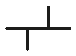
\includegraphics[scale=.5]{horizontalPattern}}}} 
% vertical pattern
\newcommand{\verticalPattern}{\smash{\raisebox{-.25cm}{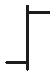
\includegraphics[scale=.5]{verticalPattern}}}} 

% Loday and anti-Loday accents (?)
\newcommand{\loday}[1]{\smash{\overset{\frown}{#1}}}
\newcommand{\antiloday}[1]{\smash{\overset{\smile}{#1}}}
% yin and yang accents (?)
\newcommand{\yang}[1]{\smash{\overset{\backsim}{#1}}}
\newcommand{\yin}[1]{\smash{\overset{\sim}{#1}}}
% weak and strong equivalence on S_n
\newcommand{\baxtereq}{\asymp}%{\stackrel{\frown}{\smile}}
\newcommand{\strongeq}{\simeq}% % J: I would like to stack \backsim and \sim instead

% formating the table of contents
\setcounter{tocdepth}{4}
\makeatletter
\def\l@part{\@tocline{1}{8pt}{0pc}{}{}}
\def\l@section{\@tocline{1}{4pt}{0pc}{}{}}
\makeatother
\let\oldtocpart=\tocpart
\renewcommand{\tocpart}[2]{\sc\large\oldtocpart{#1}{#2}}
\let\oldtocsection=\tocsection
\renewcommand{\tocsection}[2]{\bf\oldtocsection{#1}{#2}}
\let\oldtocsubsubsection=\tocsubsubsection
\renewcommand{\tocsubsubsection}[2]{\quad\oldtocsubsubsection{#1}{#2}}

%%%%%%%%%%%%%%%%%%%%%%%%%%%%%%%%%%%%%%

%\title{Rectangulation polytopes}
\title{Rectangulotopes}

\thanks{VP was partially supported by the Spanish grant PID2022-137283NB-C21 of MCIN/AEI/10.13039/501100011033 / FEDER, UE, by Departament de Recerca i Universitats de la Generalitat de Catalunya (2021 SGR 00697), by the French grant CHARMS (ANR-19-CE40-0017), and by the French--Austrian projects PAGCAP (ANR-21-CE48-0020 \& FWF I 5788).}

\author{Jean Cardinal}
\address{Université libre de Bruxelles (ULB)}
\email{jean.cardinal@ulb.be}
\urladdr{\url{https://jean.cardinal.web.ulb.be}}

\author{Vincent Pilaud}
\address{Universitat de Barcelona}
\email{vincent.pilaud@ub.edu}
\urladdr{\url{https://www.ub.edu/comb/vincentpilaud/}}

%%%%%%%%%%%%%%%%%%%%%%%%%%%%%%%%%%%%%%

\begin{document}

\begin{abstract}
  Rectangulations are decompositions of a square into finitely many axis-aligned rectangles.
  We describe realizations of $(n-1)$-dimensional polytopes associated with rectangulations composed of $n$ rectangles.
  They are defined as quotientopes of natural congruence relations on the weak Bruhat order on permutations in $\f{S}_n$, and their skeleta are flip graphs on rectangulations.
  We give a thorough description of geometric realizations of these polytopes, including elementary formulas for computing the coordinates of each vertex of the polytope, in the spirit of Loday's realization of the associahedron.
\end{abstract}

\maketitle

\tableofcontents

%%%%%%%%%%%%%%%%%%%%%%%%%%%%%%%%%%%%%%

\section{Introduction}

\subsection{Polytopes of permutations, triangulations, and rectangulations}

The encoding of combinatorial objects in the form of a polyhedral structure is a recurrent theme in geometric and algebraic combinatorics.
An elementary yet striking example of this idea is the \defn{permutahedron} $\Perm (n)$, defined as the convex hull of the points $\sum_{i\in [n]} \pi^{-1}(i)\cdot \mathbf{e}_i$, for all permutations $\pi\in\f{S}_n$.
It is an $(n-1)$-dimensional polytope, whose facets are indexed by the proper nonempty subsets of $[n]$, and whose skeleton is the Cayley graph of the symmetric group for the generators consisting of adjacent transpositions.
The many generalizations and extensions of the permutahedra gave rise to a flourishing theory of \defn{generalized permutahedra}~\cite{Postnikov} (or \defn{deformed permutahedra}).

Among those, the \defn{associahedron} is a classical, ubiquitous polytope, first defined by Tamari~\cite{T51}, then studied by Stasheff in a topological context~\cite{S63}, that has since then found applications in various areas of mathematics, including topology, operads, cluster algebras, combinatorial Hopf algebras, and physics~\cite{MR4675114}.
It was first defined as a combinatorial object, before various families of geometric realizations were shown to exist~\cite{MR1022776,MR1941227,MR2108555,MR3437894}.
The face lattice of the $(n-1)$-dimensional associahedron is the reverse inclusion poset of nonintersecting diagonals of a convex $(n+3)$-gon.
In particular, it skeleton is the \defn{flip graph} on \defn{triangulations} of the $(n+3)$-gon, or equivalently -- via a standard Catalan bijection -- the \defn{rotation graph} on \defn{binary trees} with $n$ internal nodes, the structure of which has been the subject of many investigations, with applications in computer science~\cite{MR928904,MR3197650}.
In 2004, Loday published the following elegant realization of the associahedron~\cite{MR2108555}, giving a recipe for computing the coordinates of a vertex given the corresponding binary tree.

\begin{theorem}
  \label{thm:loday}
  The $(n-1)$-dimensional associahedron is realized by the convex hull~$\Asso (n)$ of the points
  $\sum_{i\in [n]} w^T_i \cdot \mathbf{e}_i$ for all binary trees $T$ on $n$ internal nodes, with
  \[
  w^T_i \eqdef \ell^T_i\cdot r^T_i,
  \]
  where $\ell^T_i$ and $r^T_i$ respectively denote the number of leaves in the left and right subtrees of $i$ in $T$.
\end{theorem}

A natural object associated with the associahedron is the \defn{Tamari lattice}, the cover graph of which is isomorphic to the skeleton of the associahedron.
The Tamari lattice is known to be the quotient of the weak Bruhat order by a \defn{lattice congruence} relation called the \defn{sylvester congruence}.
Pilaud and Santos~\cite{MR3964495}, answering a question of Reading~\cite{MR2142177}, proved that with \emph{every} lattice congruence of the weak Bruhat order, one can associate a polytope whose skeleton is the cover graph of the lattice quotient, and more precisely whose normal fan is the \defn{quotient fan} defined by gluing the cones of the \defn{braid fan} (the type $A$ Coxeter arrangement) that belong to the same congruence class.
Those polytopes are generalized permutahedra that they called \defn{quotientopes}.
Associahedra are therefore the quotientopes of a congruence of the weak Bruhat order whose classes are in bijection with triangulations.

The goal of this paper is to describe the quotientopes of congruences of the weak Bruhat order whose classes are in bijection with (equivalence classes of) \defn{rectangulations}, defined as decompositions of a square into finitely many axis-aligned rectangles.
The combinatorics of rectangulations has been studied for decades~\cite{MR2233287,MR2871762,MR2864445,MR2763051,MR3084577,MR3878132,MR4598046}, and the order-theoretic take on these structures has already proved useful.
%, in particular in the context of electronic engineering applications~\cite{}.

The relevant lattice congruences are the \defn{weak rectangulation congruence} (or \defn{Baxter congruence}) on one hand, studied by Law and Reading~\cite{MR2871762}, and whose classes are one-to-one with \defn{weak rectangulations} (or \defn{diagonal rectangulations}) and \defn{Baxter permutations}, and the \defn{strong rectangulation congruence}, whose classes are in bijection with \defn{strong rectangulations}~\cite{MR2864445}.
The latter is mentioned by Reading~\cite{MR3335492} (see for instance in Theorem 1.2, and Example 4.11), and studied more recently by Asinowski, Cardinal, Felsner, and Fusy~\cite{ACFF24}.

One of our main results is an elementary description of the vertex coordinates of a realization of both families of quotientopes, in the spirit of Loday's realization in Theorem~\ref{thm:loday}.
The quotientopes corresponding to the weak rectangulation congruence will be referred to as the \defn{weak rectangulotopes} and denoted by $\WRP(n)$.
The skeleton of $\WRP(n)$ is isomorphic to the flip graph of weak rectangulations of size $n$ defined by Law and Reading~\cite{MR2871762}.
Similarly, the quotientopes corresponding to the strong rectangulation congruence will be called the \defn{strong rectangulotopes} and denoted by $\SRP(n)$.
The skeleton of $\SRP(n)$ is isomorphic to the flip graph of strong rectangulations of size $n$ defined by Meehan~\cite{MR3697823} (see also~\cite{ACFF24}).

Rectangulotopes enrich the family of natural quotientopes, alongside associahedra and permutreehedra~\cite{MR3856522}, and are instructive examples of application of the theory of lattice congruences to concrete combinatorial objects.

% jean:{Vincent, you may want to say more about permutreehedra, incl. the Loday coordinates.}

\subsection{Weak and strong rectangulations}

We give the necessary definitions for stating our results on the vertex description of the weak and strong rectangulotopes.

\begin{itemize}
\item Terminology: rectangles, \defn{vertices}, \defn{segments}, \defn{generic} rectangulation
\item \defn{Wall slides}
\item Two equivalence classes: \defn{weak equivalence} preserving rectangle-segment adjacencies, and \defn{strong equivalence} preserving rectangle-rectangle adjacencies.
\item Weak equivalence classes have a \defn{diagonal} representative.
\item \defn{Flip graphs} on rectangulations
\end{itemize}


\subsection{Source and target trees of a rectangulation}
\label{subsec:sourceTargetTrees}

% jean:{Here only give the definitions allowing to state the results.}

\begin{figure}
	\centerline{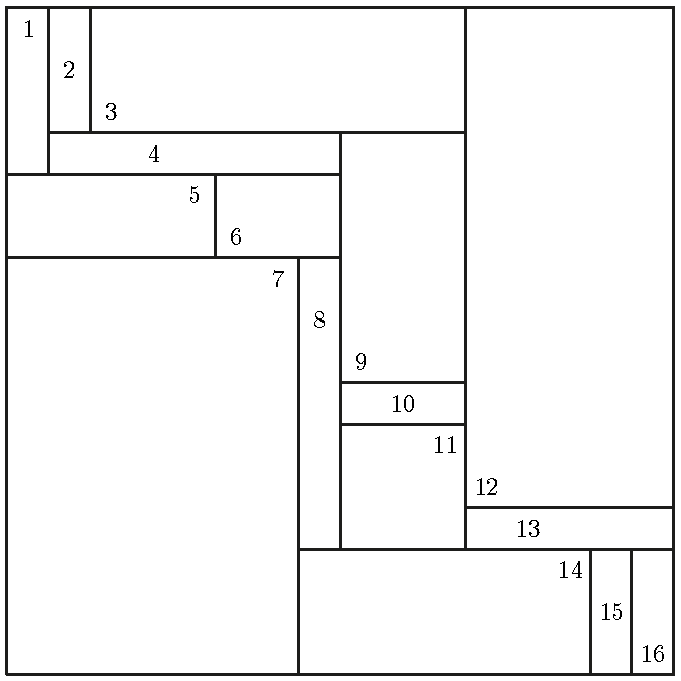
\includegraphics[width=.5\textwidth]{weakRectangulation} \qquad 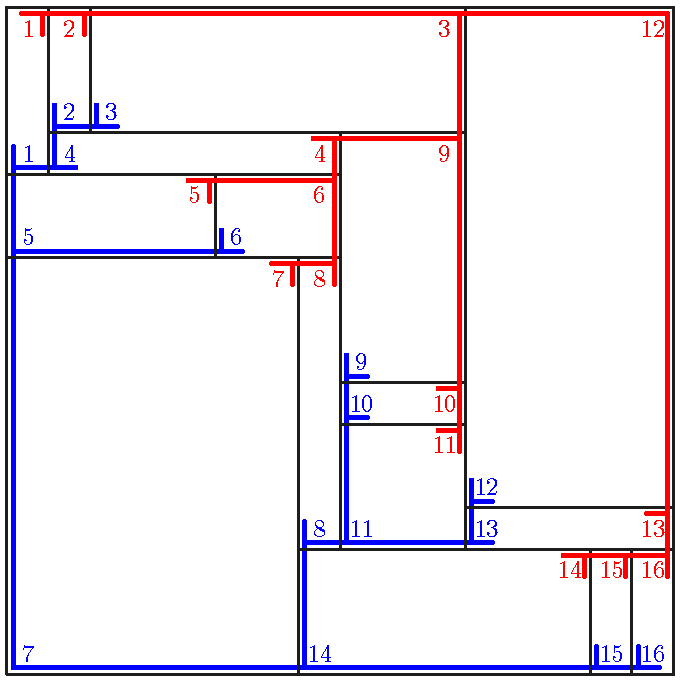
\includegraphics[width=.5\textwidth]{weakRectangulationTrees}}
	\caption{A weak rectangulation (left) and its pair of separated twin trees (right). Example from \cite{ACFF24}.}
	% The corresponding twisted Baxter permutation is $[7, 5, 1, 14, 8, 6, 4, 2, 11, 10, 9, 3, 15, 16, 13, 12]$ and its inverse is $[3, 8, 12, 7, 2, 6, 1, 5, 11, 10, 9, 16, 15, 4, 13, 14]$.
	\label{fig:weakRectangulation}
\end{figure}

\begin{figure}
	\centerline{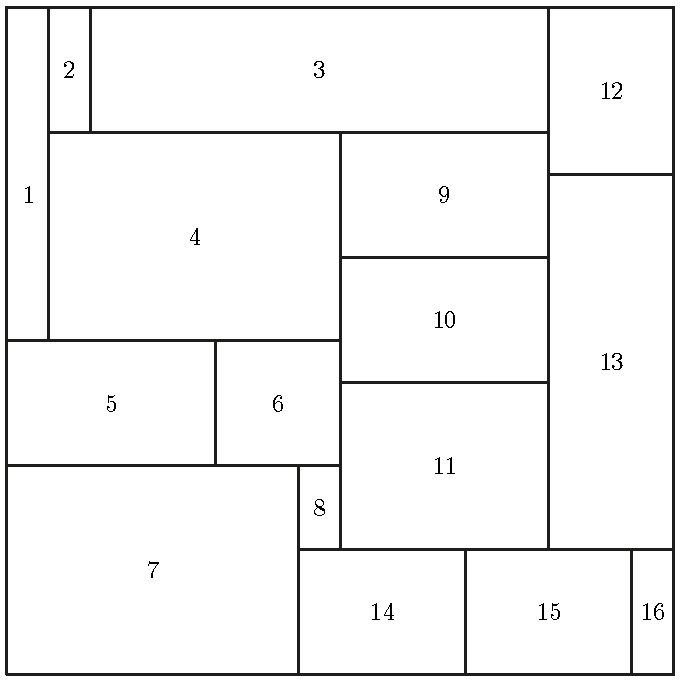
\includegraphics[width=.5\textwidth]{strongRectangulation} \qquad 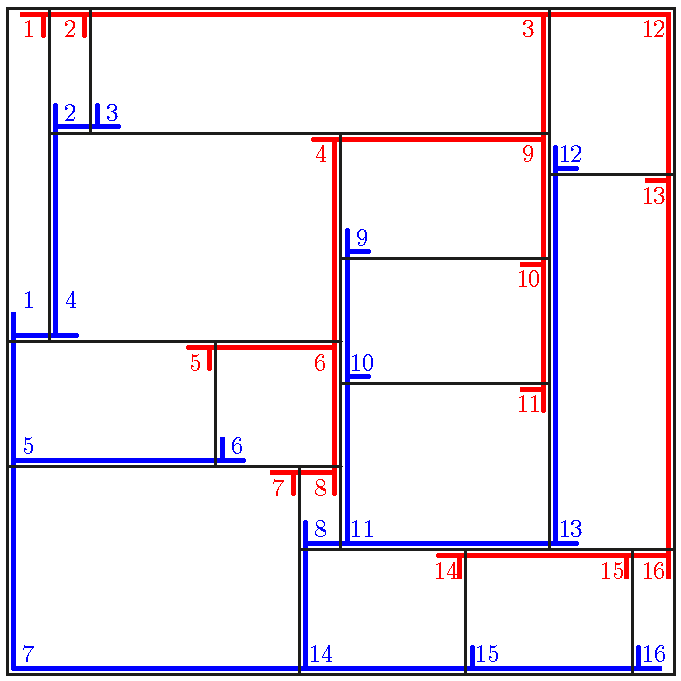
\includegraphics[width=.5\textwidth]{strongRectangulationTrees}}
	\caption{A strong rectangulation (left) and its pair of intertwining binary trees (right). Example from \cite{ACFF24}.}
        % The corresponding $2$-clumped permutation is $[7,5,14,8,1,6,15,11,4,10,16,2,9,13,3,12]$ and its inverse is $[5, 12, 15, 9, 2, 6, 1, 4, 13, 10, 8, 16, 14, 3, 7, 11]$.
        \label{fig:strongRectangulation}
\end{figure}

Fix a rectangulation~$R$ with $n$ rectangles, and consider the directed graph~$D(R)$ whose vertex set is the set of all vertices of~$R$, and whose edges are obtained as follows.
For each rectangle~$r$ of~$R$, we include in~$D(R)$ four edges joining the vertices of~$r$, where the horizontal edges are oriented from left to right, and the vertical edges are oriented from bottom to top.
Hence, the bottom left corner of~$r$ is its source~$s(r)$, while its top right corner is its target~$t(r)$.
Note that since~$R$ is generic, the sources~$\set{s(r)}{r \in [n]}$ and the targets~$\set{t(r)}{r \in [n]}$ are disjoint.
The \defn{source tree}~$S(R)$ (resp.~\defn{target tree}~$T(R)$) is the subgraph of~$D(R)$ induced by the sources~$\set{s(r)}{r \in [n]}$ (resp.~by the targets~$\set{t(r)}{r \in [n]}$).
See \cref{fig:strongRectangulation}.

\begin{lemma}
The source tree~$S(R)$ (resp.~target tree~$T(R)$) is a binary tree, rooted at the bottom left (resp.~top right) corner of~$R$, and oriented from (resp.~towards) its root.
\end{lemma}

\begin{comment}
\begin{proof}
By symmetry, we only prove the statement for the source tree~$S(R)$.
As the rectangulation is generic, each source~$s(r)$ distinct from the bottom left corner of~$R$ is either on the top edge of a rectangle~$r'$ or on the right edge of a rectangle~$r'$ (but not both).
This shows that~$r$ distinct from the bottom left rectangle of~$R$ has a unique parent~$r'$ in~$S(R)$, so that~$S(R)$ is indeed a tree on~$[n]$.
This tree is binary as each node has at most one vertical child and one horizontal child, and no other children.
\end{proof}
\end{comment}

We complete each node of~$S(R)$ and~$T(R)$ with a vertical (resp.~horizontal) leaf if it has no vertical (resp.~horizontal) child, see \cref{fig:strongRectangulation}.
Recall that the \defn{inorder labeling} of a binary tree~$T$ is the labeling of the nodes of~$T$ such that the label of each node~$t$ of~$T$ is larger than all labels in the left subtree of~$t$ and larger than all labels in the right subtree of~$t$.

\begin{lemma}
For any rectangle~$r$ of~$R$, the inorder label of the source~$s(r)$ in~$S(R)$ coincides with the inorder label of the target~$t(r)$ in~$T(R)$.
\end{lemma}

This enables to unambiguously label the rectangles of~$R$ by the inorder 
The resulting labeling coincides with the NW--SE labeling of~\cite{ACFF24}.
From now on, the labels of the rectangles in a rectangulations are the inorder labels, and the two trees $T(R)$ and $S(R)$ are defined on the vertex set $[n]$ accordingly.
For each $i\in [n]$, we refer to its two subtrees in $T(R)$ as the \defn{horizontal} and \defn{vertical subtrees}, and similarly for $S(R)$.

\subsection{Weak rectangulotopes}

Our first result is a concise formula for the coordinates of the vertices of the  weak rectangulotopes $\WRP(n)$, that consists of applying Loday's formula on each of the source and target trees of the rectangulation.
This materializes the result of Law and Reading that the weak rectangulotopes are Minkowski sums of two opposite associahedra~\cite{MR2871762}.

\begin{theorem}
  The $(n-1)$-dimensional weak rectangulotope is realized by the convex hull $\WRP (n)$ of the points
  $\sum_{i\in [n]} (\loday{w}^R_i - \antiloday{w}^R_i)\cdot \mathbf{e}_i$ for all weak rectangulations $R$ on $n$ rectangles,
  with
  \[
%  \begin{split}
%    \loday{w}^R_i \eqdef & h(T, i)\cdot v(T,i) \\
%    \antiloday{w}^R_i \eqdef & h(S, i)\cdot v(S,i),
%  \end{split}
    \loday{w}^R_i \eqdef h^T_i\cdot v^T_i
    \qquad\text{and}\qquad
    \antiloday{w}^R_i \eqdef h^S_i\cdot v^S_i,
  \]
  where~$S$ and~$T$ are the source and target trees of the rectangulation~$R$, and $h^T_i$ and $v^T_i$ denote the number of leaves in the horizontal and vertical subtrees of $i$ in~$T$.
\end{theorem}

\begin{example}
  The vertex of~$\WRP (16)$ corresponding to the weak rectangulation of \cref{fig:weakRectangulation} is
  \[
  (-3, 0, 26, 2, -9, 5, -69, -4, 17, 0, -8, 59, 2, -20, 0, 2).
  \]
  For instance, the $4$th coordinate is $h^T_4 \cdot v^T_4 - h^S_4 \cdot v^S_4 = 1 \cdot 5 - 1 \cdot 3 = 2$.
\end{example}

\subsection{Strong rectangulotopes}

In order to exhibit a similar realization for the strong rectangulotopes, we need to count subsets of leaves that lie in some subtrees of both the source and target trees of a rectangulation.
Two leaves of the trees $T(R)$ and $S(R)$ are said to be \defn{common leaves} if the edges to their parents lie on the same segment of $R$.
We denote by %$i|j$ and $\frac{\ j\ }i$
$i \, \backslash \, j$ the situation where the rectangle labeled $i$ touches the rectangle labeled $j$ either from the left or from below in $R$. %, respectively.

\begin{theorem}
  The $(n-1)$-dimensional strong rectangulotope is realized by the convex hull~$\SRP (n)$ of the points
  \[
  \sum_{i,j\in [n], i< j} (\yin{w}^R_{i,j} - \yang{w}^R_{i,j})\cdot (\mathbf{e}_i - \mathbf{e}_j),
  \]
   for all strong rectangulations $R$ on $n$ rectangles, with
  \[
%  \begin{split}
%    \yin{w}_{i,j} \eqdef & h(T, i) \cdot cv (T, S, i, j)\cdot h(S, j)\cdot \llbracket \neg i\backslash j \rrbracket \\% \text { if not } i\backslash j, \text{and } 0\text{ otherwise.} \\ % \neg i|j \text{ and } \neg \frac{\ j\ }i ] \\
%    \yang{w}_{i,j} \eqdef & v(S, i) \cdot ch (S, T, i, j)\cdot v(T, j) \cdot \llbracket \neg j\backslash i \rrbracket,
%  \end{split}
    \yin{w}^R_{i,j} \eqdef h^T_i \cdot cv^{T,S}_{i,j}\cdot h^S_ j\cdot \llbracket \neg \, i \, \backslash \, j \rrbracket
    \qquad\text{and}\qquad
    \yang{w}^R_{i,j} \eqdef v^S_i \cdot ch^{S,T}_{i,j}\cdot v^T_j \cdot \llbracket \neg \, j \, \backslash \, i \rrbracket,
  \]
 where:
  \begin{itemize}
  \item $S$ and $T$ are the source and target trees of the rectangulation~$R$,
  \item $h^T_i$ and $v^T_i$ denote the number of leaves in the horizontal and vertical subtrees of $i$ in~$T$,
  \item $ch^{T,S}_{i,j}$ (resp.~$cv^{T,S}_{i,j}$) denote the number of common leaves of the horizontal (resp.~vertical) subtree of $i$ in $T$ and the horizontal (resp.~vertical) subtree of $j$ in $S$.
  \end{itemize}
\end{theorem}

% jean:{Is there better way to write this down/compute? Here we do not take advantage of the fact that at most one of the two factors $\yin{w}_{i,j}$ and $\yang{w}_{i,j}$ is nonzero.}

\begin{example}
The vertex of~$\SRP (16)$ corresponding to the strong rectangulation of \cref{fig:strongRectangulation} is
\[
???
\]
For instance, the $4$th coordinate is $???$.

\end{example}

\subsection{Plan of the paper}

Section~\ref{sec:quotientopes} is dedicated to the background on quotientopes and their realizations as Minkowski sums of \defn{shard polytopes}, due to Padrol, Pilaud, and Ritter~\cite{MR4584712}, which will be our main tool throughout.
Section~\ref{sec:wr} details the case of weak rectangulations, while Section~\ref{sec:sr} deals with strong rectangulations.
In both cases, in addition to the vertex coordinates, we give the description of the face lattices and the submodular functions defining the polytopes.

\subsection*{Acknowledgments}

This work was initiated at the Workshop on Combinatorics, Algorithms, and Geometry organized by Torsten M\"utze on March 4-8, 2024 in Dresden, Germany.
The authors thank Namrata and Torsten M\"utze for the organization and the other participants of the workshop for the stimulating interactions, notably on other combinatorial aspects of rectangulations.

%%%%%%%%%%%%%%%%%%%%%%%%%%%%%%%%%%%%%%

\section{Quotientopes}
\label{sec:quotientopes}

We now briefly recall some results on the weak order and its quotients, both from a lattice and geometric perspectives.
We refer to \cite{Reading-arcDiagrams, Reading-Chapters, PadrolPilaudRitter} for details.

\subsection{Weak order and noncrossing arc diagrams}

Denote by~$\f{S}_n$ the set of permutations of~$[n]$.
The \defn{inversion set} of~$\sigma \in \f{S}_n$ is~$\inv(\sigma) \eqdef \set{(\sigma_i, \sigma_j)}{1 \le i < j \le n \text{ and } \sigma_i > \sigma_j}$.
The \defn{weak order} is the lattice on~$\f{S}_n$ defined by the inclusion of their inversion sets.
Note that the cover relations in the weak order are given by the transposition of two adjacent letters.
%The weak order is known to be a congruence uniform lattice~\cite{}.
%In particular, it is join semidistributive, so that any permutation admits a canonical join representation.

An \defn{arc} on~$[n]$ is a quadruple~$(a, b, A, B)$ where~$1 \le a < b \le n$ and~$A \sqcup B$ forms a partition of the interval~${]a,b[} \eqdef \{a+1, \dots, b-1\}$.
We represent an arc by an abscissa monotone curve wiggling around the horizontal axis, starting at point~$a$ and ending at point~$b$, and passing above the points of~$A$ and below the points of~$B$.
A \defn{noncrossing arc diagram} on~$[n]$ is a collection of arcs on~$[n]$ where any two arcs do not cross in their interior and have distinct left endpoints and distinct right endpoints (but the right endpoint of an arc can be the right endpoint of another arc).

In~\cite{Reading-arcDiagrams}, N.~Reading defined an elegant bijection between permutations of~$[n]$ and noncrossing arc diagrams on~$[n]$.
It sends a permutation~$\sigma$ to the noncrossing arc diagram with an arc~$(\sigma_{j+1}, \sigma_j, A_j, B_j)$ for each descent~$j \in [n-1]$ of~$\sigma$ (\ie with~$\sigma_j > \sigma_{j+1}$), where \linebreak $A_j \eqdef \set{\sigma_i}{1 \le i < j \text{ and } \sigma_{j+1} < \sigma_i < \sigma_j}$ and~$B_j \eqdef \set{\sigma_k}{j+1 < k \le n \text{ and } \sigma_{j+1} < \sigma_k < \sigma_j}$. \linebreak
This can also been visualized by representing the table~$(\sigma_j,j)$ of the permutation~$\sigma$, drawing the segments corresponding to the descents of~$\sigma$, and letting all points fall on the horizontal axis, allowing the segments to bend but not to cross each other nor to pass through a point.
The single arcs correspond to permutations with a single descent, that is, to join irreducible permutations of the weak order.
In general, the noncrossing arc diagram of a permutation~$\sigma$ actually encodes the canonical join representation of~$\sigma$ in the weak order (which was known to exist, as the weak order is join semidistributive).
See~\cite{Reading-arcDiagrams} for details.

\subsection{Quotients and arc ideals}

A \defn{lattice congruence} of the weak order is an equivalence relation~$\equiv$ on~$\f{S}_n$ that respects the meet and join operations, \ie such that $x \equiv x'$ and~$y \equiv y'$ implies $x \meet y \, \equiv \, x' \meet y'$ and~$x \join y \, \equiv \, x' \join y'$.
The \defn{lattice quotient}~$\f{S}_n/{\equiv}$ is the lattice on the congruence classes of~$\equiv$ where~$X \le Y$ if and only if there exist~$x \in X$ and~$y \in Y$ such that~$x \le y$, and~$X \meet Y$ (resp.~$X \join Y$) is the congruence class of~$x \meet y$ (resp.~$x \join y$) for any~$x \in X$~and~$y \in Y$.

Respecting the meet and join operation is a strong condition that imposes additional structure on~$\equiv$.
In fact, all the congruence classes of~$\equiv$ are intervals of the weak order, and the quotient~$\f{S}_n/{\equiv}$ is isomorphic (as a poset) to the subposet of the weak order induced by permutations which are minimal in their class.
Moreover, the latter are precisely the permutations whose noncrossing arc diagrams only use arcs corresponding to join irreducible permutations which are minimal in their class -- we denote by~$\c{A}_\equiv$ this set of arcs.
In other words, the classes of~$\equiv$ are in bijection with noncrossing arc diagrams using only arcs in~$\c{A}_\equiv$.
This bijection actually translates the fact that canonical join representations behave properly under lattice quotients.

Moreover, the sets of arcs of the form~$\c{A}_\equiv$ are easily described.
An arc~$(a, b, A, B)$ is a \defn{subarc} of an arc~$(a', b', A', B')$ if~$a' \le a < b \le b$ and~$A \subseteq A'$ while~$B \subseteq B'$.
An \defn{arc ideal} is a subset of arcs closed by subarcs.
The map~${\equiv} \mapsto \c{A}_\equiv$ is a bijection between the lattice congruences of the weak order on~$\f{S}_n$ and the arc ideals.
(In other words, the lattice of congruences of the weak order is distributive, and its poset of join irreducibles is isomorphic to the subarc order).

\subsection{Quotient fans and shards}

The \defn{braid arrangement} is the arrangement of hyperplanes~$\set{\b{x} \in \R^n}{x_a = x_b}$ for all~$1 \le a < b \le n$.
It has a chamber for each permutation~$\sigma$ of~$[n]$, given by the set of vectors whose coordinates are ordered as~$\sigma$.

The \defn{shard} of an arc~$(a, b, A, B)$ is the piece of the braid hyperplane~${x_a = x_b}$ defined by the inequalities~$x_{a'} < x_a$ for all~$a' \in A$ and~$x_b < x_{b'}$ for all~$b' \in B$.
%$\Sigma(a, b, A, B) \eqdef \set{\b{x} \in \R^n}{x_a = x_b \text{ and } x_{a'} < x_a \text{ for all } a' \in A \text{ and }  x_b < x_{b'} \text{ for all } b' \in B}$.
The \defn{quotient fan} of a lattice congruence~$\equiv$ of the weak order is the polyhedral fan~$\c{F}_\equiv$ where
\begin{itemize}
\item the maximal cones are obtained by glueing together the chambers of the braid arrangement corresponding to permutations in the same congruence class of~$\equiv$,
\item the union of the codimension~$1$ cones is the union of the shards of the arcs of~$\c{A}_\equiv$.
\end{itemize}
(These two descriptions are equivalent.)
By construction, the dual graph of the braid fan~$\c{F}_\equiv$ is isomorphic to the cover graph of the quotient~$\f{S}_n/{\equiv}$.

\subsection{Quotientopes and shard polytopes}

A \defn{quotientope} for a lattice congruence~$\equiv$ of the weak order is a polytope whose normal fan is the quotient fan~$\c{F}_\equiv$.
In particular, the skeleton of a quotientope is isomorphic to the cover graph of the quotient~$\f{S}_n/{\equiv}$.
The existence of quotientopes was first proved in \cite{PilaudSantos} and later better understood in~\cite{PadrolPilaudRitter} using Minkowski sums of shard polytopes.

Consider an arc~$\alpha \eqdef (a, b, A, B)$ on~$[n]$.
An \defn{$\alpha$-alternating matching} is a sequence~$a \le i_1 < j_1 < i_2 < j_2 < \dots < i_q < j_q \le b$ such that~$i_p \in \{a\} \cup A$ and~$j_p \in \{b\} \cup B$ for all~$p \in [q]$.
Its \defn{characteristic vector} is~$\sum_{p \in [q]} \b{e}_{i_p} - \b{e}_{j_p}$.
The \defn{shard polytope} of~$\alpha$ is the convex hull~$\SP(\alpha)$ of the characteristic vectors of all $\alpha$-alternating matchings.
It was shown in~\cite{PadrolPilaudRitter} that any Minkowski sum of positive scalings of the shard polytopes~$\SP(\alpha)$ for all arcs~$\alpha$ in the arc ideal~$\c{A}_\equiv$ is a quotientope for~$\equiv$.

%%%%%%%%%%%%%%%%%%%%%%%%%%%%%%%%%%%%%%

\section{Weak rectangulotopes}
\label{sec:wr}

%%%%%%%%%%%%

\subsection{The weak rectangulation congruence}

Given a rectangulation $R$, the two trees $T(R)$ and $S(R)$, where the horizontal edges are oriented from left to right and the vertical edges are oriented from bottom to top,
define two partial orders on $[n]$.
We define the \defn{weak poset} $P_w(R)=([n],\prec_w)$ of a rectangulation $R$ as the transitive closure of the union of the two partial orders defined by the intertwining binary trees $T(R)$ and $S(R)$~\cite{MR4014603}.
The weak poset is a two-dimensional lattice, the minimum of which is the root of $S(R)$ and the maximum is the root of $T(R)$.
We define the set $\mathcal{L}(P_w(R))$ as the linear extensions of the weak poset:
\[
\mathcal{L}(P_w(R)) \eqdef \{\pi\in\f{S}_n : i\prec_w j\implies \pi^{-1}(i) < \pi^{-1}(j)\}.
\]

\begin{theorem}
  The subsets $\mathcal{L}(P_w(R))$ of $\f{S}_n$, for all rectangulations $R$ on $n$ rectangles, 
  are equivalence classes of a congruence relation $\baxtereq$ on the weak Bruhat order on $\f{S}_n$.
  Furthermore:
  \begin{itemize}
  \item The congruence classes are one-to-one with weak rectangulations,  
  \item the minimal elements of each congruence class are the twisted Baxter permutations,
  \item the maximal elements are the co-twisted Baxter permutations,
  \item the congruence classes each contain a single Baxter permutation, and are one-to-one with Baxter permutations.
  \end{itemize}
\end{theorem}

We call this congruence the \defn{weak rectangulation congruence} (it is sometimes referred to as the \defn{Baxter congruence}).
The \defn{weak rectangulotope} $\WRP(n)$ is the quotientope of the weak rectangulation congruence $\baxtereq$ on the weak Bruhat order on $\f{S}_n$.

\subsection{Loday and anti-Loday arcs}

\begin{lemma}
The weak rectangulation congruence $\baxtereq$ on $\f{S}_n$ is defined by the arc ideal composed of arcs that do not cross the horizontal line.
\end{lemma}

% jean: From this, do we directly have a description of the face lattice of $\WRP(n)$?}

\subsection{Shard polytopes of Loday and anti-Loday arcs}

Therefore, the quotientope is realized by a Minkowski sum of the shard polytopes defined by two families of arcs: the \defn{Loday arcs} and the \defn{anti-Loday arcs}, that go respectively above and below all elements of an interval $I$ of $[n]$.

\begin{lemma}
  \label{lem:lodaysp}
  Given a Loday arc $A$ defined by an interval $I$, the Loday shard polytope $\SP(A)$ is a translate of the standard simplex $\conv \{ \mathbf{e}_i : i\in I \}$.
\end{lemma}

\begin{lemma}
  \label{lem:antilodaysp}
  Given an anti-Loday arc $A$ defined by an interval $I$, the anti-Loday shard polytope $\SP(A)$ is a translate of the negative standard simplex $\conv \{ - \mathbf{e}_i : i\in I \}$.
\end{lemma}

\begin{lemma}
  \label{lem:weakMinkowski}
  The weak rectangulotope $\WRP(n)$ is realized by the Minkowski sum of all Loday and anti-Loday shard polytopes.
  In particular, it is the Minkowski sum of two opposite Loday associahedra.
\end{lemma}

\vincent{Say also the minkowski sum of all faces of the standard simplex corresponding to intervals, and all their opposite.}

\subsection{Submodular functions of weak rectangulotopes}

Weak rectangulotopes are deformed permutahedra, hence are defined by a \defn{submodular} set function $f:2^{[n]}\mapsto \R$. The description of the weak rectangulotope $\WRP(n)$ as a Minkowski sum in Lemma~\ref{lem:weakMinkowski} allows us to easily compute the submodular function defining it.

\begin{lemma}
  The weak rectangulotope $\WRP(n)$ is realized as
  \[
  \{x\in\R^n : \sum_{i\in S} x_i \leq f(S) \text { and } \sum_{i\in [n]} x_i = f([n])\},
  \]
  where $f:2^{[n]}\mapsto \R$ is the following submodular function:
  \[
  f(S) := |\{ I\text{ interval of } [n] : I\cap S\not=\emptyset \text{ and } I\cap ([n]\setminus S) \not= \emptyset \}|.
  \]
  %that maps $S$ to the number of intervals $I$ of $[n]$ such that $I\cap S\not=\emptyset$ and $I\not\subseteq S$. 
\end{lemma}

The proof relies on the following simple lemma stating that the submodular function of a Minkowski sum of deformed permutahedra is the sum of the submodular function of the summands.

\begin{lemma}
  \label{lem:submodsum}
  Consider a collection $\polytope{P}_1, \polytope{P}_2,\ldots ,\polytope{P}_k$ of deformed permutahedra defined by the submodular functions $f_1,f_2,\ldots ,f_k$. Then the Minkowski sum $\sum_i \polytope{P}_i$ is defined by the submodular function $f:=\sum_i f_i$.
\end{lemma}

\begin{proof}
  From Lemmas~\ref{lem:weakMinkowski} and~\ref{lem:submodsum}, the submodular function defining the realization of $\WRP(n)$ is the sum of the submodular functions defining the Loday and anti-Loday shard polytope in Lemmas~\ref{lem:lodaysp} and~\ref{lem:antilodaysp}. For a Loday arc $A$ defined by an interval $I$ of $[n]$, we have
  \[
  \SP(A) = \{ x\in\R^n : \sum_{i\in S} x_i \leq \loday{f}_I(S) \text { and } \sum_{i\in [n]} x_i = \loday{f}_I([n]) \},
  \]
  where
  \[
  \loday{f}_I(S) := \llbracket S\cap I\not=\emptyset \rrbracket .
  \]
  Similarly, for an anti-Loday arc $A$ defined by an interval $I$, the shard polytope $\SP(A)$ is defined by the following submodular function:
  \[
  \antiloday{f}_I(S) := - \llbracket S\subseteq I \rrbracket .
  \]
  Their sum
  \[
  f(S) := \sum_{I\text{ interval of }[n]} \loday{f}_I(S) + \antiloday{f}_I(S)
  \]
  is therefore exactly the number of intervals of $I$ that intersect $S$ but are not contained in $S$, hence the number of intervals intersecting both $S$ and its complement.
\end{proof}

\subsection{Loday-type coordinates for weak rectangulotopes}

For every rectangulation $R$, we wish to give the coordinates of a point $p(R)\in\R^n$ such that $\WRP(n)$ is the convex hull of the points $p(R)$ for all rectangulations $R$.
Recall that in a Minkowski sum of polytopes, the vertex that is extremal in a generic direction is the sum of the vertices of the summands that are extremal in this direction.
We therefore need to understand which vertices of the translates of the shard polytopes defined in Lemmas~\ref{lem:lodaysp} and~\ref{lem:antilodaysp} are extremal for a direction given by a permutation.

\begin{lemma}
  \label{lem:lodaymax}
  Let $\pi\in\f{S}_n$ and consider a Loday arc $A$ defined by an interval $I$.
  The unique vertex of $\SP(A)$ that is extreme with respect to the direction $\pi^{-1}$
  is $\mathbf{e}_i$, where $i \eqdef \arg\max_{j\in I} \pi^{-1}(j)$.
  Similarly, if $A$ is an anti-Loday arc defined by $I$, the unique vertex of $\SP(A)$ that is extreme with respect to the direction $\pi^{-1}$
  is $-\mathbf{e}_i$, where $i \eqdef \arg\min_{j\in I} \pi^{-1}(j)$.
\end{lemma}

Note that this extremal vertex should only depend on the weak rectangulation congruence class of $\pi$.
This, in passing, gives us an alternative characterization of the weak rectangulation congruence:
$\pi\baxtereq\sigma$ if and only if for any interval $I$ of $[n]$,
%the maximum and the minimum of $\pi^{-1}$ and $\sigma^{-1}$ on $I$ have the same index.
$\arg\max_{j\in I} \pi^{-1}(j)=\arg\max_{j\in I} \sigma^{-1}(j)$, and
$\arg\min_{j\in I} \pi^{-1}(j)=\arg\min_{j\in I} \sigma^{-1}(j)$.

\begin{lemma}
  Let $R$ be a rectangulation on $n$ rectangles and $p(R)$ the vertex of $\WRP(n)$ associated with $R$.
  Given $i\in [n]$, the number of Loday arcs $A$ such that $\mathbf{e}_i$ is the extremal vertex of $\SP(A)$ contributing to $p(R)$ is
  \[
  \loday{w}_i =  h(T(R), i)\cdot v(T(R),i),
  \]
   where $h(T,i)$ and $v(T,i)$ denote respectively the number of leaves in the horizontal and vertical subtrees of $i$ in the tree $T$.
\end{lemma}

%%%%%%%%%%%%%%%%%%%%%%%%%%%%%%%%%%%%%%

\section{Strong rectangulotopes}
\label{sec:sr}

%%%%%%%%%%%%
\subsection{The strong rectangulation congruence}

We define the \defn{strong poset} $P_s(R)=([n],\prec_s)$ of a rectangulation $R$, and $\mathcal{L}(P_s)$ as the set of permutations of $\f{S}_n$ corresponding to linear extensions of $P_s$:
\[
\mathcal{L}(P_s(R)) \eqdef \{\pi\in\f{S}_n : i\prec_s j\implies \pi^{-1}(i) < \pi^{-1}(j)\}.
\]

\begin{theorem}
  The subsets $\mathcal{L}(P_s(R))$ of $\f{S}_n$, for all rectangulations $R$ on $n$ rectangles, 
  are equivalence classes of a congruence relation $\strongeq$ on the weak Bruhat order on $\f{S}_n$.
    Furthermore:
  \begin{itemize}
  \item The congruence classes are one-to-one with strong rectangulations,  
  \item the minimal elements of each congruence class are the 2-clumped permutations,
  \item the maximal elements are the co-2-clumped permutations.
  \end{itemize}
\end{theorem}

We call the congruence $\strongeq$ the \defn{strong rectangulation congruence}.
The \defn{strong rectangulotope} $\SRP(n)$ is the quotientope of the strong rectangulation congruence $\strongeq$.

\subsection{Yin and yang arcs}

\begin{lemma}
  The strong rectangulation congruence $\strongeq$ on $\f{S}_n$ is defined by the arc ideal composed of arcs that cross the horizontal line at most once.
\end{lemma}

We classify the arcs into two families, depending on whether the arcs cross from above or below.
A \defn{yin arc} is defined by two consecutive nonempty intervals $I$ and $J$ of $[n]$ such that the arc goes above all elements of $I$ and below all elements of $J$.
A \defn{yang arc} is defined similarly, except that the arc goes below the elements of $I$ and above the elements of $J$.

\subsection{Shard polytopes of yin and yang arcs}

\begin{lemma}
  \label{lem:yinsp}
  Given a yin arc $A=(I,J)$, the yin shard polytope $\SP(A)$ is defined as the convex hull of the points
  $\{\mathbf{0} \}\cup \{ \mathbf{e}_i - \mathbf{e}_j : (i,j)\in I\times J\}$.
\end{lemma}

\begin{lemma}
  \label{lem:yangsp}
  Given a yang arc $A=(I,J)$, the yang shard polytope $\SP(A)$ is a translate of the convex hull of the points
  $\{\mathbf{0} \}\cup \{ \mathbf{e}_j - \mathbf{e}_i : (i,j)\in I\times J\}$.
\end{lemma}

Note that yin shard polytopes are translates of the Loday shard polytopes when $|J|=1$, and of the anti-Loday shard polytopes when $|I|=1$.
similarly, Loday and anti-Loday shard polytopes are translates of some yang shard polytopes.

The following is a direct application of the main result of Padrol, Pilaud, and Ritter~\cite{MR4584712}.

\begin{lemma}
  \label{lem:strongsum}
  The strong rectangulotope $\SRP(n)$ is realized by the Minkowski sum of all shard polytopes of yin and yang arcs.
\end{lemma}

Since the combinatorial type of a Minkowski sum is invariant to translation of the summands, we can use the polytopes defined in Lemmas~\ref{lem:yinsp} and~\ref{lem:yangsp} as a definition of the yin and yang shard polytopes.
Also note that since Loday and anti-Loday shard polytopes are, up to a translation, both yin and yang, each Loday and anti-Loday shard polytope is summed twice in the proposed realization.
This, again, does not change the combinatorial type of the polytope.

Lemma~\ref{lem:strongsum} gives us an alternative description of $\SRP(n)$ as the sum of two opposite quotientopes defined by the \defn{yin} and \defn{yang congruences} respectively, where the yin congruence is defined by the arc ideal consisting of all yin arcs, and the yang congruence is defined by the yang arcs.

\subsection{Submodular functions of strong rectangulotopes}

\jean{Compute the submodular functions of each yin and yang shard polytopes and sum them.}

\subsection{Loday-type coordinates for strong rectangulotopes}

For every rectangulation $R$, we wish to give the coordinates of a point $p(R)\in\R^n$ such that $\SRP(n)$ is the convex hull of the points $p(R)$ for all rectangulations $R$.
We first consider the contributions, to these coordinates, of the Minkowski summand $\SP(A)$ for all yin arcs $A$.
Recall that in a Minkowski sum of polytopes, the vertex that is extremal in a generic direction is the sum of the vertices of the summands that are extremal in this direction.
We therefore need to understand which vertices of the translates of the yin shard polytopes defined in Lemmas~\ref{lem:yinsp} are extremal for a direction given by a permutation.

\begin{lemma}
  \label{lem:yinminmax}
  Let $\pi\in\f{S}_n$ and consider a yin arc $A=(I,J)$.
  Let $i \eqdef \arg\max_{k\in I} \pi^{-1}(k)$ and $j \eqdef \arg\min_{k\in J} \pi^{-1}(k)$.
  The unique vertex of $\SP(A)$ that is extreme with respect to the direction $\pi^{-1}$
  is $\mathbf{e}_i-\mathbf{e}_j$ if $\pi^{-1}(i)>\pi^{-1}(j)$, and $\mathbf{0}$ otherwise.
\end{lemma}

Note again that by definition, this extremal vertex should only depend on the strong congruence class of $\pi$.

\begin{lemma}
  Let $R$ be a rectangulation on $n$ rectangles, $([n],\prec_s)$ the associated strong order, and $p(R)$ the vertex of $\SRP(n)$ corresponding to $R$.
  Given a pair $i,j\in [n]$ with $i<j$, the number of yin arcs $A$ such that $\mathbf{e}_i-\mathbf{e}_j$
  is the extremal vertex of $\SP(A)$ contributing to $p(R)$ is
  \[
    h(T(R), i) \cdot cv (T(R), S(R), i, j)\cdot h(S(R), j) 
  \]
  if $i\succ_s j$, and $0$ otherwise.
\end{lemma}
\begin{proof}
  Let $\pi$ be the 2-clumped permutation corresponding to $R$, hence the minimal element of $\mathcal{L}(P_s(R))$ in the weak Bruhat order.
  From Lemma~\ref{lem:yinminmax}, for a pair $i<j \in [n]$, there exists a yin arc $A$ whose shard polytope $\SP(A)$ contributes to $\mathbf{e}_i-\mathbf{e}_j$ only if
  $\pi^{-1}(i)>\pi^{-1}(j)$, hence if $i\succ_s j$.
  Provided this holds, the set of yin arcs $A$ such that $\SP(A)$ contributes to $\mathbf{e}_i-\mathbf{e}_j$ are defined by pairs of contiguous intervals $I,J$ of $[n]$ with $i\in I$, $j\in J$, such that $i$ is the index of the maximum of $\pi^{-1}$ in $I$, and $j$ is the index of the maximum of $\pi^{-1}$ in $J$.
  %$i = \arg\max_{k\in I} \pi^{-1}(k)$ and $j = \arg\min_{k\in J} \pi^{-1}(k)$.
  We claim that the number of choices of the three endpoints defining such a pair of intervals $I$ and $J$ is the product of the
  number of leaves of the subtree of $T(R)$ rooted at $i$, the number of common leaves to the vertical subtrees of $T(R)$ and $S(R)$ rooted
  at $i$ and $j$, respectively, and the number of leaves of the subtree of $S(R)$ rooted at $j$.
\end{proof}

It remains to observe that the only case where this product is nonzero and $i,j$ is not an inversion in $\pi$ is when $i\backslash j$.

\begin{lemma}
  Let $R$ be a rectangulation on $n$ rectangles and $([n],\prec_s)$ the associated strong order.
  Given a pair $i,j\in [n]$ such that $i<j$ and $i\prec_s j$, we have
  \[
    cv (T(R), S(R), i, j) > 0 \implies i\backslash j.
  \]
\end{lemma}


%%%%%%%%%%%%%%%%%%%%%%%%%%%%%%%%%%%%%%

%\clearpage
\addtocontents{toc}{ \vspace{.1cm} }
\bibliographystyle{alpha}
\bibliography{rectangulotopes}
\label{sec:biblio}

%%%%%%%%%%%%%%%%%%%%%%%%%%%%%%%%%%%%%%

%%%
\newpage
\appendix
\section{Material}

Properties/results we may need along the way.

\subsection{Twin binary trees.}

\begin{lemma}
The source tree~$S(R)$ and target tree~$T(R)$ are \defn{twin binary trees}, meaning that they satisfy the following equivalent conditions:
\begin{enumerate}[(i)]
\item $S$ and~$T$ admit a common linear extension,
\item for any~$i \in [n-1]$, the node~$i$ is in the left subtree of the node~$i+1$ in~$S$ if and only if the node~$i+1$ is in the right subtree of the node~$i$ in~$R$,
\item for any~$i \in [n-1]$, the $(i+1)$th leaf of~$S$ is a left leaf if and only if the $(i+1)$th leaf of~$R$ is a right leaf.
\end{enumerate}
\end{lemma}

\subsection{Properties of diagonal rectangulations.}

We call \defn{diagonal} the segment joining the top left corner to the bottom right corner.
A rectangulation~$R$ is \defn{diagonal} if it satisfies the following equivalent conditions:
\begin{enumerate}[(i)]
\item all rectangles of~$R$ meet the diagonal,
\item the source~$s(r)$ (resp.~target~$t(r)$) of each rectangle~$r$ of~$R$ is below (resp.~above) the diagonal,
\item the source tree~$S(R)$ (resp.~target tree~$T(R)$) remains below (resp.~above) the diagonal,
\item the source tree~$S(R)$ and the target tree~$T(R)$ do not overlap along a segment of~$R$,
\item $R$ avoids the patterns \horizontalPattern{} and \verticalPattern{},
\item the $2$-clumped permutation~$\projDown(R)$ avoids the patterns~$2413$ and~$3412$,
\item the co-$2$-clumped permutation~$\projDown(R)$ avoids the patterns~$2143$ and~$3142$,
\end{enumerate}


\begin{proposition}
The weak rectangulation insertion of any permutation~$\sigma$ of~$[n]$ is given by the rectangles~$[w\ell(i, \sigma), wr(i, \sigma)-1] \times [n-wd(i, \sigma)+1, n-wu(i, \sigma)]$ for~$i \in [n]$ where
\begin{align*}
w\ell(i, \sigma) & \eqdef \max \; \{0\} \cup \set{j}{j < i \text{ and } \sigma^{-1}(j) < \sigma^{-1}(i)} \\
wr(i, \sigma) & \eqdef \min \; \{n+1\} \cup \set{j}{i < j \text{ and } \sigma^{-1}(i) < \sigma^{-1}(j)} \\
wd(i, \sigma) & \eqdef \min \; \{n+1\} \cup \set{j}{i < j \text{ and } \sigma^{-1}(j) < \sigma^{-1}(i)} \\
\text{and} \qquad
wu(i, \sigma) & \eqdef \max \; \{0\} \cup \set{j}{j < i \text{ and } \sigma^{-1}(i) < \sigma^{-1}(j)}.
\end{align*}
\end{proposition}


\Vincent{
Note that there seem to be a canonical integer drawing of~$R$ described as follows.
For vertical segment~$v$ of~$R$, consider the path~$p$ passing through~$v$ with maximal slope.
The abscissa of~$v$ is then the number of rectangle on the left of~$p$ plus the number of \horizontalPattern{} patterns along~$p$ before~$v$ minus the number of \horizontalPattern{} patterns along~$p$ after~$v$.
The ordinate of an horizontal segment~$h$ of~$R$ is defined symmetrically.
}

\begin{comment}
\newpage
\noindent
\begin{tikzpicture}[very thick, scale=.5]
    \draw (0,0) rectangle (1,2);
    \draw (1,0) rectangle (2,2);
    \node at (1,-.5) {12};
\end{tikzpicture}
\quad
\begin{tikzpicture}[very thick, scale=.5]
    \draw (0,1) rectangle (2,2);
    \draw (0,0) rectangle (2,1);
    \node at (1,-.5) {21};
\end{tikzpicture}
\quad

\vspace{1cm}
\noindent
\begin{tikzpicture}[very thick, scale=.5]
    \draw (0,0) rectangle (1,3);
    \draw (1,0) rectangle (2,3);
    \draw (2,0) rectangle (3,3);
    \node at (1.50000000000000,-.5) {123};
\end{tikzpicture}
\quad
\begin{tikzpicture}[very thick, scale=.5]
    \draw (0,0) rectangle (1,3);
    \draw (1,1) rectangle (3,3);
    \draw (1,0) rectangle (3,1);
    \node at (1.50000000000000,-.5) {132};
\end{tikzpicture}
\quad
\begin{tikzpicture}[very thick, scale=.5]
    \draw (0,1) rectangle (1,3);
    \draw (1,1) rectangle (3,3);
    \draw (0,0) rectangle (3,1);
    \node at (1.50000000000000,-.5) {312};
\end{tikzpicture}
\quad
\begin{tikzpicture}[very thick, scale=.5]
    \draw (0,2) rectangle (2,3);
    \draw (0,0) rectangle (2,2);
    \draw (2,0) rectangle (3,3);
    \node at (1.50000000000000,-.5) {213};
\end{tikzpicture}
\quad
\begin{tikzpicture}[very thick, scale=.5]
    \draw (0,2) rectangle (3,3);
    \draw (0,0) rectangle (2,2);
    \draw (2,0) rectangle (3,2);
    \node at (1.50000000000000,-.5) {231};
\end{tikzpicture}
\quad
\begin{tikzpicture}[very thick, scale=.5]
    \draw (0,2) rectangle (3,3);
    \draw (0,1) rectangle (3,2);
    \draw (0,0) rectangle (3,1);
    \node at (1.50000000000000,-.5) {321};
\end{tikzpicture}
\quad

\vspace{1cm}
\noindent
\begin{tikzpicture}[very thick, scale=.5]
    \draw (0,0) rectangle (1,4);
    \draw (1,0) rectangle (2,4);
    \draw (2,0) rectangle (3,4);
    \draw (3,0) rectangle (4,4);
    \node at (2.00000000000000,-.5) {1234};
\end{tikzpicture}
\quad
\begin{tikzpicture}[very thick, scale=.5]
    \draw (0,0) rectangle (1,4);
    \draw (1,0) rectangle (2,4);
    \draw (2,1) rectangle (4,4);
    \draw (2,0) rectangle (4,1);
    \node at (2.00000000000000,-.5) {1243};
\end{tikzpicture}
\quad
\begin{tikzpicture}[very thick, scale=.5]
    \draw (0,0) rectangle (1,4);
    \draw (1,1) rectangle (2,4);
    \draw (2,1) rectangle (4,4);
    \draw (1,0) rectangle (4,1);
    \node at (2.00000000000000,-.5) {1423};
\end{tikzpicture}
\quad
\begin{tikzpicture}[very thick, scale=.5]
    \draw (0,1) rectangle (1,4);
    \draw (1,1) rectangle (2,4);
    \draw (2,1) rectangle (4,4);
    \draw (0,0) rectangle (4,1);
    \node at (2.00000000000000,-.5) {4123};
\end{tikzpicture}
\quad
\begin{tikzpicture}[very thick, scale=.5]
    \draw (0,0) rectangle (1,4);
    \draw (1,2) rectangle (3,4);
    \draw (1,0) rectangle (3,2);
    \draw (3,0) rectangle (4,4);
    \node at (2.00000000000000,-.5) {1324};
\end{tikzpicture}
\quad
\begin{tikzpicture}[very thick, scale=.5]
    \draw (0,0) rectangle (1,4);
    \draw (1,2) rectangle (4,4);
    \draw (1,0) rectangle (3,2);
    \draw (3,0) rectangle (4,2);
    \node at (2.00000000000000,-.5) {1342};
\end{tikzpicture}
\\[.3cm]
\begin{tikzpicture}[very thick, scale=.5]
    \draw (0,0) rectangle (1,4);
    \draw (1,2) rectangle (4,4);
    \draw (1,1) rectangle (4,2);
    \draw (1,0) rectangle (4,1);
    \node at (2.00000000000000,-.5) {1432};
\end{tikzpicture}
\quad
\begin{tikzpicture}[very thick, scale=.5]
    \draw (0,1) rectangle (1,4);
    \draw (1,2) rectangle (4,4);
    \draw (1,1) rectangle (4,2);
    \draw (0,0) rectangle (4,1);
    \node at (2.00000000000000,-.5) {4132};
\end{tikzpicture}
\quad
\begin{tikzpicture}[very thick, scale=.5]
    \draw (0,2) rectangle (1,4);
    \draw (1,2) rectangle (3,4);
    \draw (0,0) rectangle (3,2);
    \draw (3,0) rectangle (4,4);
    \node at (2.00000000000000,-.5) {3124};
\end{tikzpicture}
\quad
\begin{tikzpicture}[very thick, scale=.5]
    \draw (0,2) rectangle (1,4);
    \draw (1,2) rectangle (4,4);
    \draw (0,0) rectangle (3,2);
    \draw (3,0) rectangle (4,2);
    \node at (2.00000000000000,-.5) {3142};
\end{tikzpicture}
\quad
\begin{tikzpicture}[very thick, scale=.5]
    \draw (0,2) rectangle (5/2,4);
    \draw (5/2,2) rectangle (4,4);
    \draw (0,0) rectangle (3/2,2);
    \draw (3/2,0) rectangle (4,2);
    \node at (2.00000000000000,-.5) {3412};
\end{tikzpicture}
\quad
\begin{tikzpicture}[very thick, scale=.5]
    \draw (0,2) rectangle (1,4);
    \draw (1,2) rectangle (4,4);
    \draw (0,1) rectangle (4,2);
    \draw (0,0) rectangle (4,1);
    \node at (2.00000000000000,-.5) {4312};
\end{tikzpicture}
\\[.3cm]
\begin{tikzpicture}[very thick, scale=.5]
    \draw (0,3) rectangle (2,4);
    \draw (0,0) rectangle (2,3);
    \draw (2,0) rectangle (3,4);
    \draw (3,0) rectangle (4,4);
    \node at (2.00000000000000,-.5) {2134};
\end{tikzpicture}
\quad
\begin{tikzpicture}[very thick, scale=.5]
    \draw (0,3/2) rectangle (2,4);
    \draw (0,0) rectangle (2,3/2);
    \draw (2,5/2) rectangle (4,4);
    \draw (2,0) rectangle (4,5/2);
    \node at (2.00000000000000,-.5) {2143};
\end{tikzpicture}
\quad
\begin{tikzpicture}[very thick, scale=.5]
    \draw (0,3) rectangle (2,4);
    \draw (0,0) rectangle (2,3);
    \draw (2,1) rectangle (4,4);
    \draw (2,0) rectangle (4,1);
    \node at (2.00000000000000,-.5) {2413};
\end{tikzpicture}
\quad
\begin{tikzpicture}[very thick, scale=.5]
    \draw (0,3) rectangle (2,4);
    \draw (0,1) rectangle (2,3);
    \draw (2,1) rectangle (4,4);
    \draw (0,0) rectangle (4,1);
    \node at (2.00000000000000,-.5) {4213};
\end{tikzpicture}
\quad
\begin{tikzpicture}[very thick, scale=.5]
    \draw (0,3) rectangle (3,4);
    \draw (0,0) rectangle (2,3);
    \draw (2,0) rectangle (3,3);
    \draw (3,0) rectangle (4,4);
    \node at (2.00000000000000,-.5) {2314};
\end{tikzpicture}
\quad
\begin{tikzpicture}[very thick, scale=.5]
    \draw (0,3) rectangle (4,4);
    \draw (0,0) rectangle (2,3);
    \draw (2,0) rectangle (3,3);
    \draw (3,0) rectangle (4,3);
    \node at (2.00000000000000,-.5) {2341};
\end{tikzpicture}
\\[.3cm]
\begin{tikzpicture}[very thick, scale=.5]
    \draw (0,3) rectangle (4,4);
    \draw (0,0) rectangle (2,3);
    \draw (2,1) rectangle (4,3);
    \draw (2,0) rectangle (4,1);
    \node at (2.00000000000000,-.5) {2431};
\end{tikzpicture}
\quad
\begin{tikzpicture}[very thick, scale=.5]
    \draw (0,3) rectangle (4,4);
    \draw (0,1) rectangle (2,3);
    \draw (2,1) rectangle (4,3);
    \draw (0,0) rectangle (4,1);
    \node at (2.00000000000000,-.5) {4231};
\end{tikzpicture}
\quad
\begin{tikzpicture}[very thick, scale=.5]
    \draw (0,3) rectangle (3,4);
    \draw (0,2) rectangle (3,3);
    \draw (0,0) rectangle (3,2);
    \draw (3,0) rectangle (4,4);
    \node at (2.00000000000000,-.5) {3214};
\end{tikzpicture}
\quad
\begin{tikzpicture}[very thick, scale=.5]
    \draw (0,3) rectangle (4,4);
    \draw (0,2) rectangle (3,3);
    \draw (0,0) rectangle (3,2);
    \draw (3,0) rectangle (4,3);
    \node at (2.00000000000000,-.5) {3241};
\end{tikzpicture}
\quad
\begin{tikzpicture}[very thick, scale=.5]
    \draw (0,3) rectangle (4,4);
    \draw (0,2) rectangle (4,3);
    \draw (0,0) rectangle (3,2);
    \draw (3,0) rectangle (4,2);
    \node at (2.00000000000000,-.5) {3421};
\end{tikzpicture}
\quad
\begin{tikzpicture}[very thick, scale=.5]
    \draw (0,3) rectangle (4,4);
    \draw (0,2) rectangle (4,3);
    \draw (0,1) rectangle (4,2);
    \draw (0,0) rectangle (4,1);
    \node at (2.00000000000000,-.5) {4321};
\end{tikzpicture}
\\[.3cm]

\newpage
\noindent
\begin{tikzpicture}[very thick, scale=.5]
    \draw (0,0) rectangle (1,5);
    \draw (1,0) rectangle (2,5);
    \draw (2,0) rectangle (3,5);
    \draw (3,0) rectangle (4,5);
    \draw (4,0) rectangle (5,5);
    \node at (2.50000000000000,-.5) {12345};
\end{tikzpicture}
\quad
\begin{tikzpicture}[very thick, scale=.5]
    \draw (0,0) rectangle (1,5);
    \draw (1,0) rectangle (2,5);
    \draw (2,0) rectangle (3,5);
    \draw (3,1) rectangle (5,5);
    \draw (3,0) rectangle (5,1);
    \node at (2.50000000000000,-.5) {12354};
\end{tikzpicture}
\quad
\begin{tikzpicture}[very thick, scale=.5]
    \draw (0,0) rectangle (1,5);
    \draw (1,0) rectangle (2,5);
    \draw (2,1) rectangle (3,5);
    \draw (3,1) rectangle (5,5);
    \draw (2,0) rectangle (5,1);
    \node at (2.50000000000000,-.5) {12534};
\end{tikzpicture}
\quad
\begin{tikzpicture}[very thick, scale=.5]
    \draw (0,0) rectangle (1,5);
    \draw (1,1) rectangle (2,5);
    \draw (2,1) rectangle (3,5);
    \draw (3,1) rectangle (5,5);
    \draw (1,0) rectangle (5,1);
    \node at (2.50000000000000,-.5) {15234};
\end{tikzpicture}
\quad
\begin{tikzpicture}[very thick, scale=.5]
    \draw (0,1) rectangle (1,5);
    \draw (1,1) rectangle (2,5);
    \draw (2,1) rectangle (3,5);
    \draw (3,1) rectangle (5,5);
    \draw (0,0) rectangle (5,1);
    \node at (2.50000000000000,-.5) {51234};
\end{tikzpicture}
\quad
\begin{tikzpicture}[very thick, scale=.5]
    \draw (0,0) rectangle (1,5);
    \draw (1,0) rectangle (2,5);
    \draw (2,2) rectangle (4,5);
    \draw (2,0) rectangle (4,2);
    \draw (4,0) rectangle (5,5);
    \node at (2.50000000000000,-.5) {12435};
\end{tikzpicture}
\\[.3cm]
\begin{tikzpicture}[very thick, scale=.5]
    \draw (0,0) rectangle (1,5);
    \draw (1,0) rectangle (2,5);
    \draw (2,2) rectangle (5,5);
    \draw (2,0) rectangle (4,2);
    \draw (4,0) rectangle (5,2);
    \node at (2.50000000000000,-.5) {12453};
\end{tikzpicture}
\quad
\begin{tikzpicture}[very thick, scale=.5]
    \draw (0,0) rectangle (1,5);
    \draw (1,0) rectangle (2,5);
    \draw (2,2) rectangle (5,5);
    \draw (2,1) rectangle (5,2);
    \draw (2,0) rectangle (5,1);
    \node at (2.50000000000000,-.5) {12543};
\end{tikzpicture}
\quad
\begin{tikzpicture}[very thick, scale=.5]
    \draw (0,0) rectangle (1,5);
    \draw (1,1) rectangle (2,5);
    \draw (2,2) rectangle (5,5);
    \draw (2,1) rectangle (5,2);
    \draw (1,0) rectangle (5,1);
    \node at (2.50000000000000,-.5) {15243};
\end{tikzpicture}
\quad
\begin{tikzpicture}[very thick, scale=.5]
    \draw (0,1) rectangle (1,5);
    \draw (1,1) rectangle (2,5);
    \draw (2,2) rectangle (5,5);
    \draw (2,1) rectangle (5,2);
    \draw (0,0) rectangle (5,1);
    \node at (2.50000000000000,-.5) {51243};
\end{tikzpicture}
\quad
\begin{tikzpicture}[very thick, scale=.5]
    \draw (0,0) rectangle (1,5);
    \draw (1,2) rectangle (2,5);
    \draw (2,2) rectangle (4,5);
    \draw (1,0) rectangle (4,2);
    \draw (4,0) rectangle (5,5);
    \node at (2.50000000000000,-.5) {14235};
\end{tikzpicture}
\quad
\begin{tikzpicture}[very thick, scale=.5]
    \draw (0,0) rectangle (1,5);
    \draw (1,2) rectangle (2,5);
    \draw (2,2) rectangle (5,5);
    \draw (1,0) rectangle (4,2);
    \draw (4,0) rectangle (5,2);
    \node at (2.50000000000000,-.5) {14253};
\end{tikzpicture}
\\[.3cm]
\begin{tikzpicture}[very thick, scale=.5]
    \draw (0,0) rectangle (1,5);
    \draw (1,2) rectangle (7/2,5);
    \draw (7/2,2) rectangle (5,5);
    \draw (1,0) rectangle (5/2,2);
    \draw (5/2,0) rectangle (5,2);
    \node at (2.50000000000000,-.5) {14523};
\end{tikzpicture}
\quad
\begin{tikzpicture}[very thick, scale=.5]
    \draw (0,0) rectangle (1,5);
    \draw (1,2) rectangle (2,5);
    \draw (2,2) rectangle (5,5);
    \draw (1,1) rectangle (5,2);
    \draw (1,0) rectangle (5,1);
    \node at (2.50000000000000,-.5) {15423};
\end{tikzpicture}
\quad
\begin{tikzpicture}[very thick, scale=.5]
    \draw (0,1) rectangle (1,5);
    \draw (1,2) rectangle (2,5);
    \draw (2,2) rectangle (5,5);
    \draw (1,1) rectangle (5,2);
    \draw (0,0) rectangle (5,1);
    \node at (2.50000000000000,-.5) {51423};
\end{tikzpicture}
\quad
\begin{tikzpicture}[very thick, scale=.5]
    \draw (0,2) rectangle (1,5);
    \draw (1,2) rectangle (2,5);
    \draw (2,2) rectangle (4,5);
    \draw (0,0) rectangle (4,2);
    \draw (4,0) rectangle (5,5);
    \node at (2.50000000000000,-.5) {41235};
\end{tikzpicture}
\quad
\begin{tikzpicture}[very thick, scale=.5]
    \draw (0,2) rectangle (1,5);
    \draw (1,2) rectangle (2,5);
    \draw (2,2) rectangle (5,5);
    \draw (0,0) rectangle (4,2);
    \draw (4,0) rectangle (5,2);
    \node at (2.50000000000000,-.5) {41253};
\end{tikzpicture}
\quad
\begin{tikzpicture}[very thick, scale=.5]
    \draw (0,2) rectangle (1,5);
    \draw (1,2) rectangle (7/2,5);
    \draw (7/2,2) rectangle (5,5);
    \draw (0,0) rectangle (5/2,2);
    \draw (5/2,0) rectangle (5,2);
    \node at (2.50000000000000,-.5) {41523};
\end{tikzpicture}
\\[.3cm]
\begin{tikzpicture}[very thick, scale=.5]
    \draw (0,2) rectangle (5/2,5);
    \draw (5/2,2) rectangle (7/2,5);
    \draw (7/2,2) rectangle (5,5);
    \draw (0,0) rectangle (3/2,2);
    \draw (3/2,0) rectangle (5,2);
    \node at (2.50000000000000,-.5) {45123};
\end{tikzpicture}
\quad
\begin{tikzpicture}[very thick, scale=.5]
    \draw (0,2) rectangle (1,5);
    \draw (1,2) rectangle (2,5);
    \draw (2,2) rectangle (5,5);
    \draw (0,1) rectangle (5,2);
    \draw (0,0) rectangle (5,1);
    \node at (2.50000000000000,-.5) {54123};
\end{tikzpicture}
\quad
\begin{tikzpicture}[very thick, scale=.5]
    \draw (0,0) rectangle (1,5);
    \draw (1,3) rectangle (3,5);
    \draw (1,0) rectangle (3,3);
    \draw (3,0) rectangle (4,5);
    \draw (4,0) rectangle (5,5);
    \node at (2.50000000000000,-.5) {13245};
\end{tikzpicture}
\quad
\begin{tikzpicture}[very thick, scale=.5]
    \draw (0,0) rectangle (1,5);
    \draw (1,3/2) rectangle (3,5);
    \draw (1,0) rectangle (3,3/2);
    \draw (3,5/2) rectangle (5,5);
    \draw (3,0) rectangle (5,5/2);
    \node at (2.50000000000000,-.5) {13254};
\end{tikzpicture}
\quad
\begin{tikzpicture}[very thick, scale=.5]
    \draw (0,0) rectangle (1,5);
    \draw (1,3) rectangle (3,5);
    \draw (1,0) rectangle (3,3);
    \draw (3,1) rectangle (5,5);
    \draw (3,0) rectangle (5,1);
    \node at (2.50000000000000,-.5) {13524};
\end{tikzpicture}
\quad
\begin{tikzpicture}[very thick, scale=.5]
    \draw (0,0) rectangle (1,5);
    \draw (1,3) rectangle (3,5);
    \draw (1,1) rectangle (3,3);
    \draw (3,1) rectangle (5,5);
    \draw (1,0) rectangle (5,1);
    \node at (2.50000000000000,-.5) {15324};
\end{tikzpicture}
\\[.3cm]
\begin{tikzpicture}[very thick, scale=.5]
    \draw (0,1) rectangle (1,5);
    \draw (1,3) rectangle (3,5);
    \draw (1,1) rectangle (3,3);
    \draw (3,1) rectangle (5,5);
    \draw (0,0) rectangle (5,1);
    \node at (2.50000000000000,-.5) {51324};
\end{tikzpicture}
\quad
\begin{tikzpicture}[very thick, scale=.5]
    \draw (0,0) rectangle (1,5);
    \draw (1,3) rectangle (4,5);
    \draw (1,0) rectangle (3,3);
    \draw (3,0) rectangle (4,3);
    \draw (4,0) rectangle (5,5);
    \node at (2.50000000000000,-.5) {13425};
\end{tikzpicture}
\quad
\begin{tikzpicture}[very thick, scale=.5]
    \draw (0,0) rectangle (1,5);
    \draw (1,3) rectangle (5,5);
    \draw (1,0) rectangle (3,3);
    \draw (3,0) rectangle (4,3);
    \draw (4,0) rectangle (5,3);
    \node at (2.50000000000000,-.5) {13452};
\end{tikzpicture}
\quad
\begin{tikzpicture}[very thick, scale=.5]
    \draw (0,0) rectangle (1,5);
    \draw (1,3) rectangle (5,5);
    \draw (1,0) rectangle (3,3);
    \draw (3,1) rectangle (5,3);
    \draw (3,0) rectangle (5,1);
    \node at (2.50000000000000,-.5) {13542};
\end{tikzpicture}
\quad
\begin{tikzpicture}[very thick, scale=.5]
    \draw (0,0) rectangle (1,5);
    \draw (1,3) rectangle (5,5);
    \draw (1,1) rectangle (3,3);
    \draw (3,1) rectangle (5,3);
    \draw (1,0) rectangle (5,1);
    \node at (2.50000000000000,-.5) {15342};
\end{tikzpicture}
\quad
\begin{tikzpicture}[very thick, scale=.5]
    \draw (0,1) rectangle (1,5);
    \draw (1,3) rectangle (5,5);
    \draw (1,1) rectangle (3,3);
    \draw (3,1) rectangle (5,3);
    \draw (0,0) rectangle (5,1);
    \node at (2.50000000000000,-.5) {51342};
\end{tikzpicture}
\\[.3cm]
\begin{tikzpicture}[very thick, scale=.5]
    \draw (0,0) rectangle (1,5);
    \draw (1,3) rectangle (4,5);
    \draw (1,2) rectangle (4,3);
    \draw (1,0) rectangle (4,2);
    \draw (4,0) rectangle (5,5);
    \node at (2.50000000000000,-.5) {14325};
\end{tikzpicture}
\quad
\begin{tikzpicture}[very thick, scale=.5]
    \draw (0,0) rectangle (1,5);
    \draw (1,3) rectangle (5,5);
    \draw (1,2) rectangle (4,3);
    \draw (1,0) rectangle (4,2);
    \draw (4,0) rectangle (5,3);
    \node at (2.50000000000000,-.5) {14352};
\end{tikzpicture}
\quad
\begin{tikzpicture}[very thick, scale=.5]
    \draw (0,0) rectangle (1,5);
    \draw (1,3) rectangle (5,5);
    \draw (1,2) rectangle (5,3);
    \draw (1,0) rectangle (4,2);
    \draw (4,0) rectangle (5,2);
    \node at (2.50000000000000,-.5) {14532};
\end{tikzpicture}
\quad
\begin{tikzpicture}[very thick, scale=.5]
    \draw (0,0) rectangle (1,5);
    \draw (1,3) rectangle (5,5);
    \draw (1,2) rectangle (5,3);
    \draw (1,1) rectangle (5,2);
    \draw (1,0) rectangle (5,1);
    \node at (2.50000000000000,-.5) {15432};
\end{tikzpicture}
\quad
\begin{tikzpicture}[very thick, scale=.5]
    \draw (0,1) rectangle (1,5);
    \draw (1,3) rectangle (5,5);
    \draw (1,2) rectangle (5,3);
    \draw (1,1) rectangle (5,2);
    \draw (0,0) rectangle (5,1);
    \node at (2.50000000000000,-.5) {51432};
\end{tikzpicture}
\quad
\begin{tikzpicture}[very thick, scale=.5]
    \draw (0,2) rectangle (1,5);
    \draw (1,3) rectangle (4,5);
    \draw (1,2) rectangle (4,3);
    \draw (0,0) rectangle (4,2);
    \draw (4,0) rectangle (5,5);
    \node at (2.50000000000000,-.5) {41325};
\end{tikzpicture}
\\[.3cm]
\begin{tikzpicture}[very thick, scale=.5]
    \draw (0,2) rectangle (1,5);
    \draw (1,3) rectangle (5,5);
    \draw (1,2) rectangle (4,3);
    \draw (0,0) rectangle (4,2);
    \draw (4,0) rectangle (5,3);
    \node at (2.50000000000000,-.5) {41352};
\end{tikzpicture}
\quad
\begin{tikzpicture}[very thick, scale=.5]
    \draw (0,2) rectangle (1,5);
    \draw (1,3) rectangle (5,5);
    \draw (1,2) rectangle (5,3);
    \draw (0,0) rectangle (4,2);
    \draw (4,0) rectangle (5,2);
    \node at (2.50000000000000,-.5) {41532};
\end{tikzpicture}
\quad
\begin{tikzpicture}[very thick, scale=.5]
    \draw (0,2) rectangle (5/2,5);
    \draw (5/2,3) rectangle (5,5);
    \draw (5/2,2) rectangle (5,3);
    \draw (0,0) rectangle (3/2,2);
    \draw (3/2,0) rectangle (5,2);
    \node at (2.50000000000000,-.5) {45132};
\end{tikzpicture}
\quad
\begin{tikzpicture}[very thick, scale=.5]
    \draw (0,2) rectangle (1,5);
    \draw (1,3) rectangle (5,5);
    \draw (1,2) rectangle (5,3);
    \draw (0,1) rectangle (5,2);
    \draw (0,0) rectangle (5,1);
    \node at (2.50000000000000,-.5) {54132};
\end{tikzpicture}
\quad
\begin{tikzpicture}[very thick, scale=.5]
    \draw (0,3) rectangle (1,5);
    \draw (1,3) rectangle (3,5);
    \draw (0,0) rectangle (3,3);
    \draw (3,0) rectangle (4,5);
    \draw (4,0) rectangle (5,5);
    \node at (2.50000000000000,-.5) {31245};
\end{tikzpicture}
\quad
\begin{tikzpicture}[very thick, scale=.5]
    \draw (0,3/2) rectangle (1,5);
    \draw (1,3/2) rectangle (3,5);
    \draw (0,0) rectangle (3,3/2);
    \draw (3,5/2) rectangle (5,5);
    \draw (3,0) rectangle (5,5/2);
    \node at (2.50000000000000,-.5) {31254};
\end{tikzpicture}
\\[.3cm]
\begin{tikzpicture}[very thick, scale=.5]
    \draw (0,3) rectangle (1,5);
    \draw (1,3) rectangle (3,5);
    \draw (0,0) rectangle (3,3);
    \draw (3,1) rectangle (5,5);
    \draw (3,0) rectangle (5,1);
    \node at (2.50000000000000,-.5) {31524};
\end{tikzpicture}
\quad
\begin{tikzpicture}[very thick, scale=.5]
    \draw (0,3) rectangle (1,5);
    \draw (1,3) rectangle (3,5);
    \draw (0,1) rectangle (3,3);
    \draw (3,1) rectangle (5,5);
    \draw (0,0) rectangle (5,1);
    \node at (2.50000000000000,-.5) {53124};
\end{tikzpicture}
\quad
\begin{tikzpicture}[very thick, scale=.5]
    \draw (0,3) rectangle (1,5);
    \draw (1,3) rectangle (4,5);
    \draw (0,0) rectangle (3,3);
    \draw (3,0) rectangle (4,3);
    \draw (4,0) rectangle (5,5);
    \node at (2.50000000000000,-.5) {31425};
\end{tikzpicture}
\quad
\begin{tikzpicture}[very thick, scale=.5]
    \draw (0,3) rectangle (1,5);
    \draw (1,3) rectangle (5,5);
    \draw (0,0) rectangle (3,3);
    \draw (3,0) rectangle (4,3);
    \draw (4,0) rectangle (5,3);
    \node at (2.50000000000000,-.5) {31452};
\end{tikzpicture}
\quad
\begin{tikzpicture}[very thick, scale=.5]
    \draw (0,3) rectangle (1,5);
    \draw (1,3) rectangle (5,5);
    \draw (0,0) rectangle (3,3);
    \draw (3,1) rectangle (5,3);
    \draw (3,0) rectangle (5,1);
    \node at (2.50000000000000,-.5) {31542};
\end{tikzpicture}
\quad
\begin{tikzpicture}[very thick, scale=.5]
    \draw (0,3) rectangle (1,5);
    \draw (1,3) rectangle (5,5);
    \draw (0,1) rectangle (3,3);
    \draw (3,1) rectangle (5,3);
    \draw (0,0) rectangle (5,1);
    \node at (2.50000000000000,-.5) {53142};
\end{tikzpicture}
\\[.3cm]
\begin{tikzpicture}[very thick, scale=.5]
    \draw (0,3) rectangle (5/2,5);
    \draw (5/2,3) rectangle (4,5);
    \draw (0,0) rectangle (3/2,3);
    \draw (3/2,0) rectangle (4,3);
    \draw (4,0) rectangle (5,5);
    \node at (2.50000000000000,-.5) {34125};
\end{tikzpicture}
\quad
\begin{tikzpicture}[very thick, scale=.5]
    \draw (0,3) rectangle (5/2,5);
    \draw (5/2,3) rectangle (5,5);
    \draw (0,0) rectangle (3/2,3);
    \draw (3/2,0) rectangle (4,3);
    \draw (4,0) rectangle (5,3);
    \node at (2.50000000000000,-.5) {34152};
\end{tikzpicture}
\quad
\begin{tikzpicture}[very thick, scale=.5]
    \draw (0,3) rectangle (7/2,5);
    \draw (7/2,3) rectangle (5,5);
    \draw (0,0) rectangle (3/2,3);
    \draw (3/2,0) rectangle (5/2,3);
    \draw (5/2,0) rectangle (5,3);
    \node at (2.50000000000000,-.5) {34512};
\end{tikzpicture}
\quad
\begin{tikzpicture}[very thick, scale=.5]
    \draw (0,3) rectangle (5/2,5);
    \draw (5/2,3) rectangle (5,5);
    \draw (0,0) rectangle (3/2,3);
    \draw (3/2,1) rectangle (5,3);
    \draw (3/2,0) rectangle (5,1);
    \node at (2.50000000000000,-.5) {35412};
\end{tikzpicture}
\quad
\begin{tikzpicture}[very thick, scale=.5]
    \draw (0,3) rectangle (5/2,5);
    \draw (5/2,3) rectangle (5,5);
    \draw (0,1) rectangle (3/2,3);
    \draw (3/2,1) rectangle (5,3);
    \draw (0,0) rectangle (5,1);
    \node at (2.50000000000000,-.5) {53412};
\end{tikzpicture}
\quad
\begin{tikzpicture}[very thick, scale=.5]
    \draw (0,3) rectangle (1,5);
    \draw (1,3) rectangle (4,5);
    \draw (0,2) rectangle (4,3);
    \draw (0,0) rectangle (4,2);
    \draw (4,0) rectangle (5,5);
    \node at (2.50000000000000,-.5) {43125};
\end{tikzpicture}
\\[.3cm]
\begin{tikzpicture}[very thick, scale=.5]
    \draw (0,3) rectangle (1,5);
    \draw (1,3) rectangle (5,5);
    \draw (0,2) rectangle (4,3);
    \draw (0,0) rectangle (4,2);
    \draw (4,0) rectangle (5,3);
    \node at (2.50000000000000,-.5) {43152};
\end{tikzpicture}
\quad
\begin{tikzpicture}[very thick, scale=.5]
    \draw (0,3) rectangle (7/2,5);
    \draw (7/2,3) rectangle (5,5);
    \draw (0,2) rectangle (5/2,3);
    \draw (0,0) rectangle (5/2,2);
    \draw (5/2,0) rectangle (5,3);
    \node at (2.50000000000000,-.5) {43512};
\end{tikzpicture}
\quad
\begin{tikzpicture}[very thick, scale=.5]
    \draw (0,3) rectangle (1,5);
    \draw (1,3) rectangle (5,5);
    \draw (0,2) rectangle (5,3);
    \draw (0,0) rectangle (4,2);
    \draw (4,0) rectangle (5,2);
    \node at (2.50000000000000,-.5) {45312};
\end{tikzpicture}
\quad
\begin{tikzpicture}[very thick, scale=.5]
    \draw (0,3) rectangle (1,5);
    \draw (1,3) rectangle (5,5);
    \draw (0,2) rectangle (5,3);
    \draw (0,1) rectangle (5,2);
    \draw (0,0) rectangle (5,1);
    \node at (2.50000000000000,-.5) {54312};
\end{tikzpicture}
\quad
\begin{tikzpicture}[very thick, scale=.5]
    \draw (0,4) rectangle (2,5);
    \draw (0,0) rectangle (2,4);
    \draw (2,0) rectangle (3,5);
    \draw (3,0) rectangle (4,5);
    \draw (4,0) rectangle (5,5);
    \node at (2.50000000000000,-.5) {21345};
\end{tikzpicture}
\quad
\begin{tikzpicture}[very thick, scale=.5]
    \draw (0,4) rectangle (2,5);
    \draw (0,0) rectangle (2,4);
    \draw (2,0) rectangle (3,5);
    \draw (3,1) rectangle (5,5);
    \draw (3,0) rectangle (5,1);
    \node at (2.50000000000000,-.5) {21354};
\end{tikzpicture}
\\[.3cm]
\begin{tikzpicture}[very thick, scale=.5]
    \draw (0,3/2) rectangle (2,5);
    \draw (0,0) rectangle (2,3/2);
    \draw (2,5/2) rectangle (3,5);
    \draw (3,5/2) rectangle (5,5);
    \draw (2,0) rectangle (5,5/2);
    \node at (2.50000000000000,-.5) {21534};
\end{tikzpicture}
\quad
\begin{tikzpicture}[very thick, scale=.5]
    \draw (0,4) rectangle (2,5);
    \draw (0,0) rectangle (2,4);
    \draw (2,1) rectangle (3,5);
    \draw (3,1) rectangle (5,5);
    \draw (2,0) rectangle (5,1);
    \node at (2.50000000000000,-.5) {25134};
\end{tikzpicture}
\quad
\begin{tikzpicture}[very thick, scale=.5]
    \draw (0,4) rectangle (2,5);
    \draw (0,1) rectangle (2,4);
    \draw (2,1) rectangle (3,5);
    \draw (3,1) rectangle (5,5);
    \draw (0,0) rectangle (5,1);
    \node at (2.50000000000000,-.5) {52134};
\end{tikzpicture}
\quad
\begin{tikzpicture}[very thick, scale=.5]
    \draw (0,5/2) rectangle (2,5);
    \draw (0,0) rectangle (2,5/2);
    \draw (2,7/2) rectangle (4,5);
    \draw (2,0) rectangle (4,7/2);
    \draw (4,0) rectangle (5,5);
    \node at (2.50000000000000,-.5) {21435};
\end{tikzpicture}
\quad
\begin{tikzpicture}[very thick, scale=.5]
    \draw (0,5/2) rectangle (2,5);
    \draw (0,0) rectangle (2,5/2);
    \draw (2,7/2) rectangle (5,5);
    \draw (2,0) rectangle (4,7/2);
    \draw (4,0) rectangle (5,7/2);
    \node at (2.50000000000000,-.5) {21453};
\end{tikzpicture}
\quad
\begin{tikzpicture}[very thick, scale=.5]
    \draw (0,3/2) rectangle (2,5);
    \draw (0,0) rectangle (2,3/2);
    \draw (2,7/2) rectangle (5,5);
    \draw (2,5/2) rectangle (5,7/2);
    \draw (2,0) rectangle (5,5/2);
    \node at (2.50000000000000,-.5) {21543};
\end{tikzpicture}
\\[.3cm]
\begin{tikzpicture}[very thick, scale=.5]
    \draw (0,5/2) rectangle (2,5);
    \draw (0,0) rectangle (2,5/2);
    \draw (2,7/2) rectangle (5,5);
    \draw (2,1) rectangle (5,7/2);
    \draw (2,0) rectangle (5,1);
    \node at (2.50000000000000,-.5) {25143};
\end{tikzpicture}
\quad
\begin{tikzpicture}[very thick, scale=.5]
    \draw (0,5/2) rectangle (2,5);
    \draw (0,1) rectangle (2,5/2);
    \draw (2,7/2) rectangle (5,5);
    \draw (2,1) rectangle (5,7/2);
    \draw (0,0) rectangle (5,1);
    \node at (2.50000000000000,-.5) {52143};
\end{tikzpicture}
\quad
\begin{tikzpicture}[very thick, scale=.5]
    \draw (0,4) rectangle (2,5);
    \draw (0,0) rectangle (2,4);
    \draw (2,2) rectangle (4,5);
    \draw (2,0) rectangle (4,2);
    \draw (4,0) rectangle (5,5);
    \node at (2.50000000000000,-.5) {24135};
\end{tikzpicture}
\quad
\begin{tikzpicture}[very thick, scale=.5]
    \draw (0,4) rectangle (2,5);
    \draw (0,0) rectangle (2,4);
    \draw (2,2) rectangle (5,5);
    \draw (2,0) rectangle (4,2);
    \draw (4,0) rectangle (5,2);
    \node at (2.50000000000000,-.5) {24153};
\end{tikzpicture}
\quad
\begin{tikzpicture}[very thick, scale=.5]
    \draw (0,4) rectangle (2,5);
    \draw (0,0) rectangle (2,4);
    \draw (2,2) rectangle (5,5);
    \draw (2,1) rectangle (5,2);
    \draw (2,0) rectangle (5,1);
    \node at (2.50000000000000,-.5) {25413};
\end{tikzpicture}
\quad
\begin{tikzpicture}[very thick, scale=.5]
    \draw (0,4) rectangle (2,5);
    \draw (0,1) rectangle (2,4);
    \draw (2,2) rectangle (5,5);
    \draw (2,1) rectangle (5,2);
    \draw (0,0) rectangle (5,1);
    \node at (2.50000000000000,-.5) {52413};
\end{tikzpicture}
\\[.3cm]
\begin{tikzpicture}[very thick, scale=.5]
    \draw (0,4) rectangle (2,5);
    \draw (0,2) rectangle (2,4);
    \draw (2,2) rectangle (4,5);
    \draw (0,0) rectangle (4,2);
    \draw (4,0) rectangle (5,5);
    \node at (2.50000000000000,-.5) {42135};
\end{tikzpicture}
\quad
\begin{tikzpicture}[very thick, scale=.5]
    \draw (0,4) rectangle (2,5);
    \draw (0,2) rectangle (2,4);
    \draw (2,2) rectangle (5,5);
    \draw (0,0) rectangle (4,2);
    \draw (4,0) rectangle (5,2);
    \node at (2.50000000000000,-.5) {42153};
\end{tikzpicture}
\quad
\begin{tikzpicture}[very thick, scale=.5]
    \draw (0,4) rectangle (7/2,5);
    \draw (0,2) rectangle (7/2,4);
    \draw (7/2,2) rectangle (5,5);
    \draw (0,0) rectangle (5/2,2);
    \draw (5/2,0) rectangle (5,2);
    \node at (2.50000000000000,-.5) {45213};
\end{tikzpicture}
\quad
\begin{tikzpicture}[very thick, scale=.5]
    \draw (0,4) rectangle (2,5);
    \draw (0,2) rectangle (2,4);
    \draw (2,2) rectangle (5,5);
    \draw (0,1) rectangle (5,2);
    \draw (0,0) rectangle (5,1);
    \node at (2.50000000000000,-.5) {54213};
\end{tikzpicture}
\quad
\begin{tikzpicture}[very thick, scale=.5]
    \draw (0,4) rectangle (3,5);
    \draw (0,0) rectangle (2,4);
    \draw (2,0) rectangle (3,4);
    \draw (3,0) rectangle (4,5);
    \draw (4,0) rectangle (5,5);
    \node at (2.50000000000000,-.5) {23145};
\end{tikzpicture}
\quad
\begin{tikzpicture}[very thick, scale=.5]
    \draw (0,5/2) rectangle (3,5);
    \draw (0,0) rectangle (2,5/2);
    \draw (2,0) rectangle (3,5/2);
    \draw (3,7/2) rectangle (5,5);
    \draw (3,0) rectangle (5,7/2);
    \node at (2.50000000000000,-.5) {23154};
\end{tikzpicture}
\\[.3cm]
\begin{tikzpicture}[very thick, scale=.5]
    \draw (0,4) rectangle (3,5);
    \draw (0,0) rectangle (2,4);
    \draw (2,0) rectangle (3,4);
    \draw (3,1) rectangle (5,5);
    \draw (3,0) rectangle (5,1);
    \node at (2.50000000000000,-.5) {23514};
\end{tikzpicture}
\quad
\begin{tikzpicture}[very thick, scale=.5]
    \draw (0,4) rectangle (3,5);
    \draw (0,0) rectangle (2,4);
    \draw (2,1) rectangle (3,4);
    \draw (3,1) rectangle (5,5);
    \draw (2,0) rectangle (5,1);
    \node at (2.50000000000000,-.5) {25314};
\end{tikzpicture}
\quad
\begin{tikzpicture}[very thick, scale=.5]
    \draw (0,4) rectangle (3,5);
    \draw (0,1) rectangle (2,4);
    \draw (2,1) rectangle (3,4);
    \draw (3,1) rectangle (5,5);
    \draw (0,0) rectangle (5,1);
    \node at (2.50000000000000,-.5) {52314};
\end{tikzpicture}
\quad
\begin{tikzpicture}[very thick, scale=.5]
    \draw (0,4) rectangle (4,5);
    \draw (0,0) rectangle (2,4);
    \draw (2,0) rectangle (3,4);
    \draw (3,0) rectangle (4,4);
    \draw (4,0) rectangle (5,5);
    \node at (2.50000000000000,-.5) {23415};
\end{tikzpicture}
\quad
\begin{tikzpicture}[very thick, scale=.5]
    \draw (0,4) rectangle (5,5);
    \draw (0,0) rectangle (2,4);
    \draw (2,0) rectangle (3,4);
    \draw (3,0) rectangle (4,4);
    \draw (4,0) rectangle (5,4);
    \node at (2.50000000000000,-.5) {23451};
\end{tikzpicture}
\quad
\begin{tikzpicture}[very thick, scale=.5]
    \draw (0,4) rectangle (5,5);
    \draw (0,0) rectangle (2,4);
    \draw (2,0) rectangle (3,4);
    \draw (3,1) rectangle (5,4);
    \draw (3,0) rectangle (5,1);
    \node at (2.50000000000000,-.5) {23541};
\end{tikzpicture}
\\[.3cm]
\begin{tikzpicture}[very thick, scale=.5]
    \draw (0,4) rectangle (5,5);
    \draw (0,0) rectangle (2,4);
    \draw (2,1) rectangle (3,4);
    \draw (3,1) rectangle (5,4);
    \draw (2,0) rectangle (5,1);
    \node at (2.50000000000000,-.5) {25341};
\end{tikzpicture}
\quad
\begin{tikzpicture}[very thick, scale=.5]
    \draw (0,4) rectangle (5,5);
    \draw (0,1) rectangle (2,4);
    \draw (2,1) rectangle (3,4);
    \draw (3,1) rectangle (5,4);
    \draw (0,0) rectangle (5,1);
    \node at (2.50000000000000,-.5) {52341};
\end{tikzpicture}
\quad
\begin{tikzpicture}[very thick, scale=.5]
    \draw (0,4) rectangle (4,5);
    \draw (0,0) rectangle (2,4);
    \draw (2,2) rectangle (4,4);
    \draw (2,0) rectangle (4,2);
    \draw (4,0) rectangle (5,5);
    \node at (2.50000000000000,-.5) {24315};
\end{tikzpicture}
\quad
\begin{tikzpicture}[very thick, scale=.5]
    \draw (0,4) rectangle (5,5);
    \draw (0,0) rectangle (2,4);
    \draw (2,2) rectangle (4,4);
    \draw (2,0) rectangle (4,2);
    \draw (4,0) rectangle (5,4);
    \node at (2.50000000000000,-.5) {24351};
\end{tikzpicture}
\quad
\begin{tikzpicture}[very thick, scale=.5]
    \draw (0,4) rectangle (5,5);
    \draw (0,0) rectangle (2,4);
    \draw (2,2) rectangle (5,4);
    \draw (2,0) rectangle (4,2);
    \draw (4,0) rectangle (5,2);
    \node at (2.50000000000000,-.5) {24531};
\end{tikzpicture}
\quad
\begin{tikzpicture}[very thick, scale=.5]
    \draw (0,4) rectangle (5,5);
    \draw (0,0) rectangle (2,4);
    \draw (2,2) rectangle (5,4);
    \draw (2,1) rectangle (5,2);
    \draw (2,0) rectangle (5,1);
    \node at (2.50000000000000,-.5) {25431};
\end{tikzpicture}
\\[.3cm]
\begin{tikzpicture}[very thick, scale=.5]
    \draw (0,4) rectangle (5,5);
    \draw (0,1) rectangle (2,4);
    \draw (2,2) rectangle (5,4);
    \draw (2,1) rectangle (5,2);
    \draw (0,0) rectangle (5,1);
    \node at (2.50000000000000,-.5) {52431};
\end{tikzpicture}
\quad
\begin{tikzpicture}[very thick, scale=.5]
    \draw (0,4) rectangle (4,5);
    \draw (0,2) rectangle (2,4);
    \draw (2,2) rectangle (4,4);
    \draw (0,0) rectangle (4,2);
    \draw (4,0) rectangle (5,5);
    \node at (2.50000000000000,-.5) {42315};
\end{tikzpicture}
\quad
\begin{tikzpicture}[very thick, scale=.5]
    \draw (0,4) rectangle (5,5);
    \draw (0,2) rectangle (2,4);
    \draw (2,2) rectangle (4,4);
    \draw (0,0) rectangle (4,2);
    \draw (4,0) rectangle (5,4);
    \node at (2.50000000000000,-.5) {42351};
\end{tikzpicture}
\quad
\begin{tikzpicture}[very thick, scale=.5]
    \draw (0,4) rectangle (5,5);
    \draw (0,2) rectangle (2,4);
    \draw (2,2) rectangle (5,4);
    \draw (0,0) rectangle (4,2);
    \draw (4,0) rectangle (5,2);
    \node at (2.50000000000000,-.5) {42531};
\end{tikzpicture}
\quad
\begin{tikzpicture}[very thick, scale=.5]
    \draw (0,4) rectangle (5,5);
    \draw (0,2) rectangle (7/2,4);
    \draw (7/2,2) rectangle (5,4);
    \draw (0,0) rectangle (5/2,2);
    \draw (5/2,0) rectangle (5,2);
    \node at (2.50000000000000,-.5) {45231};
\end{tikzpicture}
\quad
\begin{tikzpicture}[very thick, scale=.5]
    \draw (0,4) rectangle (5,5);
    \draw (0,2) rectangle (2,4);
    \draw (2,2) rectangle (5,4);
    \draw (0,1) rectangle (5,2);
    \draw (0,0) rectangle (5,1);
    \node at (2.50000000000000,-.5) {54231};
\end{tikzpicture}
\\[.3cm]
\begin{tikzpicture}[very thick, scale=.5]
    \draw (0,4) rectangle (3,5);
    \draw (0,3) rectangle (3,4);
    \draw (0,0) rectangle (3,3);
    \draw (3,0) rectangle (4,5);
    \draw (4,0) rectangle (5,5);
    \node at (2.50000000000000,-.5) {32145};
\end{tikzpicture}
\quad
\begin{tikzpicture}[very thick, scale=.5]
    \draw (0,5/2) rectangle (3,5);
    \draw (0,3/2) rectangle (3,5/2);
    \draw (0,0) rectangle (3,3/2);
    \draw (3,7/2) rectangle (5,5);
    \draw (3,0) rectangle (5,7/2);
    \node at (2.50000000000000,-.5) {32154};
\end{tikzpicture}
\quad
\begin{tikzpicture}[very thick, scale=.5]
    \draw (0,4) rectangle (3,5);
    \draw (0,3/2) rectangle (3,4);
    \draw (0,0) rectangle (3,3/2);
    \draw (3,5/2) rectangle (5,5);
    \draw (3,0) rectangle (5,5/2);
    \node at (2.50000000000000,-.5) {32514};
\end{tikzpicture}
\quad
\begin{tikzpicture}[very thick, scale=.5]
    \draw (0,4) rectangle (3,5);
    \draw (0,3) rectangle (3,4);
    \draw (0,0) rectangle (3,3);
    \draw (3,1) rectangle (5,5);
    \draw (3,0) rectangle (5,1);
    \node at (2.50000000000000,-.5) {35214};
\end{tikzpicture}
\quad
\begin{tikzpicture}[very thick, scale=.5]
    \draw (0,4) rectangle (3,5);
    \draw (0,3) rectangle (3,4);
    \draw (0,1) rectangle (3,3);
    \draw (3,1) rectangle (5,5);
    \draw (0,0) rectangle (5,1);
    \node at (2.50000000000000,-.5) {53214};
\end{tikzpicture}
\quad
\begin{tikzpicture}[very thick, scale=.5]
    \draw (0,4) rectangle (4,5);
    \draw (0,3) rectangle (3,4);
    \draw (0,0) rectangle (3,3);
    \draw (3,0) rectangle (4,4);
    \draw (4,0) rectangle (5,5);
    \node at (2.50000000000000,-.5) {32415};
\end{tikzpicture}
\\[.3cm]
\begin{tikzpicture}[very thick, scale=.5]
    \draw (0,4) rectangle (5,5);
    \draw (0,3) rectangle (3,4);
    \draw (0,0) rectangle (3,3);
    \draw (3,0) rectangle (4,4);
    \draw (4,0) rectangle (5,4);
    \node at (2.50000000000000,-.5) {32451};
\end{tikzpicture}
\quad
\begin{tikzpicture}[very thick, scale=.5]
    \draw (0,4) rectangle (5,5);
    \draw (0,3/2) rectangle (3,4);
    \draw (0,0) rectangle (3,3/2);
    \draw (3,5/2) rectangle (5,4);
    \draw (3,0) rectangle (5,5/2);
    \node at (2.50000000000000,-.5) {32541};
\end{tikzpicture}
\quad
\begin{tikzpicture}[very thick, scale=.5]
    \draw (0,4) rectangle (5,5);
    \draw (0,3) rectangle (3,4);
    \draw (0,0) rectangle (3,3);
    \draw (3,1) rectangle (5,4);
    \draw (3,0) rectangle (5,1);
    \node at (2.50000000000000,-.5) {35241};
\end{tikzpicture}
\quad
\begin{tikzpicture}[very thick, scale=.5]
    \draw (0,4) rectangle (5,5);
    \draw (0,3) rectangle (3,4);
    \draw (0,1) rectangle (3,3);
    \draw (3,1) rectangle (5,4);
    \draw (0,0) rectangle (5,1);
    \node at (2.50000000000000,-.5) {53241};
\end{tikzpicture}
\quad
\begin{tikzpicture}[very thick, scale=.5]
    \draw (0,4) rectangle (4,5);
    \draw (0,3) rectangle (4,4);
    \draw (0,0) rectangle (3,3);
    \draw (3,0) rectangle (4,3);
    \draw (4,0) rectangle (5,5);
    \node at (2.50000000000000,-.5) {34215};
\end{tikzpicture}
\quad
\begin{tikzpicture}[very thick, scale=.5]
    \draw (0,4) rectangle (5,5);
    \draw (0,3) rectangle (4,4);
    \draw (0,0) rectangle (3,3);
    \draw (3,0) rectangle (4,3);
    \draw (4,0) rectangle (5,4);
    \node at (2.50000000000000,-.5) {34251};
\end{tikzpicture}
\\[.3cm]
\begin{tikzpicture}[very thick, scale=.5]
    \draw (0,4) rectangle (5,5);
    \draw (0,3) rectangle (5,4);
    \draw (0,0) rectangle (3,3);
    \draw (3,0) rectangle (4,3);
    \draw (4,0) rectangle (5,3);
    \node at (2.50000000000000,-.5) {34521};
\end{tikzpicture}
\quad
\begin{tikzpicture}[very thick, scale=.5]
    \draw (0,4) rectangle (5,5);
    \draw (0,3) rectangle (5,4);
    \draw (0,0) rectangle (3,3);
    \draw (3,1) rectangle (5,3);
    \draw (3,0) rectangle (5,1);
    \node at (2.50000000000000,-.5) {35421};
\end{tikzpicture}
\quad
\begin{tikzpicture}[very thick, scale=.5]
    \draw (0,4) rectangle (5,5);
    \draw (0,3) rectangle (5,4);
    \draw (0,1) rectangle (3,3);
    \draw (3,1) rectangle (5,3);
    \draw (0,0) rectangle (5,1);
    \node at (2.50000000000000,-.5) {53421};
\end{tikzpicture}
\quad
\begin{tikzpicture}[very thick, scale=.5]
    \draw (0,4) rectangle (4,5);
    \draw (0,3) rectangle (4,4);
    \draw (0,2) rectangle (4,3);
    \draw (0,0) rectangle (4,2);
    \draw (4,0) rectangle (5,5);
    \node at (2.50000000000000,-.5) {43215};
\end{tikzpicture}
\quad
\begin{tikzpicture}[very thick, scale=.5]
    \draw (0,4) rectangle (5,5);
    \draw (0,3) rectangle (4,4);
    \draw (0,2) rectangle (4,3);
    \draw (0,0) rectangle (4,2);
    \draw (4,0) rectangle (5,4);
    \node at (2.50000000000000,-.5) {43251};
\end{tikzpicture}
\quad
\begin{tikzpicture}[very thick, scale=.5]
    \draw (0,4) rectangle (5,5);
    \draw (0,3) rectangle (5,4);
    \draw (0,2) rectangle (4,3);
    \draw (0,0) rectangle (4,2);
    \draw (4,0) rectangle (5,3);
    \node at (2.50000000000000,-.5) {43521};
\end{tikzpicture}
\\[.3cm]
\begin{tikzpicture}[very thick, scale=.5]
    \draw (0,4) rectangle (5,5);
    \draw (0,3) rectangle (5,4);
    \draw (0,2) rectangle (5,3);
    \draw (0,0) rectangle (4,2);
    \draw (4,0) rectangle (5,2);
    \node at (2.50000000000000,-.5) {45321};
\end{tikzpicture}
\quad
\begin{tikzpicture}[very thick, scale=.5]
    \draw (0,4) rectangle (5,5);
    \draw (0,3) rectangle (5,4);
    \draw (0,2) rectangle (5,3);
    \draw (0,1) rectangle (5,2);
    \draw (0,0) rectangle (5,1);
    \node at (2.50000000000000,-.5) {54321};
\end{tikzpicture}
\quad

\newpage
\noindent
\begin{tikzpicture}[very thick, scale=.5]
    \draw (0,0) rectangle (1,6);
    \draw (1,0) rectangle (2,6);
    \draw (2,0) rectangle (3,6);
    \draw (3,0) rectangle (4,6);
    \draw (4,0) rectangle (5,6);
    \draw (5,0) rectangle (6,6);
    \node at (3.00000000000000,-.5) {123456};
\end{tikzpicture}
\quad
\begin{tikzpicture}[very thick, scale=.5]
    \draw (0,0) rectangle (1,6);
    \draw (1,0) rectangle (2,6);
    \draw (2,0) rectangle (3,6);
    \draw (3,0) rectangle (4,6);
    \draw (4,1) rectangle (6,6);
    \draw (4,0) rectangle (6,1);
    \node at (3.00000000000000,-.5) {123465};
\end{tikzpicture}
\quad
\begin{tikzpicture}[very thick, scale=.5]
    \draw (0,0) rectangle (1,6);
    \draw (1,0) rectangle (2,6);
    \draw (2,0) rectangle (3,6);
    \draw (3,1) rectangle (4,6);
    \draw (4,1) rectangle (6,6);
    \draw (3,0) rectangle (6,1);
    \node at (3.00000000000000,-.5) {123645};
\end{tikzpicture}
\quad
\begin{tikzpicture}[very thick, scale=.5]
    \draw (0,0) rectangle (1,6);
    \draw (1,0) rectangle (2,6);
    \draw (2,1) rectangle (3,6);
    \draw (3,1) rectangle (4,6);
    \draw (4,1) rectangle (6,6);
    \draw (2,0) rectangle (6,1);
    \node at (3.00000000000000,-.5) {126345};
\end{tikzpicture}
\quad
\begin{tikzpicture}[very thick, scale=.5]
    \draw (0,0) rectangle (1,6);
    \draw (1,1) rectangle (2,6);
    \draw (2,1) rectangle (3,6);
    \draw (3,1) rectangle (4,6);
    \draw (4,1) rectangle (6,6);
    \draw (1,0) rectangle (6,1);
    \node at (3.00000000000000,-.5) {162345};
\end{tikzpicture}
\\[.3cm]
\begin{tikzpicture}[very thick, scale=.5]
    \draw (0,1) rectangle (1,6);
    \draw (1,1) rectangle (2,6);
    \draw (2,1) rectangle (3,6);
    \draw (3,1) rectangle (4,6);
    \draw (4,1) rectangle (6,6);
    \draw (0,0) rectangle (6,1);
    \node at (3.00000000000000,-.5) {612345};
\end{tikzpicture}
\quad
\begin{tikzpicture}[very thick, scale=.5]
    \draw (0,0) rectangle (1,6);
    \draw (1,0) rectangle (2,6);
    \draw (2,0) rectangle (3,6);
    \draw (3,2) rectangle (5,6);
    \draw (3,0) rectangle (5,2);
    \draw (5,0) rectangle (6,6);
    \node at (3.00000000000000,-.5) {123546};
\end{tikzpicture}
\quad
\begin{tikzpicture}[very thick, scale=.5]
    \draw (0,0) rectangle (1,6);
    \draw (1,0) rectangle (2,6);
    \draw (2,0) rectangle (3,6);
    \draw (3,2) rectangle (6,6);
    \draw (3,0) rectangle (5,2);
    \draw (5,0) rectangle (6,2);
    \node at (3.00000000000000,-.5) {123564};
\end{tikzpicture}
\quad
\begin{tikzpicture}[very thick, scale=.5]
    \draw (0,0) rectangle (1,6);
    \draw (1,0) rectangle (2,6);
    \draw (2,0) rectangle (3,6);
    \draw (3,2) rectangle (6,6);
    \draw (3,1) rectangle (6,2);
    \draw (3,0) rectangle (6,1);
    \node at (3.00000000000000,-.5) {123654};
\end{tikzpicture}
\quad
\begin{tikzpicture}[very thick, scale=.5]
    \draw (0,0) rectangle (1,6);
    \draw (1,0) rectangle (2,6);
    \draw (2,1) rectangle (3,6);
    \draw (3,2) rectangle (6,6);
    \draw (3,1) rectangle (6,2);
    \draw (2,0) rectangle (6,1);
    \node at (3.00000000000000,-.5) {126354};
\end{tikzpicture}
\\[.3cm]
\begin{tikzpicture}[very thick, scale=.5]
    \draw (0,0) rectangle (1,6);
    \draw (1,1) rectangle (2,6);
    \draw (2,1) rectangle (3,6);
    \draw (3,2) rectangle (6,6);
    \draw (3,1) rectangle (6,2);
    \draw (1,0) rectangle (6,1);
    \node at (3.00000000000000,-.5) {162354};
\end{tikzpicture}
\quad
\begin{tikzpicture}[very thick, scale=.5]
    \draw (0,1) rectangle (1,6);
    \draw (1,1) rectangle (2,6);
    \draw (2,1) rectangle (3,6);
    \draw (3,2) rectangle (6,6);
    \draw (3,1) rectangle (6,2);
    \draw (0,0) rectangle (6,1);
    \node at (3.00000000000000,-.5) {612354};
\end{tikzpicture}
\quad
\begin{tikzpicture}[very thick, scale=.5]
    \draw (0,0) rectangle (1,6);
    \draw (1,0) rectangle (2,6);
    \draw (2,2) rectangle (3,6);
    \draw (3,2) rectangle (5,6);
    \draw (2,0) rectangle (5,2);
    \draw (5,0) rectangle (6,6);
    \node at (3.00000000000000,-.5) {125346};
\end{tikzpicture}
\quad
\begin{tikzpicture}[very thick, scale=.5]
    \draw (0,0) rectangle (1,6);
    \draw (1,0) rectangle (2,6);
    \draw (2,2) rectangle (3,6);
    \draw (3,2) rectangle (6,6);
    \draw (2,0) rectangle (5,2);
    \draw (5,0) rectangle (6,2);
    \node at (3.00000000000000,-.5) {125364};
\end{tikzpicture}
\quad
\begin{tikzpicture}[very thick, scale=.5]
    \draw (0,0) rectangle (1,6);
    \draw (1,0) rectangle (2,6);
    \draw (2,2) rectangle (9/2,6);
    \draw (9/2,2) rectangle (6,6);
    \draw (2,0) rectangle (7/2,2);
    \draw (7/2,0) rectangle (6,2);
    \node at (3.00000000000000,-.5) {125634};
\end{tikzpicture}
\\[.3cm]
\begin{tikzpicture}[very thick, scale=.5]
    \draw (0,0) rectangle (1,6);
    \draw (1,0) rectangle (2,6);
    \draw (2,2) rectangle (3,6);
    \draw (3,2) rectangle (6,6);
    \draw (2,1) rectangle (6,2);
    \draw (2,0) rectangle (6,1);
    \node at (3.00000000000000,-.5) {126534};
\end{tikzpicture}
\quad
\begin{tikzpicture}[very thick, scale=.5]
    \draw (0,0) rectangle (1,6);
    \draw (1,1) rectangle (2,6);
    \draw (2,2) rectangle (3,6);
    \draw (3,2) rectangle (6,6);
    \draw (2,1) rectangle (6,2);
    \draw (1,0) rectangle (6,1);
    \node at (3.00000000000000,-.5) {162534};
\end{tikzpicture}
\quad
\begin{tikzpicture}[very thick, scale=.5]
    \draw (0,1) rectangle (1,6);
    \draw (1,1) rectangle (2,6);
    \draw (2,2) rectangle (3,6);
    \draw (3,2) rectangle (6,6);
    \draw (2,1) rectangle (6,2);
    \draw (0,0) rectangle (6,1);
    \node at (3.00000000000000,-.5) {612534};
\end{tikzpicture}
\quad
\begin{tikzpicture}[very thick, scale=.5]
    \draw (0,0) rectangle (1,6);
    \draw (1,2) rectangle (2,6);
    \draw (2,2) rectangle (3,6);
    \draw (3,2) rectangle (5,6);
    \draw (1,0) rectangle (5,2);
    \draw (5,0) rectangle (6,6);
    \node at (3.00000000000000,-.5) {152346};
\end{tikzpicture}
\quad
\begin{tikzpicture}[very thick, scale=.5]
    \draw (0,0) rectangle (1,6);
    \draw (1,2) rectangle (2,6);
    \draw (2,2) rectangle (3,6);
    \draw (3,2) rectangle (6,6);
    \draw (1,0) rectangle (5,2);
    \draw (5,0) rectangle (6,2);
    \node at (3.00000000000000,-.5) {152364};
\end{tikzpicture}
\\[.3cm]
\begin{tikzpicture}[very thick, scale=.5]
    \draw (0,0) rectangle (1,6);
    \draw (1,2) rectangle (2,6);
    \draw (2,2) rectangle (9/2,6);
    \draw (9/2,2) rectangle (6,6);
    \draw (1,0) rectangle (7/2,2);
    \draw (7/2,0) rectangle (6,2);
    \node at (3.00000000000000,-.5) {152634};
\end{tikzpicture}
\quad
\begin{tikzpicture}[very thick, scale=.5]
    \draw (0,0) rectangle (1,6);
    \draw (1,2) rectangle (7/2,6);
    \draw (7/2,2) rectangle (9/2,6);
    \draw (9/2,2) rectangle (6,6);
    \draw (1,0) rectangle (5/2,2);
    \draw (5/2,0) rectangle (6,2);
    \node at (3.00000000000000,-.5) {156234};
\end{tikzpicture}
\quad
\begin{tikzpicture}[very thick, scale=.5]
    \draw (0,0) rectangle (1,6);
    \draw (1,2) rectangle (2,6);
    \draw (2,2) rectangle (3,6);
    \draw (3,2) rectangle (6,6);
    \draw (1,1) rectangle (6,2);
    \draw (1,0) rectangle (6,1);
    \node at (3.00000000000000,-.5) {165234};
\end{tikzpicture}
\quad
\begin{tikzpicture}[very thick, scale=.5]
    \draw (0,1) rectangle (1,6);
    \draw (1,2) rectangle (2,6);
    \draw (2,2) rectangle (3,6);
    \draw (3,2) rectangle (6,6);
    \draw (1,1) rectangle (6,2);
    \draw (0,0) rectangle (6,1);
    \node at (3.00000000000000,-.5) {615234};
\end{tikzpicture}
\quad
\begin{tikzpicture}[very thick, scale=.5]
    \draw (0,2) rectangle (1,6);
    \draw (1,2) rectangle (2,6);
    \draw (2,2) rectangle (3,6);
    \draw (3,2) rectangle (5,6);
    \draw (0,0) rectangle (5,2);
    \draw (5,0) rectangle (6,6);
    \node at (3.00000000000000,-.5) {512346};
\end{tikzpicture}
\\[.3cm]
\begin{tikzpicture}[very thick, scale=.5]
    \draw (0,2) rectangle (1,6);
    \draw (1,2) rectangle (2,6);
    \draw (2,2) rectangle (3,6);
    \draw (3,2) rectangle (6,6);
    \draw (0,0) rectangle (5,2);
    \draw (5,0) rectangle (6,2);
    \node at (3.00000000000000,-.5) {512364};
\end{tikzpicture}
\quad
\begin{tikzpicture}[very thick, scale=.5]
    \draw (0,2) rectangle (1,6);
    \draw (1,2) rectangle (2,6);
    \draw (2,2) rectangle (9/2,6);
    \draw (9/2,2) rectangle (6,6);
    \draw (0,0) rectangle (7/2,2);
    \draw (7/2,0) rectangle (6,2);
    \node at (3.00000000000000,-.5) {512634};
\end{tikzpicture}
\quad
\begin{tikzpicture}[very thick, scale=.5]
    \draw (0,2) rectangle (1,6);
    \draw (1,2) rectangle (7/2,6);
    \draw (7/2,2) rectangle (9/2,6);
    \draw (9/2,2) rectangle (6,6);
    \draw (0,0) rectangle (5/2,2);
    \draw (5/2,0) rectangle (6,2);
    \node at (3.00000000000000,-.5) {516234};
\end{tikzpicture}
\quad
\begin{tikzpicture}[very thick, scale=.5]
    \draw (0,2) rectangle (5/2,6);
    \draw (5/2,2) rectangle (7/2,6);
    \draw (7/2,2) rectangle (9/2,6);
    \draw (9/2,2) rectangle (6,6);
    \draw (0,0) rectangle (3/2,2);
    \draw (3/2,0) rectangle (6,2);
    \node at (3.00000000000000,-.5) {561234};
\end{tikzpicture}
\quad
\begin{tikzpicture}[very thick, scale=.5]
    \draw (0,2) rectangle (1,6);
    \draw (1,2) rectangle (2,6);
    \draw (2,2) rectangle (3,6);
    \draw (3,2) rectangle (6,6);
    \draw (0,1) rectangle (6,2);
    \draw (0,0) rectangle (6,1);
    \node at (3.00000000000000,-.5) {651234};
\end{tikzpicture}
\\[.3cm]
\begin{tikzpicture}[very thick, scale=.5]
    \draw (0,0) rectangle (1,6);
    \draw (1,0) rectangle (2,6);
    \draw (2,3) rectangle (4,6);
    \draw (2,0) rectangle (4,3);
    \draw (4,0) rectangle (5,6);
    \draw (5,0) rectangle (6,6);
    \node at (3.00000000000000,-.5) {124356};
\end{tikzpicture}
\quad
\begin{tikzpicture}[very thick, scale=.5]
    \draw (0,0) rectangle (1,6);
    \draw (1,0) rectangle (2,6);
    \draw (2,3/2) rectangle (4,6);
    \draw (2,0) rectangle (4,3/2);
    \draw (4,5/2) rectangle (6,6);
    \draw (4,0) rectangle (6,5/2);
    \node at (3.00000000000000,-.5) {124365};
\end{tikzpicture}
\quad
\begin{tikzpicture}[very thick, scale=.5]
    \draw (0,0) rectangle (1,6);
    \draw (1,0) rectangle (2,6);
    \draw (2,3) rectangle (4,6);
    \draw (2,0) rectangle (4,3);
    \draw (4,1) rectangle (6,6);
    \draw (4,0) rectangle (6,1);
    \node at (3.00000000000000,-.5) {124635};
\end{tikzpicture}
\quad
\begin{tikzpicture}[very thick, scale=.5]
    \draw (0,0) rectangle (1,6);
    \draw (1,0) rectangle (2,6);
    \draw (2,3) rectangle (4,6);
    \draw (2,1) rectangle (4,3);
    \draw (4,1) rectangle (6,6);
    \draw (2,0) rectangle (6,1);
    \node at (3.00000000000000,-.5) {126435};
\end{tikzpicture}
\quad
\begin{tikzpicture}[very thick, scale=.5]
    \draw (0,0) rectangle (1,6);
    \draw (1,1) rectangle (2,6);
    \draw (2,3) rectangle (4,6);
    \draw (2,1) rectangle (4,3);
    \draw (4,1) rectangle (6,6);
    \draw (1,0) rectangle (6,1);
    \node at (3.00000000000000,-.5) {162435};
\end{tikzpicture}
\\[.3cm]
\begin{tikzpicture}[very thick, scale=.5]
    \draw (0,1) rectangle (1,6);
    \draw (1,1) rectangle (2,6);
    \draw (2,3) rectangle (4,6);
    \draw (2,1) rectangle (4,3);
    \draw (4,1) rectangle (6,6);
    \draw (0,0) rectangle (6,1);
    \node at (3.00000000000000,-.5) {612435};
\end{tikzpicture}
\quad
\begin{tikzpicture}[very thick, scale=.5]
    \draw (0,0) rectangle (1,6);
    \draw (1,0) rectangle (2,6);
    \draw (2,3) rectangle (5,6);
    \draw (2,0) rectangle (4,3);
    \draw (4,0) rectangle (5,3);
    \draw (5,0) rectangle (6,6);
    \node at (3.00000000000000,-.5) {124536};
\end{tikzpicture}
\quad
\begin{tikzpicture}[very thick, scale=.5]
    \draw (0,0) rectangle (1,6);
    \draw (1,0) rectangle (2,6);
    \draw (2,3) rectangle (6,6);
    \draw (2,0) rectangle (4,3);
    \draw (4,0) rectangle (5,3);
    \draw (5,0) rectangle (6,3);
    \node at (3.00000000000000,-.5) {124563};
\end{tikzpicture}
\quad
\begin{tikzpicture}[very thick, scale=.5]
    \draw (0,0) rectangle (1,6);
    \draw (1,0) rectangle (2,6);
    \draw (2,3) rectangle (6,6);
    \draw (2,0) rectangle (4,3);
    \draw (4,1) rectangle (6,3);
    \draw (4,0) rectangle (6,1);
    \node at (3.00000000000000,-.5) {124653};
\end{tikzpicture}
\quad
\begin{tikzpicture}[very thick, scale=.5]
    \draw (0,0) rectangle (1,6);
    \draw (1,0) rectangle (2,6);
    \draw (2,3) rectangle (6,6);
    \draw (2,1) rectangle (4,3);
    \draw (4,1) rectangle (6,3);
    \draw (2,0) rectangle (6,1);
    \node at (3.00000000000000,-.5) {126453};
\end{tikzpicture}
\\[.3cm]
\begin{tikzpicture}[very thick, scale=.5]
    \draw (0,0) rectangle (1,6);
    \draw (1,1) rectangle (2,6);
    \draw (2,3) rectangle (6,6);
    \draw (2,1) rectangle (4,3);
    \draw (4,1) rectangle (6,3);
    \draw (1,0) rectangle (6,1);
    \node at (3.00000000000000,-.5) {162453};
\end{tikzpicture}
\quad
\begin{tikzpicture}[very thick, scale=.5]
    \draw (0,1) rectangle (1,6);
    \draw (1,1) rectangle (2,6);
    \draw (2,3) rectangle (6,6);
    \draw (2,1) rectangle (4,3);
    \draw (4,1) rectangle (6,3);
    \draw (0,0) rectangle (6,1);
    \node at (3.00000000000000,-.5) {612453};
\end{tikzpicture}
\quad
\begin{tikzpicture}[very thick, scale=.5]
    \draw (0,0) rectangle (1,6);
    \draw (1,0) rectangle (2,6);
    \draw (2,3) rectangle (5,6);
    \draw (2,2) rectangle (5,3);
    \draw (2,0) rectangle (5,2);
    \draw (5,0) rectangle (6,6);
    \node at (3.00000000000000,-.5) {125436};
\end{tikzpicture}
\quad
\begin{tikzpicture}[very thick, scale=.5]
    \draw (0,0) rectangle (1,6);
    \draw (1,0) rectangle (2,6);
    \draw (2,3) rectangle (6,6);
    \draw (2,2) rectangle (5,3);
    \draw (2,0) rectangle (5,2);
    \draw (5,0) rectangle (6,3);
    \node at (3.00000000000000,-.5) {125463};
\end{tikzpicture}
\quad
\begin{tikzpicture}[very thick, scale=.5]
    \draw (0,0) rectangle (1,6);
    \draw (1,0) rectangle (2,6);
    \draw (2,3) rectangle (6,6);
    \draw (2,2) rectangle (6,3);
    \draw (2,0) rectangle (5,2);
    \draw (5,0) rectangle (6,2);
    \node at (3.00000000000000,-.5) {125643};
\end{tikzpicture}
\\[.3cm]
\begin{tikzpicture}[very thick, scale=.5]
    \draw (0,0) rectangle (1,6);
    \draw (1,0) rectangle (2,6);
    \draw (2,3) rectangle (6,6);
    \draw (2,2) rectangle (6,3);
    \draw (2,1) rectangle (6,2);
    \draw (2,0) rectangle (6,1);
    \node at (3.00000000000000,-.5) {126543};
\end{tikzpicture}
\quad
\begin{tikzpicture}[very thick, scale=.5]
    \draw (0,0) rectangle (1,6);
    \draw (1,1) rectangle (2,6);
    \draw (2,3) rectangle (6,6);
    \draw (2,2) rectangle (6,3);
    \draw (2,1) rectangle (6,2);
    \draw (1,0) rectangle (6,1);
    \node at (3.00000000000000,-.5) {162543};
\end{tikzpicture}
\quad
\begin{tikzpicture}[very thick, scale=.5]
    \draw (0,1) rectangle (1,6);
    \draw (1,1) rectangle (2,6);
    \draw (2,3) rectangle (6,6);
    \draw (2,2) rectangle (6,3);
    \draw (2,1) rectangle (6,2);
    \draw (0,0) rectangle (6,1);
    \node at (3.00000000000000,-.5) {612543};
\end{tikzpicture}
\quad
\begin{tikzpicture}[very thick, scale=.5]
    \draw (0,0) rectangle (1,6);
    \draw (1,2) rectangle (2,6);
    \draw (2,3) rectangle (5,6);
    \draw (2,2) rectangle (5,3);
    \draw (1,0) rectangle (5,2);
    \draw (5,0) rectangle (6,6);
    \node at (3.00000000000000,-.5) {152436};
\end{tikzpicture}
\quad
\begin{tikzpicture}[very thick, scale=.5]
    \draw (0,0) rectangle (1,6);
    \draw (1,2) rectangle (2,6);
    \draw (2,3) rectangle (6,6);
    \draw (2,2) rectangle (5,3);
    \draw (1,0) rectangle (5,2);
    \draw (5,0) rectangle (6,3);
    \node at (3.00000000000000,-.5) {152463};
\end{tikzpicture}
\\[.3cm]
\begin{tikzpicture}[very thick, scale=.5]
    \draw (0,0) rectangle (1,6);
    \draw (1,2) rectangle (2,6);
    \draw (2,3) rectangle (6,6);
    \draw (2,2) rectangle (6,3);
    \draw (1,0) rectangle (5,2);
    \draw (5,0) rectangle (6,2);
    \node at (3.00000000000000,-.5) {152643};
\end{tikzpicture}
\quad
\begin{tikzpicture}[very thick, scale=.5]
    \draw (0,0) rectangle (1,6);
    \draw (1,2) rectangle (7/2,6);
    \draw (7/2,3) rectangle (6,6);
    \draw (7/2,2) rectangle (6,3);
    \draw (1,0) rectangle (5/2,2);
    \draw (5/2,0) rectangle (6,2);
    \node at (3.00000000000000,-.5) {156243};
\end{tikzpicture}
\quad
\begin{tikzpicture}[very thick, scale=.5]
    \draw (0,0) rectangle (1,6);
    \draw (1,2) rectangle (2,6);
    \draw (2,3) rectangle (6,6);
    \draw (2,2) rectangle (6,3);
    \draw (1,1) rectangle (6,2);
    \draw (1,0) rectangle (6,1);
    \node at (3.00000000000000,-.5) {165243};
\end{tikzpicture}
\quad
\begin{tikzpicture}[very thick, scale=.5]
    \draw (0,1) rectangle (1,6);
    \draw (1,2) rectangle (2,6);
    \draw (2,3) rectangle (6,6);
    \draw (2,2) rectangle (6,3);
    \draw (1,1) rectangle (6,2);
    \draw (0,0) rectangle (6,1);
    \node at (3.00000000000000,-.5) {615243};
\end{tikzpicture}
\quad
\begin{tikzpicture}[very thick, scale=.5]
    \draw (0,2) rectangle (1,6);
    \draw (1,2) rectangle (2,6);
    \draw (2,3) rectangle (5,6);
    \draw (2,2) rectangle (5,3);
    \draw (0,0) rectangle (5,2);
    \draw (5,0) rectangle (6,6);
    \node at (3.00000000000000,-.5) {512436};
\end{tikzpicture}
\\[.3cm]
\begin{tikzpicture}[very thick, scale=.5]
    \draw (0,2) rectangle (1,6);
    \draw (1,2) rectangle (2,6);
    \draw (2,3) rectangle (6,6);
    \draw (2,2) rectangle (5,3);
    \draw (0,0) rectangle (5,2);
    \draw (5,0) rectangle (6,3);
    \node at (3.00000000000000,-.5) {512463};
\end{tikzpicture}
\quad
\begin{tikzpicture}[very thick, scale=.5]
    \draw (0,2) rectangle (1,6);
    \draw (1,2) rectangle (2,6);
    \draw (2,3) rectangle (6,6);
    \draw (2,2) rectangle (6,3);
    \draw (0,0) rectangle (5,2);
    \draw (5,0) rectangle (6,2);
    \node at (3.00000000000000,-.5) {512643};
\end{tikzpicture}
\quad
\begin{tikzpicture}[very thick, scale=.5]
    \draw (0,2) rectangle (1,6);
    \draw (1,2) rectangle (7/2,6);
    \draw (7/2,3) rectangle (6,6);
    \draw (7/2,2) rectangle (6,3);
    \draw (0,0) rectangle (5/2,2);
    \draw (5/2,0) rectangle (6,2);
    \node at (3.00000000000000,-.5) {516243};
\end{tikzpicture}
\quad
\begin{tikzpicture}[very thick, scale=.5]
    \draw (0,2) rectangle (5/2,6);
    \draw (5/2,2) rectangle (7/2,6);
    \draw (7/2,3) rectangle (6,6);
    \draw (7/2,2) rectangle (6,3);
    \draw (0,0) rectangle (3/2,2);
    \draw (3/2,0) rectangle (6,2);
    \node at (3.00000000000000,-.5) {561243};
\end{tikzpicture}
\quad
\begin{tikzpicture}[very thick, scale=.5]
    \draw (0,2) rectangle (1,6);
    \draw (1,2) rectangle (2,6);
    \draw (2,3) rectangle (6,6);
    \draw (2,2) rectangle (6,3);
    \draw (0,1) rectangle (6,2);
    \draw (0,0) rectangle (6,1);
    \node at (3.00000000000000,-.5) {651243};
\end{tikzpicture}
\\[.3cm]
\begin{tikzpicture}[very thick, scale=.5]
    \draw (0,0) rectangle (1,6);
    \draw (1,3) rectangle (2,6);
    \draw (2,3) rectangle (4,6);
    \draw (1,0) rectangle (4,3);
    \draw (4,0) rectangle (5,6);
    \draw (5,0) rectangle (6,6);
    \node at (3.00000000000000,-.5) {142356};
\end{tikzpicture}
\quad
\begin{tikzpicture}[very thick, scale=.5]
    \draw (0,0) rectangle (1,6);
    \draw (1,3/2) rectangle (2,6);
    \draw (2,3/2) rectangle (4,6);
    \draw (1,0) rectangle (4,3/2);
    \draw (4,5/2) rectangle (6,6);
    \draw (4,0) rectangle (6,5/2);
    \node at (3.00000000000000,-.5) {142365};
\end{tikzpicture}
\quad
\begin{tikzpicture}[very thick, scale=.5]
    \draw (0,0) rectangle (1,6);
    \draw (1,3) rectangle (2,6);
    \draw (2,3) rectangle (4,6);
    \draw (1,0) rectangle (4,3);
    \draw (4,1) rectangle (6,6);
    \draw (4,0) rectangle (6,1);
    \node at (3.00000000000000,-.5) {142635};
\end{tikzpicture}
\quad
\begin{tikzpicture}[very thick, scale=.5]
    \draw (0,0) rectangle (1,6);
    \draw (1,3) rectangle (2,6);
    \draw (2,3) rectangle (4,6);
    \draw (1,1) rectangle (4,3);
    \draw (4,1) rectangle (6,6);
    \draw (1,0) rectangle (6,1);
    \node at (3.00000000000000,-.5) {164235};
\end{tikzpicture}
\quad
\begin{tikzpicture}[very thick, scale=.5]
    \draw (0,1) rectangle (1,6);
    \draw (1,3) rectangle (2,6);
    \draw (2,3) rectangle (4,6);
    \draw (1,1) rectangle (4,3);
    \draw (4,1) rectangle (6,6);
    \draw (0,0) rectangle (6,1);
    \node at (3.00000000000000,-.5) {614235};
\end{tikzpicture}
\\[.3cm]
\begin{tikzpicture}[very thick, scale=.5]
    \draw (0,0) rectangle (1,6);
    \draw (1,3) rectangle (2,6);
    \draw (2,3) rectangle (5,6);
    \draw (1,0) rectangle (4,3);
    \draw (4,0) rectangle (5,3);
    \draw (5,0) rectangle (6,6);
    \node at (3.00000000000000,-.5) {142536};
\end{tikzpicture}
\quad
\begin{tikzpicture}[very thick, scale=.5]
    \draw (0,0) rectangle (1,6);
    \draw (1,3) rectangle (2,6);
    \draw (2,3) rectangle (6,6);
    \draw (1,0) rectangle (4,3);
    \draw (4,0) rectangle (5,3);
    \draw (5,0) rectangle (6,3);
    \node at (3.00000000000000,-.5) {142563};
\end{tikzpicture}
\quad
\begin{tikzpicture}[very thick, scale=.5]
    \draw (0,0) rectangle (1,6);
    \draw (1,3) rectangle (2,6);
    \draw (2,3) rectangle (6,6);
    \draw (1,0) rectangle (4,3);
    \draw (4,1) rectangle (6,3);
    \draw (4,0) rectangle (6,1);
    \node at (3.00000000000000,-.5) {142653};
\end{tikzpicture}
\quad
\begin{tikzpicture}[very thick, scale=.5]
    \draw (0,0) rectangle (1,6);
    \draw (1,3) rectangle (2,6);
    \draw (2,3) rectangle (6,6);
    \draw (1,1) rectangle (4,3);
    \draw (4,1) rectangle (6,3);
    \draw (1,0) rectangle (6,1);
    \node at (3.00000000000000,-.5) {164253};
\end{tikzpicture}
\quad
\begin{tikzpicture}[very thick, scale=.5]
    \draw (0,1) rectangle (1,6);
    \draw (1,3) rectangle (2,6);
    \draw (2,3) rectangle (6,6);
    \draw (1,1) rectangle (4,3);
    \draw (4,1) rectangle (6,3);
    \draw (0,0) rectangle (6,1);
    \node at (3.00000000000000,-.5) {614253};
\end{tikzpicture}
\\[.3cm]
\begin{tikzpicture}[very thick, scale=.5]
    \draw (0,0) rectangle (1,6);
    \draw (1,3) rectangle (7/2,6);
    \draw (7/2,3) rectangle (5,6);
    \draw (1,0) rectangle (5/2,3);
    \draw (5/2,0) rectangle (5,3);
    \draw (5,0) rectangle (6,6);
    \node at (3.00000000000000,-.5) {145236};
\end{tikzpicture}
\quad
\begin{tikzpicture}[very thick, scale=.5]
    \draw (0,0) rectangle (1,6);
    \draw (1,3) rectangle (7/2,6);
    \draw (7/2,3) rectangle (6,6);
    \draw (1,0) rectangle (5/2,3);
    \draw (5/2,0) rectangle (5,3);
    \draw (5,0) rectangle (6,3);
    \node at (3.00000000000000,-.5) {145263};
\end{tikzpicture}
\quad
\begin{tikzpicture}[very thick, scale=.5]
    \draw (0,0) rectangle (1,6);
    \draw (1,3) rectangle (9/2,6);
    \draw (9/2,3) rectangle (6,6);
    \draw (1,0) rectangle (5/2,3);
    \draw (5/2,0) rectangle (7/2,3);
    \draw (7/2,0) rectangle (6,3);
    \node at (3.00000000000000,-.5) {145623};
\end{tikzpicture}
\quad
\begin{tikzpicture}[very thick, scale=.5]
    \draw (0,0) rectangle (1,6);
    \draw (1,3) rectangle (7/2,6);
    \draw (7/2,3) rectangle (6,6);
    \draw (1,0) rectangle (5/2,3);
    \draw (5/2,1) rectangle (6,3);
    \draw (5/2,0) rectangle (6,1);
    \node at (3.00000000000000,-.5) {146523};
\end{tikzpicture}
\quad
\begin{tikzpicture}[very thick, scale=.5]
    \draw (0,0) rectangle (1,6);
    \draw (1,3) rectangle (7/2,6);
    \draw (7/2,3) rectangle (6,6);
    \draw (1,1) rectangle (5/2,3);
    \draw (5/2,1) rectangle (6,3);
    \draw (1,0) rectangle (6,1);
    \node at (3.00000000000000,-.5) {164523};
\end{tikzpicture}
\\[.3cm]
\begin{tikzpicture}[very thick, scale=.5]
    \draw (0,1) rectangle (1,6);
    \draw (1,3) rectangle (7/2,6);
    \draw (7/2,3) rectangle (6,6);
    \draw (1,1) rectangle (5/2,3);
    \draw (5/2,1) rectangle (6,3);
    \draw (0,0) rectangle (6,1);
    \node at (3.00000000000000,-.5) {614523};
\end{tikzpicture}
\quad
\begin{tikzpicture}[very thick, scale=.5]
    \draw (0,0) rectangle (1,6);
    \draw (1,3) rectangle (2,6);
    \draw (2,3) rectangle (5,6);
    \draw (1,2) rectangle (5,3);
    \draw (1,0) rectangle (5,2);
    \draw (5,0) rectangle (6,6);
    \node at (3.00000000000000,-.5) {154236};
\end{tikzpicture}
\quad
\begin{tikzpicture}[very thick, scale=.5]
    \draw (0,0) rectangle (1,6);
    \draw (1,3) rectangle (2,6);
    \draw (2,3) rectangle (6,6);
    \draw (1,2) rectangle (5,3);
    \draw (1,0) rectangle (5,2);
    \draw (5,0) rectangle (6,3);
    \node at (3.00000000000000,-.5) {154263};
\end{tikzpicture}
\quad
\begin{tikzpicture}[very thick, scale=.5]
    \draw (0,0) rectangle (1,6);
    \draw (1,3) rectangle (9/2,6);
    \draw (9/2,3) rectangle (6,6);
    \draw (1,2) rectangle (7/2,3);
    \draw (1,0) rectangle (7/2,2);
    \draw (7/2,0) rectangle (6,3);
    \node at (3.00000000000000,-.5) {154623};
\end{tikzpicture}
\quad
\begin{tikzpicture}[very thick, scale=.5]
    \draw (0,0) rectangle (1,6);
    \draw (1,3) rectangle (2,6);
    \draw (2,3) rectangle (6,6);
    \draw (1,2) rectangle (6,3);
    \draw (1,0) rectangle (5,2);
    \draw (5,0) rectangle (6,2);
    \node at (3.00000000000000,-.5) {156423};
\end{tikzpicture}
\\[.3cm]
\begin{tikzpicture}[very thick, scale=.5]
    \draw (0,0) rectangle (1,6);
    \draw (1,3) rectangle (2,6);
    \draw (2,3) rectangle (6,6);
    \draw (1,2) rectangle (6,3);
    \draw (1,1) rectangle (6,2);
    \draw (1,0) rectangle (6,1);
    \node at (3.00000000000000,-.5) {165423};
\end{tikzpicture}
\quad
\begin{tikzpicture}[very thick, scale=.5]
    \draw (0,1) rectangle (1,6);
    \draw (1,3) rectangle (2,6);
    \draw (2,3) rectangle (6,6);
    \draw (1,2) rectangle (6,3);
    \draw (1,1) rectangle (6,2);
    \draw (0,0) rectangle (6,1);
    \node at (3.00000000000000,-.5) {615423};
\end{tikzpicture}
\quad
\begin{tikzpicture}[very thick, scale=.5]
    \draw (0,2) rectangle (1,6);
    \draw (1,3) rectangle (2,6);
    \draw (2,3) rectangle (5,6);
    \draw (1,2) rectangle (5,3);
    \draw (0,0) rectangle (5,2);
    \draw (5,0) rectangle (6,6);
    \node at (3.00000000000000,-.5) {514236};
\end{tikzpicture}
\quad
\begin{tikzpicture}[very thick, scale=.5]
    \draw (0,2) rectangle (1,6);
    \draw (1,3) rectangle (2,6);
    \draw (2,3) rectangle (6,6);
    \draw (1,2) rectangle (5,3);
    \draw (0,0) rectangle (5,2);
    \draw (5,0) rectangle (6,3);
    \node at (3.00000000000000,-.5) {514263};
\end{tikzpicture}
\quad
\begin{tikzpicture}[very thick, scale=.5]
    \draw (0,2) rectangle (1,6);
    \draw (1,3) rectangle (9/2,6);
    \draw (9/2,3) rectangle (6,6);
    \draw (1,2) rectangle (7/2,3);
    \draw (0,0) rectangle (7/2,2);
    \draw (7/2,0) rectangle (6,3);
    \node at (3.00000000000000,-.5) {514623};
\end{tikzpicture}
\\[.3cm]
\begin{tikzpicture}[very thick, scale=.5]
    \draw (0,2) rectangle (1,6);
    \draw (1,3) rectangle (2,6);
    \draw (2,3) rectangle (6,6);
    \draw (1,2) rectangle (6,3);
    \draw (0,0) rectangle (5,2);
    \draw (5,0) rectangle (6,2);
    \node at (3.00000000000000,-.5) {516423};
\end{tikzpicture}
\quad
\begin{tikzpicture}[very thick, scale=.5]
    \draw (0,2) rectangle (5/2,6);
    \draw (5/2,3) rectangle (7/2,6);
    \draw (7/2,3) rectangle (6,6);
    \draw (5/2,2) rectangle (6,3);
    \draw (0,0) rectangle (3/2,2);
    \draw (3/2,0) rectangle (6,2);
    \node at (3.00000000000000,-.5) {561423};
\end{tikzpicture}
\quad
\begin{tikzpicture}[very thick, scale=.5]
    \draw (0,2) rectangle (1,6);
    \draw (1,3) rectangle (2,6);
    \draw (2,3) rectangle (6,6);
    \draw (1,2) rectangle (6,3);
    \draw (0,1) rectangle (6,2);
    \draw (0,0) rectangle (6,1);
    \node at (3.00000000000000,-.5) {651423};
\end{tikzpicture}
\quad
\begin{tikzpicture}[very thick, scale=.5]
    \draw (0,3) rectangle (1,6);
    \draw (1,3) rectangle (2,6);
    \draw (2,3) rectangle (4,6);
    \draw (0,0) rectangle (4,3);
    \draw (4,0) rectangle (5,6);
    \draw (5,0) rectangle (6,6);
    \node at (3.00000000000000,-.5) {412356};
\end{tikzpicture}
\quad
\begin{tikzpicture}[very thick, scale=.5]
    \draw (0,3/2) rectangle (1,6);
    \draw (1,3/2) rectangle (2,6);
    \draw (2,3/2) rectangle (4,6);
    \draw (0,0) rectangle (4,3/2);
    \draw (4,5/2) rectangle (6,6);
    \draw (4,0) rectangle (6,5/2);
    \node at (3.00000000000000,-.5) {412365};
\end{tikzpicture}
\\[.3cm]
\begin{tikzpicture}[very thick, scale=.5]
    \draw (0,3) rectangle (1,6);
    \draw (1,3) rectangle (2,6);
    \draw (2,3) rectangle (4,6);
    \draw (0,0) rectangle (4,3);
    \draw (4,1) rectangle (6,6);
    \draw (4,0) rectangle (6,1);
    \node at (3.00000000000000,-.5) {412635};
\end{tikzpicture}
\quad
\begin{tikzpicture}[very thick, scale=.5]
    \draw (0,3) rectangle (1,6);
    \draw (1,3) rectangle (2,6);
    \draw (2,3) rectangle (4,6);
    \draw (0,1) rectangle (4,3);
    \draw (4,1) rectangle (6,6);
    \draw (0,0) rectangle (6,1);
    \node at (3.00000000000000,-.5) {641235};
\end{tikzpicture}
\quad
\begin{tikzpicture}[very thick, scale=.5]
    \draw (0,3) rectangle (1,6);
    \draw (1,3) rectangle (2,6);
    \draw (2,3) rectangle (5,6);
    \draw (0,0) rectangle (4,3);
    \draw (4,0) rectangle (5,3);
    \draw (5,0) rectangle (6,6);
    \node at (3.00000000000000,-.5) {412536};
\end{tikzpicture}
\quad
\begin{tikzpicture}[very thick, scale=.5]
    \draw (0,3) rectangle (1,6);
    \draw (1,3) rectangle (2,6);
    \draw (2,3) rectangle (6,6);
    \draw (0,0) rectangle (4,3);
    \draw (4,0) rectangle (5,3);
    \draw (5,0) rectangle (6,3);
    \node at (3.00000000000000,-.5) {412563};
\end{tikzpicture}
\quad
\begin{tikzpicture}[very thick, scale=.5]
    \draw (0,3) rectangle (1,6);
    \draw (1,3) rectangle (2,6);
    \draw (2,3) rectangle (6,6);
    \draw (0,0) rectangle (4,3);
    \draw (4,1) rectangle (6,3);
    \draw (4,0) rectangle (6,1);
    \node at (3.00000000000000,-.5) {412653};
\end{tikzpicture}
\\[.3cm]
\begin{tikzpicture}[very thick, scale=.5]
    \draw (0,3) rectangle (1,6);
    \draw (1,3) rectangle (2,6);
    \draw (2,3) rectangle (6,6);
    \draw (0,1) rectangle (4,3);
    \draw (4,1) rectangle (6,3);
    \draw (0,0) rectangle (6,1);
    \node at (3.00000000000000,-.5) {641253};
\end{tikzpicture}
\quad
\begin{tikzpicture}[very thick, scale=.5]
    \draw (0,3) rectangle (1,6);
    \draw (1,3) rectangle (7/2,6);
    \draw (7/2,3) rectangle (5,6);
    \draw (0,0) rectangle (5/2,3);
    \draw (5/2,0) rectangle (5,3);
    \draw (5,0) rectangle (6,6);
    \node at (3.00000000000000,-.5) {415236};
\end{tikzpicture}
\quad
\begin{tikzpicture}[very thick, scale=.5]
    \draw (0,3) rectangle (1,6);
    \draw (1,3) rectangle (7/2,6);
    \draw (7/2,3) rectangle (6,6);
    \draw (0,0) rectangle (5/2,3);
    \draw (5/2,0) rectangle (5,3);
    \draw (5,0) rectangle (6,3);
    \node at (3.00000000000000,-.5) {415263};
\end{tikzpicture}
\quad
\begin{tikzpicture}[very thick, scale=.5]
    \draw (0,3) rectangle (1,6);
    \draw (1,3) rectangle (9/2,6);
    \draw (9/2,3) rectangle (6,6);
    \draw (0,0) rectangle (5/2,3);
    \draw (5/2,0) rectangle (7/2,3);
    \draw (7/2,0) rectangle (6,3);
    \node at (3.00000000000000,-.5) {415623};
\end{tikzpicture}
\quad
\begin{tikzpicture}[very thick, scale=.5]
    \draw (0,3) rectangle (1,6);
    \draw (1,3) rectangle (7/2,6);
    \draw (7/2,3) rectangle (6,6);
    \draw (0,0) rectangle (5/2,3);
    \draw (5/2,1) rectangle (6,3);
    \draw (5/2,0) rectangle (6,1);
    \node at (3.00000000000000,-.5) {416523};
\end{tikzpicture}
\\[.3cm]
\begin{tikzpicture}[very thick, scale=.5]
    \draw (0,3) rectangle (1,6);
    \draw (1,3) rectangle (7/2,6);
    \draw (7/2,3) rectangle (6,6);
    \draw (0,1) rectangle (5/2,3);
    \draw (5/2,1) rectangle (6,3);
    \draw (0,0) rectangle (6,1);
    \node at (3.00000000000000,-.5) {641523};
\end{tikzpicture}
\quad
\begin{tikzpicture}[very thick, scale=.5]
    \draw (0,3) rectangle (5/2,6);
    \draw (5/2,3) rectangle (7/2,6);
    \draw (7/2,3) rectangle (5,6);
    \draw (0,0) rectangle (3/2,3);
    \draw (3/2,0) rectangle (5,3);
    \draw (5,0) rectangle (6,6);
    \node at (3.00000000000000,-.5) {451236};
\end{tikzpicture}
\quad
\begin{tikzpicture}[very thick, scale=.5]
    \draw (0,3) rectangle (5/2,6);
    \draw (5/2,3) rectangle (7/2,6);
    \draw (7/2,3) rectangle (6,6);
    \draw (0,0) rectangle (3/2,3);
    \draw (3/2,0) rectangle (5,3);
    \draw (5,0) rectangle (6,3);
    \node at (3.00000000000000,-.5) {451263};
\end{tikzpicture}
\quad
\begin{tikzpicture}[very thick, scale=.5]
    \draw (0,3) rectangle (5/2,6);
    \draw (5/2,3) rectangle (9/2,6);
    \draw (9/2,3) rectangle (6,6);
    \draw (0,0) rectangle (3/2,3);
    \draw (3/2,0) rectangle (7/2,3);
    \draw (7/2,0) rectangle (6,3);
    \node at (3.00000000000000,-.5) {451623};
\end{tikzpicture}
\quad
\begin{tikzpicture}[very thick, scale=.5]
    \draw (0,3) rectangle (7/2,6);
    \draw (7/2,3) rectangle (9/2,6);
    \draw (9/2,3) rectangle (6,6);
    \draw (0,0) rectangle (3/2,3);
    \draw (3/2,0) rectangle (5/2,3);
    \draw (5/2,0) rectangle (6,3);
    \node at (3.00000000000000,-.5) {456123};
\end{tikzpicture}
\\[.3cm]
\begin{tikzpicture}[very thick, scale=.5]
    \draw (0,3) rectangle (5/2,6);
    \draw (5/2,3) rectangle (7/2,6);
    \draw (7/2,3) rectangle (6,6);
    \draw (0,0) rectangle (3/2,3);
    \draw (3/2,1) rectangle (6,3);
    \draw (3/2,0) rectangle (6,1);
    \node at (3.00000000000000,-.5) {465123};
\end{tikzpicture}
\quad
\begin{tikzpicture}[very thick, scale=.5]
    \draw (0,3) rectangle (5/2,6);
    \draw (5/2,3) rectangle (7/2,6);
    \draw (7/2,3) rectangle (6,6);
    \draw (0,1) rectangle (3/2,3);
    \draw (3/2,1) rectangle (6,3);
    \draw (0,0) rectangle (6,1);
    \node at (3.00000000000000,-.5) {645123};
\end{tikzpicture}
\quad
\begin{tikzpicture}[very thick, scale=.5]
    \draw (0,3) rectangle (1,6);
    \draw (1,3) rectangle (2,6);
    \draw (2,3) rectangle (5,6);
    \draw (0,2) rectangle (5,3);
    \draw (0,0) rectangle (5,2);
    \draw (5,0) rectangle (6,6);
    \node at (3.00000000000000,-.5) {541236};
\end{tikzpicture}
\quad
\begin{tikzpicture}[very thick, scale=.5]
    \draw (0,3) rectangle (1,6);
    \draw (1,3) rectangle (2,6);
    \draw (2,3) rectangle (6,6);
    \draw (0,2) rectangle (5,3);
    \draw (0,0) rectangle (5,2);
    \draw (5,0) rectangle (6,3);
    \node at (3.00000000000000,-.5) {541263};
\end{tikzpicture}
\quad
\begin{tikzpicture}[very thick, scale=.5]
    \draw (0,3) rectangle (1,6);
    \draw (1,3) rectangle (9/2,6);
    \draw (9/2,3) rectangle (6,6);
    \draw (0,2) rectangle (7/2,3);
    \draw (0,0) rectangle (7/2,2);
    \draw (7/2,0) rectangle (6,3);
    \node at (3.00000000000000,-.5) {541623};
\end{tikzpicture}
\\[.3cm]
\begin{tikzpicture}[very thick, scale=.5]
    \draw (0,3) rectangle (7/2,6);
    \draw (7/2,3) rectangle (9/2,6);
    \draw (9/2,3) rectangle (6,6);
    \draw (0,2) rectangle (5/2,3);
    \draw (0,0) rectangle (5/2,2);
    \draw (5/2,0) rectangle (6,3);
    \node at (3.00000000000000,-.5) {546123};
\end{tikzpicture}
\quad
\begin{tikzpicture}[very thick, scale=.5]
    \draw (0,3) rectangle (1,6);
    \draw (1,3) rectangle (2,6);
    \draw (2,3) rectangle (6,6);
    \draw (0,2) rectangle (6,3);
    \draw (0,0) rectangle (5,2);
    \draw (5,0) rectangle (6,2);
    \node at (3.00000000000000,-.5) {564123};
\end{tikzpicture}
\quad
\begin{tikzpicture}[very thick, scale=.5]
    \draw (0,3) rectangle (1,6);
    \draw (1,3) rectangle (2,6);
    \draw (2,3) rectangle (6,6);
    \draw (0,2) rectangle (6,3);
    \draw (0,1) rectangle (6,2);
    \draw (0,0) rectangle (6,1);
    \node at (3.00000000000000,-.5) {654123};
\end{tikzpicture}
\quad
\begin{tikzpicture}[very thick, scale=.5]
    \draw (0,0) rectangle (1,6);
    \draw (1,4) rectangle (3,6);
    \draw (1,0) rectangle (3,4);
    \draw (3,0) rectangle (4,6);
    \draw (4,0) rectangle (5,6);
    \draw (5,0) rectangle (6,6);
    \node at (3.00000000000000,-.5) {132456};
\end{tikzpicture}
\quad
\begin{tikzpicture}[very thick, scale=.5]
    \draw (0,0) rectangle (1,6);
    \draw (1,4) rectangle (3,6);
    \draw (1,0) rectangle (3,4);
    \draw (3,0) rectangle (4,6);
    \draw (4,1) rectangle (6,6);
    \draw (4,0) rectangle (6,1);
    \node at (3.00000000000000,-.5) {132465};
\end{tikzpicture}
\\[.3cm]
\begin{tikzpicture}[very thick, scale=.5]
    \draw (0,0) rectangle (1,6);
    \draw (1,3/2) rectangle (3,6);
    \draw (1,0) rectangle (3,3/2);
    \draw (3,5/2) rectangle (4,6);
    \draw (4,5/2) rectangle (6,6);
    \draw (3,0) rectangle (6,5/2);
    \node at (3.00000000000000,-.5) {132645};
\end{tikzpicture}
\quad
\begin{tikzpicture}[very thick, scale=.5]
    \draw (0,0) rectangle (1,6);
    \draw (1,4) rectangle (3,6);
    \draw (1,0) rectangle (3,4);
    \draw (3,1) rectangle (4,6);
    \draw (4,1) rectangle (6,6);
    \draw (3,0) rectangle (6,1);
    \node at (3.00000000000000,-.5) {136245};
\end{tikzpicture}
\quad
\begin{tikzpicture}[very thick, scale=.5]
    \draw (0,0) rectangle (1,6);
    \draw (1,4) rectangle (3,6);
    \draw (1,1) rectangle (3,4);
    \draw (3,1) rectangle (4,6);
    \draw (4,1) rectangle (6,6);
    \draw (1,0) rectangle (6,1);
    \node at (3.00000000000000,-.5) {163245};
\end{tikzpicture}
\quad
\begin{tikzpicture}[very thick, scale=.5]
    \draw (0,1) rectangle (1,6);
    \draw (1,4) rectangle (3,6);
    \draw (1,1) rectangle (3,4);
    \draw (3,1) rectangle (4,6);
    \draw (4,1) rectangle (6,6);
    \draw (0,0) rectangle (6,1);
    \node at (3.00000000000000,-.5) {613245};
\end{tikzpicture}
\quad
\begin{tikzpicture}[very thick, scale=.5]
    \draw (0,0) rectangle (1,6);
    \draw (1,5/2) rectangle (3,6);
    \draw (1,0) rectangle (3,5/2);
    \draw (3,7/2) rectangle (5,6);
    \draw (3,0) rectangle (5,7/2);
    \draw (5,0) rectangle (6,6);
    \node at (3.00000000000000,-.5) {132546};
\end{tikzpicture}
\\[.3cm]
\begin{tikzpicture}[very thick, scale=.5]
    \draw (0,0) rectangle (1,6);
    \draw (1,5/2) rectangle (3,6);
    \draw (1,0) rectangle (3,5/2);
    \draw (3,7/2) rectangle (6,6);
    \draw (3,0) rectangle (5,7/2);
    \draw (5,0) rectangle (6,7/2);
    \node at (3.00000000000000,-.5) {132564};
\end{tikzpicture}
\quad
\begin{tikzpicture}[very thick, scale=.5]
    \draw (0,0) rectangle (1,6);
    \draw (1,3/2) rectangle (3,6);
    \draw (1,0) rectangle (3,3/2);
    \draw (3,7/2) rectangle (6,6);
    \draw (3,5/2) rectangle (6,7/2);
    \draw (3,0) rectangle (6,5/2);
    \node at (3.00000000000000,-.5) {132654};
\end{tikzpicture}
\quad
\begin{tikzpicture}[very thick, scale=.5]
    \draw (0,0) rectangle (1,6);
    \draw (1,5/2) rectangle (3,6);
    \draw (1,0) rectangle (3,5/2);
    \draw (3,7/2) rectangle (6,6);
    \draw (3,1) rectangle (6,7/2);
    \draw (3,0) rectangle (6,1);
    \node at (3.00000000000000,-.5) {136254};
\end{tikzpicture}
\quad
\begin{tikzpicture}[very thick, scale=.5]
    \draw (0,0) rectangle (1,6);
    \draw (1,5/2) rectangle (3,6);
    \draw (1,1) rectangle (3,5/2);
    \draw (3,7/2) rectangle (6,6);
    \draw (3,1) rectangle (6,7/2);
    \draw (1,0) rectangle (6,1);
    \node at (3.00000000000000,-.5) {163254};
\end{tikzpicture}
\quad
\begin{tikzpicture}[very thick, scale=.5]
    \draw (0,1) rectangle (1,6);
    \draw (1,5/2) rectangle (3,6);
    \draw (1,1) rectangle (3,5/2);
    \draw (3,7/2) rectangle (6,6);
    \draw (3,1) rectangle (6,7/2);
    \draw (0,0) rectangle (6,1);
    \node at (3.00000000000000,-.5) {613254};
\end{tikzpicture}
\\[.3cm]
\begin{tikzpicture}[very thick, scale=.5]
    \draw (0,0) rectangle (1,6);
    \draw (1,4) rectangle (3,6);
    \draw (1,0) rectangle (3,4);
    \draw (3,2) rectangle (5,6);
    \draw (3,0) rectangle (5,2);
    \draw (5,0) rectangle (6,6);
    \node at (3.00000000000000,-.5) {135246};
\end{tikzpicture}
\quad
\begin{tikzpicture}[very thick, scale=.5]
    \draw (0,0) rectangle (1,6);
    \draw (1,4) rectangle (3,6);
    \draw (1,0) rectangle (3,4);
    \draw (3,2) rectangle (6,6);
    \draw (3,0) rectangle (5,2);
    \draw (5,0) rectangle (6,2);
    \node at (3.00000000000000,-.5) {135264};
\end{tikzpicture}
\quad
\begin{tikzpicture}[very thick, scale=.5]
    \draw (0,0) rectangle (1,6);
    \draw (1,4) rectangle (3,6);
    \draw (1,0) rectangle (3,4);
    \draw (3,2) rectangle (6,6);
    \draw (3,1) rectangle (6,2);
    \draw (3,0) rectangle (6,1);
    \node at (3.00000000000000,-.5) {136524};
\end{tikzpicture}
\quad
\begin{tikzpicture}[very thick, scale=.5]
    \draw (0,0) rectangle (1,6);
    \draw (1,4) rectangle (3,6);
    \draw (1,1) rectangle (3,4);
    \draw (3,2) rectangle (6,6);
    \draw (3,1) rectangle (6,2);
    \draw (1,0) rectangle (6,1);
    \node at (3.00000000000000,-.5) {163524};
\end{tikzpicture}
\quad
\begin{tikzpicture}[very thick, scale=.5]
    \draw (0,1) rectangle (1,6);
    \draw (1,4) rectangle (3,6);
    \draw (1,1) rectangle (3,4);
    \draw (3,2) rectangle (6,6);
    \draw (3,1) rectangle (6,2);
    \draw (0,0) rectangle (6,1);
    \node at (3.00000000000000,-.5) {613524};
\end{tikzpicture}
\\[.3cm]
\begin{tikzpicture}[very thick, scale=.5]
    \draw (0,0) rectangle (1,6);
    \draw (1,4) rectangle (3,6);
    \draw (1,2) rectangle (3,4);
    \draw (3,2) rectangle (5,6);
    \draw (1,0) rectangle (5,2);
    \draw (5,0) rectangle (6,6);
    \node at (3.00000000000000,-.5) {153246};
\end{tikzpicture}
\quad
\begin{tikzpicture}[very thick, scale=.5]
    \draw (0,0) rectangle (1,6);
    \draw (1,4) rectangle (3,6);
    \draw (1,2) rectangle (3,4);
    \draw (3,2) rectangle (6,6);
    \draw (1,0) rectangle (5,2);
    \draw (5,0) rectangle (6,2);
    \node at (3.00000000000000,-.5) {153264};
\end{tikzpicture}
\quad
\begin{tikzpicture}[very thick, scale=.5]
    \draw (0,0) rectangle (1,6);
    \draw (1,4) rectangle (9/2,6);
    \draw (1,2) rectangle (9/2,4);
    \draw (9/2,2) rectangle (6,6);
    \draw (1,0) rectangle (7/2,2);
    \draw (7/2,0) rectangle (6,2);
    \node at (3.00000000000000,-.5) {156324};
\end{tikzpicture}
\quad
\begin{tikzpicture}[very thick, scale=.5]
    \draw (0,0) rectangle (1,6);
    \draw (1,4) rectangle (3,6);
    \draw (1,2) rectangle (3,4);
    \draw (3,2) rectangle (6,6);
    \draw (1,1) rectangle (6,2);
    \draw (1,0) rectangle (6,1);
    \node at (3.00000000000000,-.5) {165324};
\end{tikzpicture}
\quad
\begin{tikzpicture}[very thick, scale=.5]
    \draw (0,1) rectangle (1,6);
    \draw (1,4) rectangle (3,6);
    \draw (1,2) rectangle (3,4);
    \draw (3,2) rectangle (6,6);
    \draw (1,1) rectangle (6,2);
    \draw (0,0) rectangle (6,1);
    \node at (3.00000000000000,-.5) {615324};
\end{tikzpicture}
\\[.3cm]
\begin{tikzpicture}[very thick, scale=.5]
    \draw (0,2) rectangle (1,6);
    \draw (1,4) rectangle (3,6);
    \draw (1,2) rectangle (3,4);
    \draw (3,2) rectangle (5,6);
    \draw (0,0) rectangle (5,2);
    \draw (5,0) rectangle (6,6);
    \node at (3.00000000000000,-.5) {513246};
\end{tikzpicture}
\quad
\begin{tikzpicture}[very thick, scale=.5]
    \draw (0,2) rectangle (1,6);
    \draw (1,4) rectangle (3,6);
    \draw (1,2) rectangle (3,4);
    \draw (3,2) rectangle (6,6);
    \draw (0,0) rectangle (5,2);
    \draw (5,0) rectangle (6,2);
    \node at (3.00000000000000,-.5) {513264};
\end{tikzpicture}
\quad
\begin{tikzpicture}[very thick, scale=.5]
    \draw (0,2) rectangle (1,6);
    \draw (1,4) rectangle (9/2,6);
    \draw (1,2) rectangle (9/2,4);
    \draw (9/2,2) rectangle (6,6);
    \draw (0,0) rectangle (7/2,2);
    \draw (7/2,0) rectangle (6,2);
    \node at (3.00000000000000,-.5) {516324};
\end{tikzpicture}
\quad
\begin{tikzpicture}[very thick, scale=.5]
    \draw (0,2) rectangle (5/2,6);
    \draw (5/2,4) rectangle (9/2,6);
    \draw (5/2,2) rectangle (9/2,4);
    \draw (9/2,2) rectangle (6,6);
    \draw (0,0) rectangle (3/2,2);
    \draw (3/2,0) rectangle (6,2);
    \node at (3.00000000000000,-.5) {561324};
\end{tikzpicture}
\quad
\begin{tikzpicture}[very thick, scale=.5]
    \draw (0,2) rectangle (1,6);
    \draw (1,4) rectangle (3,6);
    \draw (1,2) rectangle (3,4);
    \draw (3,2) rectangle (6,6);
    \draw (0,1) rectangle (6,2);
    \draw (0,0) rectangle (6,1);
    \node at (3.00000000000000,-.5) {651324};
\end{tikzpicture}
\\[.3cm]
\begin{tikzpicture}[very thick, scale=.5]
    \draw (0,0) rectangle (1,6);
    \draw (1,4) rectangle (4,6);
    \draw (1,0) rectangle (3,4);
    \draw (3,0) rectangle (4,4);
    \draw (4,0) rectangle (5,6);
    \draw (5,0) rectangle (6,6);
    \node at (3.00000000000000,-.5) {134256};
\end{tikzpicture}
\quad
\begin{tikzpicture}[very thick, scale=.5]
    \draw (0,0) rectangle (1,6);
    \draw (1,5/2) rectangle (4,6);
    \draw (1,0) rectangle (3,5/2);
    \draw (3,0) rectangle (4,5/2);
    \draw (4,7/2) rectangle (6,6);
    \draw (4,0) rectangle (6,7/2);
    \node at (3.00000000000000,-.5) {134265};
\end{tikzpicture}
\quad
\begin{tikzpicture}[very thick, scale=.5]
    \draw (0,0) rectangle (1,6);
    \draw (1,4) rectangle (4,6);
    \draw (1,0) rectangle (3,4);
    \draw (3,0) rectangle (4,4);
    \draw (4,1) rectangle (6,6);
    \draw (4,0) rectangle (6,1);
    \node at (3.00000000000000,-.5) {134625};
\end{tikzpicture}
\quad
\begin{tikzpicture}[very thick, scale=.5]
    \draw (0,0) rectangle (1,6);
    \draw (1,4) rectangle (4,6);
    \draw (1,0) rectangle (3,4);
    \draw (3,1) rectangle (4,4);
    \draw (4,1) rectangle (6,6);
    \draw (3,0) rectangle (6,1);
    \node at (3.00000000000000,-.5) {136425};
\end{tikzpicture}
\quad
\begin{tikzpicture}[very thick, scale=.5]
    \draw (0,0) rectangle (1,6);
    \draw (1,4) rectangle (4,6);
    \draw (1,1) rectangle (3,4);
    \draw (3,1) rectangle (4,4);
    \draw (4,1) rectangle (6,6);
    \draw (1,0) rectangle (6,1);
    \node at (3.00000000000000,-.5) {163425};
\end{tikzpicture}
\\[.3cm]
\begin{tikzpicture}[very thick, scale=.5]
    \draw (0,1) rectangle (1,6);
    \draw (1,4) rectangle (4,6);
    \draw (1,1) rectangle (3,4);
    \draw (3,1) rectangle (4,4);
    \draw (4,1) rectangle (6,6);
    \draw (0,0) rectangle (6,1);
    \node at (3.00000000000000,-.5) {613425};
\end{tikzpicture}
\quad
\begin{tikzpicture}[very thick, scale=.5]
    \draw (0,0) rectangle (1,6);
    \draw (1,4) rectangle (5,6);
    \draw (1,0) rectangle (3,4);
    \draw (3,0) rectangle (4,4);
    \draw (4,0) rectangle (5,4);
    \draw (5,0) rectangle (6,6);
    \node at (3.00000000000000,-.5) {134526};
\end{tikzpicture}
\quad
\begin{tikzpicture}[very thick, scale=.5]
    \draw (0,0) rectangle (1,6);
    \draw (1,4) rectangle (6,6);
    \draw (1,0) rectangle (3,4);
    \draw (3,0) rectangle (4,4);
    \draw (4,0) rectangle (5,4);
    \draw (5,0) rectangle (6,4);
    \node at (3.00000000000000,-.5) {134562};
\end{tikzpicture}
\quad
\begin{tikzpicture}[very thick, scale=.5]
    \draw (0,0) rectangle (1,6);
    \draw (1,4) rectangle (6,6);
    \draw (1,0) rectangle (3,4);
    \draw (3,0) rectangle (4,4);
    \draw (4,1) rectangle (6,4);
    \draw (4,0) rectangle (6,1);
    \node at (3.00000000000000,-.5) {134652};
\end{tikzpicture}
\quad
\begin{tikzpicture}[very thick, scale=.5]
    \draw (0,0) rectangle (1,6);
    \draw (1,4) rectangle (6,6);
    \draw (1,0) rectangle (3,4);
    \draw (3,1) rectangle (4,4);
    \draw (4,1) rectangle (6,4);
    \draw (3,0) rectangle (6,1);
    \node at (3.00000000000000,-.5) {136452};
\end{tikzpicture}
\\[.3cm]
\begin{tikzpicture}[very thick, scale=.5]
    \draw (0,0) rectangle (1,6);
    \draw (1,4) rectangle (6,6);
    \draw (1,1) rectangle (3,4);
    \draw (3,1) rectangle (4,4);
    \draw (4,1) rectangle (6,4);
    \draw (1,0) rectangle (6,1);
    \node at (3.00000000000000,-.5) {163452};
\end{tikzpicture}
\quad
\begin{tikzpicture}[very thick, scale=.5]
    \draw (0,1) rectangle (1,6);
    \draw (1,4) rectangle (6,6);
    \draw (1,1) rectangle (3,4);
    \draw (3,1) rectangle (4,4);
    \draw (4,1) rectangle (6,4);
    \draw (0,0) rectangle (6,1);
    \node at (3.00000000000000,-.5) {613452};
\end{tikzpicture}
\quad
\begin{tikzpicture}[very thick, scale=.5]
    \draw (0,0) rectangle (1,6);
    \draw (1,4) rectangle (5,6);
    \draw (1,0) rectangle (3,4);
    \draw (3,2) rectangle (5,4);
    \draw (3,0) rectangle (5,2);
    \draw (5,0) rectangle (6,6);
    \node at (3.00000000000000,-.5) {135426};
\end{tikzpicture}
\quad
\begin{tikzpicture}[very thick, scale=.5]
    \draw (0,0) rectangle (1,6);
    \draw (1,4) rectangle (6,6);
    \draw (1,0) rectangle (3,4);
    \draw (3,2) rectangle (5,4);
    \draw (3,0) rectangle (5,2);
    \draw (5,0) rectangle (6,4);
    \node at (3.00000000000000,-.5) {135462};
\end{tikzpicture}
\quad
\begin{tikzpicture}[very thick, scale=.5]
    \draw (0,0) rectangle (1,6);
    \draw (1,4) rectangle (6,6);
    \draw (1,0) rectangle (3,4);
    \draw (3,2) rectangle (6,4);
    \draw (3,0) rectangle (5,2);
    \draw (5,0) rectangle (6,2);
    \node at (3.00000000000000,-.5) {135642};
\end{tikzpicture}
\\[.3cm]
\begin{tikzpicture}[very thick, scale=.5]
    \draw (0,0) rectangle (1,6);
    \draw (1,4) rectangle (6,6);
    \draw (1,0) rectangle (3,4);
    \draw (3,2) rectangle (6,4);
    \draw (3,1) rectangle (6,2);
    \draw (3,0) rectangle (6,1);
    \node at (3.00000000000000,-.5) {136542};
\end{tikzpicture}
\quad
\begin{tikzpicture}[very thick, scale=.5]
    \draw (0,0) rectangle (1,6);
    \draw (1,4) rectangle (6,6);
    \draw (1,1) rectangle (3,4);
    \draw (3,2) rectangle (6,4);
    \draw (3,1) rectangle (6,2);
    \draw (1,0) rectangle (6,1);
    \node at (3.00000000000000,-.5) {163542};
\end{tikzpicture}
\quad
\begin{tikzpicture}[very thick, scale=.5]
    \draw (0,1) rectangle (1,6);
    \draw (1,4) rectangle (6,6);
    \draw (1,1) rectangle (3,4);
    \draw (3,2) rectangle (6,4);
    \draw (3,1) rectangle (6,2);
    \draw (0,0) rectangle (6,1);
    \node at (3.00000000000000,-.5) {613542};
\end{tikzpicture}
\quad
\begin{tikzpicture}[very thick, scale=.5]
    \draw (0,0) rectangle (1,6);
    \draw (1,4) rectangle (5,6);
    \draw (1,2) rectangle (3,4);
    \draw (3,2) rectangle (5,4);
    \draw (1,0) rectangle (5,2);
    \draw (5,0) rectangle (6,6);
    \node at (3.00000000000000,-.5) {153426};
\end{tikzpicture}
\quad
\begin{tikzpicture}[very thick, scale=.5]
    \draw (0,0) rectangle (1,6);
    \draw (1,4) rectangle (6,6);
    \draw (1,2) rectangle (3,4);
    \draw (3,2) rectangle (5,4);
    \draw (1,0) rectangle (5,2);
    \draw (5,0) rectangle (6,4);
    \node at (3.00000000000000,-.5) {153462};
\end{tikzpicture}
\\[.3cm]
\begin{tikzpicture}[very thick, scale=.5]
    \draw (0,0) rectangle (1,6);
    \draw (1,4) rectangle (6,6);
    \draw (1,2) rectangle (3,4);
    \draw (3,2) rectangle (6,4);
    \draw (1,0) rectangle (5,2);
    \draw (5,0) rectangle (6,2);
    \node at (3.00000000000000,-.5) {153642};
\end{tikzpicture}
\quad
\begin{tikzpicture}[very thick, scale=.5]
    \draw (0,0) rectangle (1,6);
    \draw (1,4) rectangle (6,6);
    \draw (1,2) rectangle (9/2,4);
    \draw (9/2,2) rectangle (6,4);
    \draw (1,0) rectangle (7/2,2);
    \draw (7/2,0) rectangle (6,2);
    \node at (3.00000000000000,-.5) {156342};
\end{tikzpicture}
\quad
\begin{tikzpicture}[very thick, scale=.5]
    \draw (0,0) rectangle (1,6);
    \draw (1,4) rectangle (6,6);
    \draw (1,2) rectangle (3,4);
    \draw (3,2) rectangle (6,4);
    \draw (1,1) rectangle (6,2);
    \draw (1,0) rectangle (6,1);
    \node at (3.00000000000000,-.5) {165342};
\end{tikzpicture}
\quad
\begin{tikzpicture}[very thick, scale=.5]
    \draw (0,1) rectangle (1,6);
    \draw (1,4) rectangle (6,6);
    \draw (1,2) rectangle (3,4);
    \draw (3,2) rectangle (6,4);
    \draw (1,1) rectangle (6,2);
    \draw (0,0) rectangle (6,1);
    \node at (3.00000000000000,-.5) {615342};
\end{tikzpicture}
\quad
\begin{tikzpicture}[very thick, scale=.5]
    \draw (0,2) rectangle (1,6);
    \draw (1,4) rectangle (5,6);
    \draw (1,2) rectangle (3,4);
    \draw (3,2) rectangle (5,4);
    \draw (0,0) rectangle (5,2);
    \draw (5,0) rectangle (6,6);
    \node at (3.00000000000000,-.5) {513426};
\end{tikzpicture}
\\[.3cm]
\begin{tikzpicture}[very thick, scale=.5]
    \draw (0,2) rectangle (1,6);
    \draw (1,4) rectangle (6,6);
    \draw (1,2) rectangle (3,4);
    \draw (3,2) rectangle (5,4);
    \draw (0,0) rectangle (5,2);
    \draw (5,0) rectangle (6,4);
    \node at (3.00000000000000,-.5) {513462};
\end{tikzpicture}
\quad
\begin{tikzpicture}[very thick, scale=.5]
    \draw (0,2) rectangle (1,6);
    \draw (1,4) rectangle (6,6);
    \draw (1,2) rectangle (3,4);
    \draw (3,2) rectangle (6,4);
    \draw (0,0) rectangle (5,2);
    \draw (5,0) rectangle (6,2);
    \node at (3.00000000000000,-.5) {513642};
\end{tikzpicture}
\quad
\begin{tikzpicture}[very thick, scale=.5]
    \draw (0,2) rectangle (1,6);
    \draw (1,4) rectangle (6,6);
    \draw (1,2) rectangle (9/2,4);
    \draw (9/2,2) rectangle (6,4);
    \draw (0,0) rectangle (7/2,2);
    \draw (7/2,0) rectangle (6,2);
    \node at (3.00000000000000,-.5) {516342};
\end{tikzpicture}
\quad
\begin{tikzpicture}[very thick, scale=.5]
    \draw (0,2) rectangle (5/2,6);
    \draw (5/2,4) rectangle (6,6);
    \draw (5/2,2) rectangle (9/2,4);
    \draw (9/2,2) rectangle (6,4);
    \draw (0,0) rectangle (3/2,2);
    \draw (3/2,0) rectangle (6,2);
    \node at (3.00000000000000,-.5) {561342};
\end{tikzpicture}
\quad
\begin{tikzpicture}[very thick, scale=.5]
    \draw (0,2) rectangle (1,6);
    \draw (1,4) rectangle (6,6);
    \draw (1,2) rectangle (3,4);
    \draw (3,2) rectangle (6,4);
    \draw (0,1) rectangle (6,2);
    \draw (0,0) rectangle (6,1);
    \node at (3.00000000000000,-.5) {651342};
\end{tikzpicture}
\\[.3cm]
\begin{tikzpicture}[very thick, scale=.5]
    \draw (0,0) rectangle (1,6);
    \draw (1,4) rectangle (4,6);
    \draw (1,3) rectangle (4,4);
    \draw (1,0) rectangle (4,3);
    \draw (4,0) rectangle (5,6);
    \draw (5,0) rectangle (6,6);
    \node at (3.00000000000000,-.5) {143256};
\end{tikzpicture}
\quad
\begin{tikzpicture}[very thick, scale=.5]
    \draw (0,0) rectangle (1,6);
    \draw (1,5/2) rectangle (4,6);
    \draw (1,3/2) rectangle (4,5/2);
    \draw (1,0) rectangle (4,3/2);
    \draw (4,7/2) rectangle (6,6);
    \draw (4,0) rectangle (6,7/2);
    \node at (3.00000000000000,-.5) {143265};
\end{tikzpicture}
\quad
\begin{tikzpicture}[very thick, scale=.5]
    \draw (0,0) rectangle (1,6);
    \draw (1,4) rectangle (4,6);
    \draw (1,3/2) rectangle (4,4);
    \draw (1,0) rectangle (4,3/2);
    \draw (4,5/2) rectangle (6,6);
    \draw (4,0) rectangle (6,5/2);
    \node at (3.00000000000000,-.5) {143625};
\end{tikzpicture}
\quad
\begin{tikzpicture}[very thick, scale=.5]
    \draw (0,0) rectangle (1,6);
    \draw (1,4) rectangle (4,6);
    \draw (1,3) rectangle (4,4);
    \draw (1,0) rectangle (4,3);
    \draw (4,1) rectangle (6,6);
    \draw (4,0) rectangle (6,1);
    \node at (3.00000000000000,-.5) {146325};
\end{tikzpicture}
\quad
\begin{tikzpicture}[very thick, scale=.5]
    \draw (0,0) rectangle (1,6);
    \draw (1,4) rectangle (4,6);
    \draw (1,3) rectangle (4,4);
    \draw (1,1) rectangle (4,3);
    \draw (4,1) rectangle (6,6);
    \draw (1,0) rectangle (6,1);
    \node at (3.00000000000000,-.5) {164325};
\end{tikzpicture}
\\[.3cm]
\begin{tikzpicture}[very thick, scale=.5]
    \draw (0,1) rectangle (1,6);
    \draw (1,4) rectangle (4,6);
    \draw (1,3) rectangle (4,4);
    \draw (1,1) rectangle (4,3);
    \draw (4,1) rectangle (6,6);
    \draw (0,0) rectangle (6,1);
    \node at (3.00000000000000,-.5) {614325};
\end{tikzpicture}
\quad
\begin{tikzpicture}[very thick, scale=.5]
    \draw (0,0) rectangle (1,6);
    \draw (1,4) rectangle (5,6);
    \draw (1,3) rectangle (4,4);
    \draw (1,0) rectangle (4,3);
    \draw (4,0) rectangle (5,4);
    \draw (5,0) rectangle (6,6);
    \node at (3.00000000000000,-.5) {143526};
\end{tikzpicture}
\quad
\begin{tikzpicture}[very thick, scale=.5]
    \draw (0,0) rectangle (1,6);
    \draw (1,4) rectangle (6,6);
    \draw (1,3) rectangle (4,4);
    \draw (1,0) rectangle (4,3);
    \draw (4,0) rectangle (5,4);
    \draw (5,0) rectangle (6,4);
    \node at (3.00000000000000,-.5) {143562};
\end{tikzpicture}
\quad
\begin{tikzpicture}[very thick, scale=.5]
    \draw (0,0) rectangle (1,6);
    \draw (1,9/2) rectangle (6,6);
    \draw (1,3/2) rectangle (4,9/2);
    \draw (1,0) rectangle (4,3/2);
    \draw (4,5/2) rectangle (6,9/2);
    \draw (4,0) rectangle (6,5/2);
    \node at (3.00000000000000,-.5) {143652};
\end{tikzpicture}
\quad
\begin{tikzpicture}[very thick, scale=.5]
    \draw (0,0) rectangle (1,6);
    \draw (1,4) rectangle (6,6);
    \draw (1,3) rectangle (4,4);
    \draw (1,0) rectangle (4,3);
    \draw (4,1) rectangle (6,4);
    \draw (4,0) rectangle (6,1);
    \node at (3.00000000000000,-.5) {146352};
\end{tikzpicture}
\\[.3cm]
\begin{tikzpicture}[very thick, scale=.5]
    \draw (0,0) rectangle (1,6);
    \draw (1,4) rectangle (6,6);
    \draw (1,3) rectangle (4,4);
    \draw (1,1) rectangle (4,3);
    \draw (4,1) rectangle (6,4);
    \draw (1,0) rectangle (6,1);
    \node at (3.00000000000000,-.5) {164352};
\end{tikzpicture}
\quad
\begin{tikzpicture}[very thick, scale=.5]
    \draw (0,1) rectangle (1,6);
    \draw (1,4) rectangle (6,6);
    \draw (1,3) rectangle (4,4);
    \draw (1,1) rectangle (4,3);
    \draw (4,1) rectangle (6,4);
    \draw (0,0) rectangle (6,1);
    \node at (3.00000000000000,-.5) {614352};
\end{tikzpicture}
\quad
\begin{tikzpicture}[very thick, scale=.5]
    \draw (0,0) rectangle (1,6);
    \draw (1,4) rectangle (5,6);
    \draw (1,3) rectangle (5,4);
    \draw (1,0) rectangle (4,3);
    \draw (4,0) rectangle (5,3);
    \draw (5,0) rectangle (6,6);
    \node at (3.00000000000000,-.5) {145326};
\end{tikzpicture}
\quad
\begin{tikzpicture}[very thick, scale=.5]
    \draw (0,0) rectangle (1,6);
    \draw (1,4) rectangle (6,6);
    \draw (1,3) rectangle (5,4);
    \draw (1,0) rectangle (4,3);
    \draw (4,0) rectangle (5,3);
    \draw (5,0) rectangle (6,4);
    \node at (3.00000000000000,-.5) {145362};
\end{tikzpicture}
\quad
\begin{tikzpicture}[very thick, scale=.5]
    \draw (0,0) rectangle (1,6);
    \draw (1,4) rectangle (6,6);
    \draw (1,3) rectangle (6,4);
    \draw (1,0) rectangle (4,3);
    \draw (4,0) rectangle (5,3);
    \draw (5,0) rectangle (6,3);
    \node at (3.00000000000000,-.5) {145632};
\end{tikzpicture}
\\[.3cm]
\begin{tikzpicture}[very thick, scale=.5]
    \draw (0,0) rectangle (1,6);
    \draw (1,4) rectangle (6,6);
    \draw (1,3) rectangle (6,4);
    \draw (1,0) rectangle (4,3);
    \draw (4,1) rectangle (6,3);
    \draw (4,0) rectangle (6,1);
    \node at (3.00000000000000,-.5) {146532};
\end{tikzpicture}
\quad
\begin{tikzpicture}[very thick, scale=.5]
    \draw (0,0) rectangle (1,6);
    \draw (1,4) rectangle (6,6);
    \draw (1,3) rectangle (6,4);
    \draw (1,1) rectangle (4,3);
    \draw (4,1) rectangle (6,3);
    \draw (1,0) rectangle (6,1);
    \node at (3.00000000000000,-.5) {164532};
\end{tikzpicture}
\quad
\begin{tikzpicture}[very thick, scale=.5]
    \draw (0,1) rectangle (1,6);
    \draw (1,4) rectangle (6,6);
    \draw (1,3) rectangle (6,4);
    \draw (1,1) rectangle (4,3);
    \draw (4,1) rectangle (6,3);
    \draw (0,0) rectangle (6,1);
    \node at (3.00000000000000,-.5) {614532};
\end{tikzpicture}
\quad
\begin{tikzpicture}[very thick, scale=.5]
    \draw (0,0) rectangle (1,6);
    \draw (1,4) rectangle (5,6);
    \draw (1,3) rectangle (5,4);
    \draw (1,2) rectangle (5,3);
    \draw (1,0) rectangle (5,2);
    \draw (5,0) rectangle (6,6);
    \node at (3.00000000000000,-.5) {154326};
\end{tikzpicture}
\quad
\begin{tikzpicture}[very thick, scale=.5]
    \draw (0,0) rectangle (1,6);
    \draw (1,4) rectangle (6,6);
    \draw (1,3) rectangle (5,4);
    \draw (1,2) rectangle (5,3);
    \draw (1,0) rectangle (5,2);
    \draw (5,0) rectangle (6,4);
    \node at (3.00000000000000,-.5) {154362};
\end{tikzpicture}
\\[.3cm]
\begin{tikzpicture}[very thick, scale=.5]
    \draw (0,0) rectangle (1,6);
    \draw (1,4) rectangle (6,6);
    \draw (1,3) rectangle (6,4);
    \draw (1,2) rectangle (5,3);
    \draw (1,0) rectangle (5,2);
    \draw (5,0) rectangle (6,3);
    \node at (3.00000000000000,-.5) {154632};
\end{tikzpicture}
\quad
\begin{tikzpicture}[very thick, scale=.5]
    \draw (0,0) rectangle (1,6);
    \draw (1,4) rectangle (6,6);
    \draw (1,3) rectangle (6,4);
    \draw (1,2) rectangle (6,3);
    \draw (1,0) rectangle (5,2);
    \draw (5,0) rectangle (6,2);
    \node at (3.00000000000000,-.5) {156432};
\end{tikzpicture}
\quad
\begin{tikzpicture}[very thick, scale=.5]
    \draw (0,0) rectangle (1,6);
    \draw (1,4) rectangle (6,6);
    \draw (1,3) rectangle (6,4);
    \draw (1,2) rectangle (6,3);
    \draw (1,1) rectangle (6,2);
    \draw (1,0) rectangle (6,1);
    \node at (3.00000000000000,-.5) {165432};
\end{tikzpicture}
\quad
\begin{tikzpicture}[very thick, scale=.5]
    \draw (0,1) rectangle (1,6);
    \draw (1,4) rectangle (6,6);
    \draw (1,3) rectangle (6,4);
    \draw (1,2) rectangle (6,3);
    \draw (1,1) rectangle (6,2);
    \draw (0,0) rectangle (6,1);
    \node at (3.00000000000000,-.5) {615432};
\end{tikzpicture}
\quad
\begin{tikzpicture}[very thick, scale=.5]
    \draw (0,2) rectangle (1,6);
    \draw (1,4) rectangle (5,6);
    \draw (1,3) rectangle (5,4);
    \draw (1,2) rectangle (5,3);
    \draw (0,0) rectangle (5,2);
    \draw (5,0) rectangle (6,6);
    \node at (3.00000000000000,-.5) {514326};
\end{tikzpicture}
\\[.3cm]
\begin{tikzpicture}[very thick, scale=.5]
    \draw (0,2) rectangle (1,6);
    \draw (1,4) rectangle (6,6);
    \draw (1,3) rectangle (5,4);
    \draw (1,2) rectangle (5,3);
    \draw (0,0) rectangle (5,2);
    \draw (5,0) rectangle (6,4);
    \node at (3.00000000000000,-.5) {514362};
\end{tikzpicture}
\quad
\begin{tikzpicture}[very thick, scale=.5]
    \draw (0,2) rectangle (1,6);
    \draw (1,4) rectangle (6,6);
    \draw (1,3) rectangle (6,4);
    \draw (1,2) rectangle (5,3);
    \draw (0,0) rectangle (5,2);
    \draw (5,0) rectangle (6,3);
    \node at (3.00000000000000,-.5) {514632};
\end{tikzpicture}
\quad
\begin{tikzpicture}[very thick, scale=.5]
    \draw (0,2) rectangle (1,6);
    \draw (1,4) rectangle (6,6);
    \draw (1,3) rectangle (6,4);
    \draw (1,2) rectangle (6,3);
    \draw (0,0) rectangle (5,2);
    \draw (5,0) rectangle (6,2);
    \node at (3.00000000000000,-.5) {516432};
\end{tikzpicture}
\quad
\begin{tikzpicture}[very thick, scale=.5]
    \draw (0,2) rectangle (5/2,6);
    \draw (5/2,4) rectangle (6,6);
    \draw (5/2,3) rectangle (6,4);
    \draw (5/2,2) rectangle (6,3);
    \draw (0,0) rectangle (3/2,2);
    \draw (3/2,0) rectangle (6,2);
    \node at (3.00000000000000,-.5) {561432};
\end{tikzpicture}
\quad
\begin{tikzpicture}[very thick, scale=.5]
    \draw (0,2) rectangle (1,6);
    \draw (1,4) rectangle (6,6);
    \draw (1,3) rectangle (6,4);
    \draw (1,2) rectangle (6,3);
    \draw (0,1) rectangle (6,2);
    \draw (0,0) rectangle (6,1);
    \node at (3.00000000000000,-.5) {651432};
\end{tikzpicture}
\\[.3cm]
\begin{tikzpicture}[very thick, scale=.5]
    \draw (0,3) rectangle (1,6);
    \draw (1,4) rectangle (4,6);
    \draw (1,3) rectangle (4,4);
    \draw (0,0) rectangle (4,3);
    \draw (4,0) rectangle (5,6);
    \draw (5,0) rectangle (6,6);
    \node at (3.00000000000000,-.5) {413256};
\end{tikzpicture}
\quad
\begin{tikzpicture}[very thick, scale=.5]
    \draw (0,3/2) rectangle (1,6);
    \draw (1,5/2) rectangle (4,6);
    \draw (1,3/2) rectangle (4,5/2);
    \draw (0,0) rectangle (4,3/2);
    \draw (4,7/2) rectangle (6,6);
    \draw (4,0) rectangle (6,7/2);
    \node at (3.00000000000000,-.5) {413265};
\end{tikzpicture}
\quad
\begin{tikzpicture}[very thick, scale=.5]
    \draw (0,3/2) rectangle (1,6);
    \draw (1,4) rectangle (4,6);
    \draw (1,3/2) rectangle (4,4);
    \draw (0,0) rectangle (4,3/2);
    \draw (4,5/2) rectangle (6,6);
    \draw (4,0) rectangle (6,5/2);
    \node at (3.00000000000000,-.5) {413625};
\end{tikzpicture}
\quad
\begin{tikzpicture}[very thick, scale=.5]
    \draw (0,3) rectangle (1,6);
    \draw (1,4) rectangle (4,6);
    \draw (1,3) rectangle (4,4);
    \draw (0,0) rectangle (4,3);
    \draw (4,1) rectangle (6,6);
    \draw (4,0) rectangle (6,1);
    \node at (3.00000000000000,-.5) {416325};
\end{tikzpicture}
\quad
\begin{tikzpicture}[very thick, scale=.5]
    \draw (0,3) rectangle (1,6);
    \draw (1,4) rectangle (4,6);
    \draw (1,3) rectangle (4,4);
    \draw (0,1) rectangle (4,3);
    \draw (4,1) rectangle (6,6);
    \draw (0,0) rectangle (6,1);
    \node at (3.00000000000000,-.5) {641325};
\end{tikzpicture}
\\[.3cm]
\begin{tikzpicture}[very thick, scale=.5]
    \draw (0,3) rectangle (1,6);
    \draw (1,4) rectangle (5,6);
    \draw (1,3) rectangle (4,4);
    \draw (0,0) rectangle (4,3);
    \draw (4,0) rectangle (5,4);
    \draw (5,0) rectangle (6,6);
    \node at (3.00000000000000,-.5) {413526};
\end{tikzpicture}
\quad
\begin{tikzpicture}[very thick, scale=.5]
    \draw (0,3) rectangle (1,6);
    \draw (1,4) rectangle (6,6);
    \draw (1,3) rectangle (4,4);
    \draw (0,0) rectangle (4,3);
    \draw (4,0) rectangle (5,4);
    \draw (5,0) rectangle (6,4);
    \node at (3.00000000000000,-.5) {413562};
\end{tikzpicture}
\quad
\begin{tikzpicture}[very thick, scale=.5]
    \draw (0,3/2) rectangle (1,6);
    \draw (1,4) rectangle (6,6);
    \draw (1,3/2) rectangle (4,4);
    \draw (0,0) rectangle (4,3/2);
    \draw (4,5/2) rectangle (6,4);
    \draw (4,0) rectangle (6,5/2);
    \node at (3.00000000000000,-.5) {413652};
\end{tikzpicture}
\quad
\begin{tikzpicture}[very thick, scale=.5]
    \draw (0,3) rectangle (1,6);
    \draw (1,4) rectangle (6,6);
    \draw (1,3) rectangle (4,4);
    \draw (0,0) rectangle (4,3);
    \draw (4,1) rectangle (6,4);
    \draw (4,0) rectangle (6,1);
    \node at (3.00000000000000,-.5) {416352};
\end{tikzpicture}
\quad
\begin{tikzpicture}[very thick, scale=.5]
    \draw (0,3) rectangle (1,6);
    \draw (1,4) rectangle (6,6);
    \draw (1,3) rectangle (4,4);
    \draw (0,1) rectangle (4,3);
    \draw (4,1) rectangle (6,4);
    \draw (0,0) rectangle (6,1);
    \node at (3.00000000000000,-.5) {641352};
\end{tikzpicture}
\\[.3cm]
\begin{tikzpicture}[very thick, scale=.5]
    \draw (0,3) rectangle (1,6);
    \draw (1,4) rectangle (5,6);
    \draw (1,3) rectangle (5,4);
    \draw (0,0) rectangle (4,3);
    \draw (4,0) rectangle (5,3);
    \draw (5,0) rectangle (6,6);
    \node at (3.00000000000000,-.5) {415326};
\end{tikzpicture}
\quad
\begin{tikzpicture}[very thick, scale=.5]
    \draw (0,3) rectangle (1,6);
    \draw (1,4) rectangle (6,6);
    \draw (1,3) rectangle (5,4);
    \draw (0,0) rectangle (4,3);
    \draw (4,0) rectangle (5,3);
    \draw (5,0) rectangle (6,4);
    \node at (3.00000000000000,-.5) {415362};
\end{tikzpicture}
\quad
\begin{tikzpicture}[very thick, scale=.5]
    \draw (0,3) rectangle (1,6);
    \draw (1,4) rectangle (6,6);
    \draw (1,3) rectangle (6,4);
    \draw (0,0) rectangle (4,3);
    \draw (4,0) rectangle (5,3);
    \draw (5,0) rectangle (6,3);
    \node at (3.00000000000000,-.5) {415632};
\end{tikzpicture}
\quad
\begin{tikzpicture}[very thick, scale=.5]
    \draw (0,3) rectangle (1,6);
    \draw (1,4) rectangle (6,6);
    \draw (1,3) rectangle (6,4);
    \draw (0,0) rectangle (4,3);
    \draw (4,1) rectangle (6,3);
    \draw (4,0) rectangle (6,1);
    \node at (3.00000000000000,-.5) {416532};
\end{tikzpicture}
\quad
\begin{tikzpicture}[very thick, scale=.5]
    \draw (0,3) rectangle (1,6);
    \draw (1,4) rectangle (6,6);
    \draw (1,3) rectangle (6,4);
    \draw (0,1) rectangle (4,3);
    \draw (4,1) rectangle (6,3);
    \draw (0,0) rectangle (6,1);
    \node at (3.00000000000000,-.5) {641532};
\end{tikzpicture}
\\[.3cm]
\begin{tikzpicture}[very thick, scale=.5]
    \draw (0,3) rectangle (5/2,6);
    \draw (5/2,4) rectangle (5,6);
    \draw (5/2,3) rectangle (5,4);
    \draw (0,0) rectangle (3/2,3);
    \draw (3/2,0) rectangle (5,3);
    \draw (5,0) rectangle (6,6);
    \node at (3.00000000000000,-.5) {451326};
\end{tikzpicture}
\quad
\begin{tikzpicture}[very thick, scale=.5]
    \draw (0,3) rectangle (5/2,6);
    \draw (5/2,4) rectangle (6,6);
    \draw (5/2,3) rectangle (5,4);
    \draw (0,0) rectangle (3/2,3);
    \draw (3/2,0) rectangle (5,3);
    \draw (5,0) rectangle (6,4);
    \node at (3.00000000000000,-.5) {451362};
\end{tikzpicture}
\quad
\begin{tikzpicture}[very thick, scale=.5]
    \draw (0,3) rectangle (5/2,6);
    \draw (5/2,4) rectangle (6,6);
    \draw (5/2,3) rectangle (6,4);
    \draw (0,0) rectangle (3/2,3);
    \draw (3/2,0) rectangle (5,3);
    \draw (5,0) rectangle (6,3);
    \node at (3.00000000000000,-.5) {451632};
\end{tikzpicture}
\quad
\begin{tikzpicture}[very thick, scale=.5]
    \draw (0,3) rectangle (7/2,6);
    \draw (7/2,4) rectangle (6,6);
    \draw (7/2,3) rectangle (6,4);
    \draw (0,0) rectangle (3/2,3);
    \draw (3/2,0) rectangle (5/2,3);
    \draw (5/2,0) rectangle (6,3);
    \node at (3.00000000000000,-.5) {456132};
\end{tikzpicture}
\quad
\begin{tikzpicture}[very thick, scale=.5]
    \draw (0,3) rectangle (5/2,6);
    \draw (5/2,4) rectangle (6,6);
    \draw (5/2,3) rectangle (6,4);
    \draw (0,0) rectangle (3/2,3);
    \draw (3/2,1) rectangle (6,3);
    \draw (3/2,0) rectangle (6,1);
    \node at (3.00000000000000,-.5) {465132};
\end{tikzpicture}
\\[.3cm]
\begin{tikzpicture}[very thick, scale=.5]
    \draw (0,3) rectangle (5/2,6);
    \draw (5/2,4) rectangle (6,6);
    \draw (5/2,3) rectangle (6,4);
    \draw (0,1) rectangle (3/2,3);
    \draw (3/2,1) rectangle (6,3);
    \draw (0,0) rectangle (6,1);
    \node at (3.00000000000000,-.5) {645132};
\end{tikzpicture}
\quad
\begin{tikzpicture}[very thick, scale=.5]
    \draw (0,3) rectangle (1,6);
    \draw (1,4) rectangle (5,6);
    \draw (1,3) rectangle (5,4);
    \draw (0,2) rectangle (5,3);
    \draw (0,0) rectangle (5,2);
    \draw (5,0) rectangle (6,6);
    \node at (3.00000000000000,-.5) {541326};
\end{tikzpicture}
\quad
\begin{tikzpicture}[very thick, scale=.5]
    \draw (0,3) rectangle (1,6);
    \draw (1,4) rectangle (6,6);
    \draw (1,3) rectangle (5,4);
    \draw (0,2) rectangle (5,3);
    \draw (0,0) rectangle (5,2);
    \draw (5,0) rectangle (6,4);
    \node at (3.00000000000000,-.5) {541362};
\end{tikzpicture}
\quad
\begin{tikzpicture}[very thick, scale=.5]
    \draw (0,3) rectangle (1,6);
    \draw (1,4) rectangle (6,6);
    \draw (1,3) rectangle (6,4);
    \draw (0,2) rectangle (5,3);
    \draw (0,0) rectangle (5,2);
    \draw (5,0) rectangle (6,3);
    \node at (3.00000000000000,-.5) {541632};
\end{tikzpicture}
\quad
\begin{tikzpicture}[very thick, scale=.5]
    \draw (0,3) rectangle (7/2,6);
    \draw (7/2,4) rectangle (6,6);
    \draw (7/2,3) rectangle (6,4);
    \draw (0,2) rectangle (5/2,3);
    \draw (0,0) rectangle (5/2,2);
    \draw (5/2,0) rectangle (6,3);
    \node at (3.00000000000000,-.5) {546132};
\end{tikzpicture}
\\[.3cm]
\begin{tikzpicture}[very thick, scale=.5]
    \draw (0,3) rectangle (1,6);
    \draw (1,4) rectangle (6,6);
    \draw (1,3) rectangle (6,4);
    \draw (0,2) rectangle (6,3);
    \draw (0,0) rectangle (5,2);
    \draw (5,0) rectangle (6,2);
    \node at (3.00000000000000,-.5) {564132};
\end{tikzpicture}
\quad
\begin{tikzpicture}[very thick, scale=.5]
    \draw (0,3) rectangle (1,6);
    \draw (1,4) rectangle (6,6);
    \draw (1,3) rectangle (6,4);
    \draw (0,2) rectangle (6,3);
    \draw (0,1) rectangle (6,2);
    \draw (0,0) rectangle (6,1);
    \node at (3.00000000000000,-.5) {654132};
\end{tikzpicture}
\quad
\begin{tikzpicture}[very thick, scale=.5]
    \draw (0,4) rectangle (1,6);
    \draw (1,4) rectangle (3,6);
    \draw (0,0) rectangle (3,4);
    \draw (3,0) rectangle (4,6);
    \draw (4,0) rectangle (5,6);
    \draw (5,0) rectangle (6,6);
    \node at (3.00000000000000,-.5) {312456};
\end{tikzpicture}
\quad
\begin{tikzpicture}[very thick, scale=.5]
    \draw (0,4) rectangle (1,6);
    \draw (1,4) rectangle (3,6);
    \draw (0,0) rectangle (3,4);
    \draw (3,0) rectangle (4,6);
    \draw (4,1) rectangle (6,6);
    \draw (4,0) rectangle (6,1);
    \node at (3.00000000000000,-.5) {312465};
\end{tikzpicture}
\quad
\begin{tikzpicture}[very thick, scale=.5]
    \draw (0,3/2) rectangle (1,6);
    \draw (1,3/2) rectangle (3,6);
    \draw (0,0) rectangle (3,3/2);
    \draw (3,5/2) rectangle (4,6);
    \draw (4,5/2) rectangle (6,6);
    \draw (3,0) rectangle (6,5/2);
    \node at (3.00000000000000,-.5) {312645};
\end{tikzpicture}
\\[.3cm]
\begin{tikzpicture}[very thick, scale=.5]
    \draw (0,4) rectangle (1,6);
    \draw (1,4) rectangle (3,6);
    \draw (0,0) rectangle (3,4);
    \draw (3,1) rectangle (4,6);
    \draw (4,1) rectangle (6,6);
    \draw (3,0) rectangle (6,1);
    \node at (3.00000000000000,-.5) {316245};
\end{tikzpicture}
\quad
\begin{tikzpicture}[very thick, scale=.5]
    \draw (0,4) rectangle (1,6);
    \draw (1,4) rectangle (3,6);
    \draw (0,1) rectangle (3,4);
    \draw (3,1) rectangle (4,6);
    \draw (4,1) rectangle (6,6);
    \draw (0,0) rectangle (6,1);
    \node at (3.00000000000000,-.5) {631245};
\end{tikzpicture}
\quad
\begin{tikzpicture}[very thick, scale=.5]
    \draw (0,5/2) rectangle (1,6);
    \draw (1,5/2) rectangle (3,6);
    \draw (0,0) rectangle (3,5/2);
    \draw (3,7/2) rectangle (5,6);
    \draw (3,0) rectangle (5,7/2);
    \draw (5,0) rectangle (6,6);
    \node at (3.00000000000000,-.5) {312546};
\end{tikzpicture}
\quad
\begin{tikzpicture}[very thick, scale=.5]
    \draw (0,5/2) rectangle (1,6);
    \draw (1,5/2) rectangle (3,6);
    \draw (0,0) rectangle (3,5/2);
    \draw (3,7/2) rectangle (6,6);
    \draw (3,0) rectangle (5,7/2);
    \draw (5,0) rectangle (6,7/2);
    \node at (3.00000000000000,-.5) {312564};
\end{tikzpicture}
\quad
\begin{tikzpicture}[very thick, scale=.5]
    \draw (0,3/2) rectangle (1,6);
    \draw (1,3/2) rectangle (3,6);
    \draw (0,0) rectangle (3,3/2);
    \draw (3,7/2) rectangle (6,6);
    \draw (3,5/2) rectangle (6,7/2);
    \draw (3,0) rectangle (6,5/2);
    \node at (3.00000000000000,-.5) {312654};
\end{tikzpicture}
\\[.3cm]
\begin{tikzpicture}[very thick, scale=.5]
    \draw (0,5/2) rectangle (1,6);
    \draw (1,5/2) rectangle (3,6);
    \draw (0,0) rectangle (3,5/2);
    \draw (3,7/2) rectangle (6,6);
    \draw (3,1) rectangle (6,7/2);
    \draw (3,0) rectangle (6,1);
    \node at (3.00000000000000,-.5) {316254};
\end{tikzpicture}
\quad
\begin{tikzpicture}[very thick, scale=.5]
    \draw (0,5/2) rectangle (1,6);
    \draw (1,5/2) rectangle (3,6);
    \draw (0,1) rectangle (3,5/2);
    \draw (3,7/2) rectangle (6,6);
    \draw (3,1) rectangle (6,7/2);
    \draw (0,0) rectangle (6,1);
    \node at (3.00000000000000,-.5) {631254};
\end{tikzpicture}
\quad
\begin{tikzpicture}[very thick, scale=.5]
    \draw (0,4) rectangle (1,6);
    \draw (1,4) rectangle (3,6);
    \draw (0,0) rectangle (3,4);
    \draw (3,2) rectangle (5,6);
    \draw (3,0) rectangle (5,2);
    \draw (5,0) rectangle (6,6);
    \node at (3.00000000000000,-.5) {315246};
\end{tikzpicture}
\quad
\begin{tikzpicture}[very thick, scale=.5]
    \draw (0,4) rectangle (1,6);
    \draw (1,4) rectangle (3,6);
    \draw (0,0) rectangle (3,4);
    \draw (3,2) rectangle (6,6);
    \draw (3,0) rectangle (5,2);
    \draw (5,0) rectangle (6,2);
    \node at (3.00000000000000,-.5) {315264};
\end{tikzpicture}
\quad
\begin{tikzpicture}[very thick, scale=.5]
    \draw (0,4) rectangle (1,6);
    \draw (1,4) rectangle (3,6);
    \draw (0,0) rectangle (3,4);
    \draw (3,2) rectangle (6,6);
    \draw (3,1) rectangle (6,2);
    \draw (3,0) rectangle (6,1);
    \node at (3.00000000000000,-.5) {316524};
\end{tikzpicture}
\\[.3cm]
\begin{tikzpicture}[very thick, scale=.5]
    \draw (0,4) rectangle (1,6);
    \draw (1,4) rectangle (3,6);
    \draw (0,1) rectangle (3,4);
    \draw (3,2) rectangle (6,6);
    \draw (3,1) rectangle (6,2);
    \draw (0,0) rectangle (6,1);
    \node at (3.00000000000000,-.5) {631524};
\end{tikzpicture}
\quad
\begin{tikzpicture}[very thick, scale=.5]
    \draw (0,4) rectangle (1,6);
    \draw (1,4) rectangle (3,6);
    \draw (0,2) rectangle (3,4);
    \draw (3,2) rectangle (5,6);
    \draw (0,0) rectangle (5,2);
    \draw (5,0) rectangle (6,6);
    \node at (3.00000000000000,-.5) {531246};
\end{tikzpicture}
\quad
\begin{tikzpicture}[very thick, scale=.5]
    \draw (0,4) rectangle (1,6);
    \draw (1,4) rectangle (3,6);
    \draw (0,2) rectangle (3,4);
    \draw (3,2) rectangle (6,6);
    \draw (0,0) rectangle (5,2);
    \draw (5,0) rectangle (6,2);
    \node at (3.00000000000000,-.5) {531264};
\end{tikzpicture}
\quad
\begin{tikzpicture}[very thick, scale=.5]
    \draw (0,4) rectangle (1,6);
    \draw (1,4) rectangle (9/2,6);
    \draw (0,2) rectangle (9/2,4);
    \draw (9/2,2) rectangle (6,6);
    \draw (0,0) rectangle (7/2,2);
    \draw (7/2,0) rectangle (6,2);
    \node at (3.00000000000000,-.5) {563124};
\end{tikzpicture}
\quad
\begin{tikzpicture}[very thick, scale=.5]
    \draw (0,4) rectangle (1,6);
    \draw (1,4) rectangle (3,6);
    \draw (0,2) rectangle (3,4);
    \draw (3,2) rectangle (6,6);
    \draw (0,1) rectangle (6,2);
    \draw (0,0) rectangle (6,1);
    \node at (3.00000000000000,-.5) {653124};
\end{tikzpicture}
\\[.3cm]
\begin{tikzpicture}[very thick, scale=.5]
    \draw (0,4) rectangle (1,6);
    \draw (1,4) rectangle (4,6);
    \draw (0,0) rectangle (3,4);
    \draw (3,0) rectangle (4,4);
    \draw (4,0) rectangle (5,6);
    \draw (5,0) rectangle (6,6);
    \node at (3.00000000000000,-.5) {314256};
\end{tikzpicture}
\quad
\begin{tikzpicture}[very thick, scale=.5]
    \draw (0,5/2) rectangle (1,6);
    \draw (1,5/2) rectangle (4,6);
    \draw (0,0) rectangle (3,5/2);
    \draw (3,0) rectangle (4,5/2);
    \draw (4,7/2) rectangle (6,6);
    \draw (4,0) rectangle (6,7/2);
    \node at (3.00000000000000,-.5) {314265};
\end{tikzpicture}
\quad
\begin{tikzpicture}[very thick, scale=.5]
    \draw (0,4) rectangle (1,6);
    \draw (1,4) rectangle (4,6);
    \draw (0,0) rectangle (3,4);
    \draw (3,0) rectangle (4,4);
    \draw (4,1) rectangle (6,6);
    \draw (4,0) rectangle (6,1);
    \node at (3.00000000000000,-.5) {314625};
\end{tikzpicture}
\quad
\begin{tikzpicture}[very thick, scale=.5]
    \draw (0,4) rectangle (1,6);
    \draw (1,4) rectangle (4,6);
    \draw (0,0) rectangle (3,4);
    \draw (3,1) rectangle (4,4);
    \draw (4,1) rectangle (6,6);
    \draw (3,0) rectangle (6,1);
    \node at (3.00000000000000,-.5) {316425};
\end{tikzpicture}
\quad
\begin{tikzpicture}[very thick, scale=.5]
    \draw (0,4) rectangle (1,6);
    \draw (1,4) rectangle (4,6);
    \draw (0,1) rectangle (3,4);
    \draw (3,1) rectangle (4,4);
    \draw (4,1) rectangle (6,6);
    \draw (0,0) rectangle (6,1);
    \node at (3.00000000000000,-.5) {631425};
\end{tikzpicture}
\\[.3cm]
\begin{tikzpicture}[very thick, scale=.5]
    \draw (0,4) rectangle (1,6);
    \draw (1,4) rectangle (5,6);
    \draw (0,0) rectangle (3,4);
    \draw (3,0) rectangle (4,4);
    \draw (4,0) rectangle (5,4);
    \draw (5,0) rectangle (6,6);
    \node at (3.00000000000000,-.5) {314526};
\end{tikzpicture}
\quad
\begin{tikzpicture}[very thick, scale=.5]
    \draw (0,4) rectangle (1,6);
    \draw (1,4) rectangle (6,6);
    \draw (0,0) rectangle (3,4);
    \draw (3,0) rectangle (4,4);
    \draw (4,0) rectangle (5,4);
    \draw (5,0) rectangle (6,4);
    \node at (3.00000000000000,-.5) {314562};
\end{tikzpicture}
\quad
\begin{tikzpicture}[very thick, scale=.5]
    \draw (0,4) rectangle (1,6);
    \draw (1,4) rectangle (6,6);
    \draw (0,0) rectangle (3,4);
    \draw (3,0) rectangle (4,4);
    \draw (4,1) rectangle (6,4);
    \draw (4,0) rectangle (6,1);
    \node at (3.00000000000000,-.5) {314652};
\end{tikzpicture}
\quad
\begin{tikzpicture}[very thick, scale=.5]
    \draw (0,4) rectangle (1,6);
    \draw (1,4) rectangle (6,6);
    \draw (0,0) rectangle (3,4);
    \draw (3,1) rectangle (4,4);
    \draw (4,1) rectangle (6,4);
    \draw (3,0) rectangle (6,1);
    \node at (3.00000000000000,-.5) {316452};
\end{tikzpicture}
\quad
\begin{tikzpicture}[very thick, scale=.5]
    \draw (0,4) rectangle (1,6);
    \draw (1,4) rectangle (6,6);
    \draw (0,1) rectangle (3,4);
    \draw (3,1) rectangle (4,4);
    \draw (4,1) rectangle (6,4);
    \draw (0,0) rectangle (6,1);
    \node at (3.00000000000000,-.5) {631452};
\end{tikzpicture}
\\[.3cm]
\begin{tikzpicture}[very thick, scale=.5]
    \draw (0,4) rectangle (1,6);
    \draw (1,4) rectangle (5,6);
    \draw (0,0) rectangle (3,4);
    \draw (3,2) rectangle (5,4);
    \draw (3,0) rectangle (5,2);
    \draw (5,0) rectangle (6,6);
    \node at (3.00000000000000,-.5) {315426};
\end{tikzpicture}
\quad
\begin{tikzpicture}[very thick, scale=.5]
    \draw (0,4) rectangle (1,6);
    \draw (1,4) rectangle (6,6);
    \draw (0,0) rectangle (3,4);
    \draw (3,2) rectangle (5,4);
    \draw (3,0) rectangle (5,2);
    \draw (5,0) rectangle (6,4);
    \node at (3.00000000000000,-.5) {315462};
\end{tikzpicture}
\quad
\begin{tikzpicture}[very thick, scale=.5]
    \draw (0,4) rectangle (1,6);
    \draw (1,4) rectangle (6,6);
    \draw (0,0) rectangle (3,4);
    \draw (3,2) rectangle (6,4);
    \draw (3,0) rectangle (5,2);
    \draw (5,0) rectangle (6,2);
    \node at (3.00000000000000,-.5) {315642};
\end{tikzpicture}
\quad
\begin{tikzpicture}[very thick, scale=.5]
    \draw (0,4) rectangle (1,6);
    \draw (1,4) rectangle (6,6);
    \draw (0,0) rectangle (3,4);
    \draw (3,2) rectangle (6,4);
    \draw (3,1) rectangle (6,2);
    \draw (3,0) rectangle (6,1);
    \node at (3.00000000000000,-.5) {316542};
\end{tikzpicture}
\quad
\begin{tikzpicture}[very thick, scale=.5]
    \draw (0,4) rectangle (1,6);
    \draw (1,4) rectangle (6,6);
    \draw (0,1) rectangle (3,4);
    \draw (3,2) rectangle (6,4);
    \draw (3,1) rectangle (6,2);
    \draw (0,0) rectangle (6,1);
    \node at (3.00000000000000,-.5) {631542};
\end{tikzpicture}
\\[.3cm]
\begin{tikzpicture}[very thick, scale=.5]
    \draw (0,4) rectangle (1,6);
    \draw (1,4) rectangle (5,6);
    \draw (0,2) rectangle (3,4);
    \draw (3,2) rectangle (5,4);
    \draw (0,0) rectangle (5,2);
    \draw (5,0) rectangle (6,6);
    \node at (3.00000000000000,-.5) {531426};
\end{tikzpicture}
\quad
\begin{tikzpicture}[very thick, scale=.5]
    \draw (0,4) rectangle (1,6);
    \draw (1,4) rectangle (6,6);
    \draw (0,2) rectangle (3,4);
    \draw (3,2) rectangle (5,4);
    \draw (0,0) rectangle (5,2);
    \draw (5,0) rectangle (6,4);
    \node at (3.00000000000000,-.5) {531462};
\end{tikzpicture}
\quad
\begin{tikzpicture}[very thick, scale=.5]
    \draw (0,4) rectangle (1,6);
    \draw (1,4) rectangle (6,6);
    \draw (0,2) rectangle (3,4);
    \draw (3,2) rectangle (6,4);
    \draw (0,0) rectangle (5,2);
    \draw (5,0) rectangle (6,2);
    \node at (3.00000000000000,-.5) {531642};
\end{tikzpicture}
\quad
\begin{tikzpicture}[very thick, scale=.5]
    \draw (0,4) rectangle (1,6);
    \draw (1,4) rectangle (6,6);
    \draw (0,2) rectangle (9/2,4);
    \draw (9/2,2) rectangle (6,4);
    \draw (0,0) rectangle (7/2,2);
    \draw (7/2,0) rectangle (6,2);
    \node at (3.00000000000000,-.5) {563142};
\end{tikzpicture}
\quad
\begin{tikzpicture}[very thick, scale=.5]
    \draw (0,4) rectangle (1,6);
    \draw (1,4) rectangle (6,6);
    \draw (0,2) rectangle (3,4);
    \draw (3,2) rectangle (6,4);
    \draw (0,1) rectangle (6,2);
    \draw (0,0) rectangle (6,1);
    \node at (3.00000000000000,-.5) {653142};
\end{tikzpicture}
\\[.3cm]
\begin{tikzpicture}[very thick, scale=.5]
    \draw (0,4) rectangle (5/2,6);
    \draw (5/2,4) rectangle (4,6);
    \draw (0,0) rectangle (3/2,4);
    \draw (3/2,0) rectangle (4,4);
    \draw (4,0) rectangle (5,6);
    \draw (5,0) rectangle (6,6);
    \node at (3.00000000000000,-.5) {341256};
\end{tikzpicture}
\quad
\begin{tikzpicture}[very thick, scale=.5]
    \draw (0,5/2) rectangle (5/2,6);
    \draw (5/2,5/2) rectangle (4,6);
    \draw (0,0) rectangle (3/2,5/2);
    \draw (3/2,0) rectangle (4,5/2);
    \draw (4,7/2) rectangle (6,6);
    \draw (4,0) rectangle (6,7/2);
    \node at (3.00000000000000,-.5) {341265};
\end{tikzpicture}
\quad
\begin{tikzpicture}[very thick, scale=.5]
    \draw (0,4) rectangle (5/2,6);
    \draw (5/2,4) rectangle (4,6);
    \draw (0,0) rectangle (3/2,4);
    \draw (3/2,0) rectangle (4,4);
    \draw (4,1) rectangle (6,6);
    \draw (4,0) rectangle (6,1);
    \node at (3.00000000000000,-.5) {341625};
\end{tikzpicture}
\quad
\begin{tikzpicture}[very thick, scale=.5]
    \draw (0,4) rectangle (5/2,6);
    \draw (5/2,4) rectangle (4,6);
    \draw (0,0) rectangle (3/2,4);
    \draw (3/2,1) rectangle (4,4);
    \draw (4,1) rectangle (6,6);
    \draw (3/2,0) rectangle (6,1);
    \node at (3.00000000000000,-.5) {364125};
\end{tikzpicture}
\quad
\begin{tikzpicture}[very thick, scale=.5]
    \draw (0,4) rectangle (5/2,6);
    \draw (5/2,4) rectangle (9/2,6);
    \draw (0,1) rectangle (3/2,4);
    \draw (3/2,1) rectangle (9/2,4);
    \draw (9/2,1) rectangle (6,6);
    \draw (0,0) rectangle (6,1);
    \node at (3.00000000000000,-.5) {634125};
\end{tikzpicture}
\\[.3cm]
\begin{tikzpicture}[very thick, scale=.5]
    \draw (0,4) rectangle (5/2,6);
    \draw (5/2,4) rectangle (5,6);
    \draw (0,0) rectangle (3/2,4);
    \draw (3/2,0) rectangle (4,4);
    \draw (4,0) rectangle (5,4);
    \draw (5,0) rectangle (6,6);
    \node at (3.00000000000000,-.5) {341526};
\end{tikzpicture}
\quad
\begin{tikzpicture}[very thick, scale=.5]
    \draw (0,4) rectangle (5/2,6);
    \draw (5/2,4) rectangle (6,6);
    \draw (0,0) rectangle (3/2,4);
    \draw (3/2,0) rectangle (4,4);
    \draw (4,0) rectangle (5,4);
    \draw (5,0) rectangle (6,4);
    \node at (3.00000000000000,-.5) {341562};
\end{tikzpicture}
\quad
\begin{tikzpicture}[very thick, scale=.5]
    \draw (0,4) rectangle (5/2,6);
    \draw (5/2,4) rectangle (6,6);
    \draw (0,0) rectangle (3/2,4);
    \draw (3/2,0) rectangle (4,4);
    \draw (4,1) rectangle (6,4);
    \draw (4,0) rectangle (6,1);
    \node at (3.00000000000000,-.5) {341652};
\end{tikzpicture}
\quad
\begin{tikzpicture}[very thick, scale=.5]
    \draw (0,4) rectangle (5/2,6);
    \draw (5/2,4) rectangle (6,6);
    \draw (0,0) rectangle (3/2,4);
    \draw (3/2,1) rectangle (4,4);
    \draw (4,1) rectangle (6,4);
    \draw (3/2,0) rectangle (6,1);
    \node at (3.00000000000000,-.5) {364152};
\end{tikzpicture}
\quad
\begin{tikzpicture}[very thick, scale=.5]
    \draw (0,4) rectangle (5/2,6);
    \draw (5/2,4) rectangle (6,6);
    \draw (0,1) rectangle (3/2,4);
    \draw (3/2,1) rectangle (4,4);
    \draw (4,1) rectangle (6,4);
    \draw (0,0) rectangle (6,1);
    \node at (3.00000000000000,-.5) {634152};
\end{tikzpicture}
\\[.3cm]
\begin{tikzpicture}[very thick, scale=.5]
    \draw (0,4) rectangle (7/2,6);
    \draw (7/2,4) rectangle (5,6);
    \draw (0,0) rectangle (3/2,4);
    \draw (3/2,0) rectangle (5/2,4);
    \draw (5/2,0) rectangle (5,4);
    \draw (5,0) rectangle (6,6);
    \node at (3.00000000000000,-.5) {345126};
\end{tikzpicture}
\quad
\begin{tikzpicture}[very thick, scale=.5]
    \draw (0,4) rectangle (7/2,6);
    \draw (7/2,4) rectangle (6,6);
    \draw (0,0) rectangle (3/2,4);
    \draw (3/2,0) rectangle (5/2,4);
    \draw (5/2,0) rectangle (5,4);
    \draw (5,0) rectangle (6,4);
    \node at (3.00000000000000,-.5) {345162};
\end{tikzpicture}
\quad
\begin{tikzpicture}[very thick, scale=.5]
    \draw (0,4) rectangle (9/2,6);
    \draw (9/2,4) rectangle (6,6);
    \draw (0,0) rectangle (3/2,4);
    \draw (3/2,0) rectangle (5/2,4);
    \draw (5/2,0) rectangle (7/2,4);
    \draw (7/2,0) rectangle (6,4);
    \node at (3.00000000000000,-.5) {345612};
\end{tikzpicture}
\quad
\begin{tikzpicture}[very thick, scale=.5]
    \draw (0,4) rectangle (7/2,6);
    \draw (7/2,4) rectangle (6,6);
    \draw (0,0) rectangle (3/2,4);
    \draw (3/2,0) rectangle (5/2,4);
    \draw (5/2,1) rectangle (6,4);
    \draw (5/2,0) rectangle (6,1);
    \node at (3.00000000000000,-.5) {346512};
\end{tikzpicture}
\quad
\begin{tikzpicture}[very thick, scale=.5]
    \draw (0,4) rectangle (7/2,6);
    \draw (7/2,4) rectangle (6,6);
    \draw (0,0) rectangle (3/2,4);
    \draw (3/2,1) rectangle (5/2,4);
    \draw (5/2,1) rectangle (6,4);
    \draw (3/2,0) rectangle (6,1);
    \node at (3.00000000000000,-.5) {364512};
\end{tikzpicture}
\\[.3cm]
\begin{tikzpicture}[very thick, scale=.5]
    \draw (0,4) rectangle (7/2,6);
    \draw (7/2,4) rectangle (6,6);
    \draw (0,1) rectangle (3/2,4);
    \draw (3/2,1) rectangle (5/2,4);
    \draw (5/2,1) rectangle (6,4);
    \draw (0,0) rectangle (6,1);
    \node at (3.00000000000000,-.5) {634512};
\end{tikzpicture}
\quad
\begin{tikzpicture}[very thick, scale=.5]
    \draw (0,4) rectangle (5/2,6);
    \draw (5/2,4) rectangle (5,6);
    \draw (0,0) rectangle (3/2,4);
    \draw (3/2,2) rectangle (5,4);
    \draw (3/2,0) rectangle (5,2);
    \draw (5,0) rectangle (6,6);
    \node at (3.00000000000000,-.5) {354126};
\end{tikzpicture}
\quad
\begin{tikzpicture}[very thick, scale=.5]
    \draw (0,4) rectangle (5/2,6);
    \draw (5/2,4) rectangle (6,6);
    \draw (0,0) rectangle (3/2,4);
    \draw (3/2,2) rectangle (5,4);
    \draw (3/2,0) rectangle (5,2);
    \draw (5,0) rectangle (6,4);
    \node at (3.00000000000000,-.5) {354162};
\end{tikzpicture}
\quad
\begin{tikzpicture}[very thick, scale=.5]
    \draw (0,4) rectangle (9/2,6);
    \draw (9/2,4) rectangle (6,6);
    \draw (0,0) rectangle (3/2,4);
    \draw (3/2,2) rectangle (7/2,4);
    \draw (3/2,0) rectangle (7/2,2);
    \draw (7/2,0) rectangle (6,4);
    \node at (3.00000000000000,-.5) {354612};
\end{tikzpicture}
\quad
\begin{tikzpicture}[very thick, scale=.5]
    \draw (0,4) rectangle (5/2,6);
    \draw (5/2,4) rectangle (6,6);
    \draw (0,0) rectangle (3/2,4);
    \draw (3/2,2) rectangle (6,4);
    \draw (3/2,0) rectangle (5,2);
    \draw (5,0) rectangle (6,2);
    \node at (3.00000000000000,-.5) {356412};
\end{tikzpicture}
\\[.3cm]
\begin{tikzpicture}[very thick, scale=.5]
    \draw (0,4) rectangle (5/2,6);
    \draw (5/2,4) rectangle (6,6);
    \draw (0,0) rectangle (3/2,4);
    \draw (3/2,2) rectangle (6,4);
    \draw (3/2,1) rectangle (6,2);
    \draw (3/2,0) rectangle (6,1);
    \node at (3.00000000000000,-.5) {365412};
\end{tikzpicture}
\quad
\begin{tikzpicture}[very thick, scale=.5]
    \draw (0,4) rectangle (5/2,6);
    \draw (5/2,4) rectangle (6,6);
    \draw (0,1) rectangle (3/2,4);
    \draw (3/2,2) rectangle (6,4);
    \draw (3/2,1) rectangle (6,2);
    \draw (0,0) rectangle (6,1);
    \node at (3.00000000000000,-.5) {635412};
\end{tikzpicture}
\quad
\begin{tikzpicture}[very thick, scale=.5]
    \draw (0,4) rectangle (5/2,6);
    \draw (5/2,4) rectangle (5,6);
    \draw (0,2) rectangle (3/2,4);
    \draw (3/2,2) rectangle (5,4);
    \draw (0,0) rectangle (5,2);
    \draw (5,0) rectangle (6,6);
    \node at (3.00000000000000,-.5) {534126};
\end{tikzpicture}
\quad
\begin{tikzpicture}[very thick, scale=.5]
    \draw (0,4) rectangle (5/2,6);
    \draw (5/2,4) rectangle (6,6);
    \draw (0,2) rectangle (3/2,4);
    \draw (3/2,2) rectangle (5,4);
    \draw (0,0) rectangle (5,2);
    \draw (5,0) rectangle (6,4);
    \node at (3.00000000000000,-.5) {534162};
\end{tikzpicture}
\quad
\begin{tikzpicture}[very thick, scale=.5]
    \draw (0,4) rectangle (9/2,6);
    \draw (9/2,4) rectangle (6,6);
    \draw (0,2) rectangle (3/2,4);
    \draw (3/2,2) rectangle (7/2,4);
    \draw (0,0) rectangle (7/2,2);
    \draw (7/2,0) rectangle (6,4);
    \node at (3.00000000000000,-.5) {534612};
\end{tikzpicture}
\\[.3cm]
\begin{tikzpicture}[very thick, scale=.5]
    \draw (0,4) rectangle (5/2,6);
    \draw (5/2,4) rectangle (6,6);
    \draw (0,2) rectangle (3/2,4);
    \draw (3/2,2) rectangle (6,4);
    \draw (0,0) rectangle (5,2);
    \draw (5,0) rectangle (6,2);
    \node at (3.00000000000000,-.5) {536412};
\end{tikzpicture}
\quad
\begin{tikzpicture}[very thick, scale=.5]
    \draw (0,4) rectangle (4,6);
    \draw (4,4) rectangle (6,6);
    \draw (0,2) rectangle (3,4);
    \draw (3,2) rectangle (6,4);
    \draw (0,0) rectangle (2,2);
    \draw (2,0) rectangle (6,2);
    \node at (3.00000000000000,-.5) {563412};
\end{tikzpicture}
\quad
\begin{tikzpicture}[very thick, scale=.5]
    \draw (0,4) rectangle (5/2,6);
    \draw (5/2,4) rectangle (6,6);
    \draw (0,2) rectangle (3/2,4);
    \draw (3/2,2) rectangle (6,4);
    \draw (0,1) rectangle (6,2);
    \draw (0,0) rectangle (6,1);
    \node at (3.00000000000000,-.5) {653412};
\end{tikzpicture}
\quad
\begin{tikzpicture}[very thick, scale=.5]
    \draw (0,4) rectangle (1,6);
    \draw (1,4) rectangle (4,6);
    \draw (0,3) rectangle (4,4);
    \draw (0,0) rectangle (4,3);
    \draw (4,0) rectangle (5,6);
    \draw (5,0) rectangle (6,6);
    \node at (3.00000000000000,-.5) {431256};
\end{tikzpicture}
\quad
\begin{tikzpicture}[very thick, scale=.5]
    \draw (0,5/2) rectangle (1,6);
    \draw (1,5/2) rectangle (4,6);
    \draw (0,3/2) rectangle (4,5/2);
    \draw (0,0) rectangle (4,3/2);
    \draw (4,7/2) rectangle (6,6);
    \draw (4,0) rectangle (6,7/2);
    \node at (3.00000000000000,-.5) {431265};
\end{tikzpicture}
\\[.3cm]
\begin{tikzpicture}[very thick, scale=.5]
    \draw (0,4) rectangle (1,6);
    \draw (1,4) rectangle (4,6);
    \draw (0,3/2) rectangle (4,4);
    \draw (0,0) rectangle (4,3/2);
    \draw (4,5/2) rectangle (6,6);
    \draw (4,0) rectangle (6,5/2);
    \node at (3.00000000000000,-.5) {431625};
\end{tikzpicture}
\quad
\begin{tikzpicture}[very thick, scale=.5]
    \draw (0,4) rectangle (1,6);
    \draw (1,4) rectangle (4,6);
    \draw (0,3) rectangle (4,4);
    \draw (0,0) rectangle (4,3);
    \draw (4,1) rectangle (6,6);
    \draw (4,0) rectangle (6,1);
    \node at (3.00000000000000,-.5) {463125};
\end{tikzpicture}
\quad
\begin{tikzpicture}[very thick, scale=.5]
    \draw (0,4) rectangle (1,6);
    \draw (1,4) rectangle (4,6);
    \draw (0,3) rectangle (4,4);
    \draw (0,1) rectangle (4,3);
    \draw (4,1) rectangle (6,6);
    \draw (0,0) rectangle (6,1);
    \node at (3.00000000000000,-.5) {643125};
\end{tikzpicture}
\quad
\begin{tikzpicture}[very thick, scale=.5]
    \draw (0,4) rectangle (1,6);
    \draw (1,4) rectangle (5,6);
    \draw (0,3) rectangle (4,4);
    \draw (0,0) rectangle (4,3);
    \draw (4,0) rectangle (5,4);
    \draw (5,0) rectangle (6,6);
    \node at (3.00000000000000,-.5) {431526};
\end{tikzpicture}
\quad
\begin{tikzpicture}[very thick, scale=.5]
    \draw (0,4) rectangle (1,6);
    \draw (1,4) rectangle (6,6);
    \draw (0,3) rectangle (4,4);
    \draw (0,0) rectangle (4,3);
    \draw (4,0) rectangle (5,4);
    \draw (5,0) rectangle (6,4);
    \node at (3.00000000000000,-.5) {431562};
\end{tikzpicture}
\\[.3cm]
\begin{tikzpicture}[very thick, scale=.5]
    \draw (0,4) rectangle (1,6);
    \draw (1,4) rectangle (6,6);
    \draw (0,3/2) rectangle (4,4);
    \draw (0,0) rectangle (4,3/2);
    \draw (4,5/2) rectangle (6,4);
    \draw (4,0) rectangle (6,5/2);
    \node at (3.00000000000000,-.5) {431652};
\end{tikzpicture}
\quad
\begin{tikzpicture}[very thick, scale=.5]
    \draw (0,4) rectangle (1,6);
    \draw (1,4) rectangle (6,6);
    \draw (0,3) rectangle (4,4);
    \draw (0,0) rectangle (4,3);
    \draw (4,1) rectangle (6,4);
    \draw (4,0) rectangle (6,1);
    \node at (3.00000000000000,-.5) {463152};
\end{tikzpicture}
\quad
\begin{tikzpicture}[very thick, scale=.5]
    \draw (0,4) rectangle (1,6);
    \draw (1,4) rectangle (6,6);
    \draw (0,3) rectangle (4,4);
    \draw (0,1) rectangle (4,3);
    \draw (4,1) rectangle (6,4);
    \draw (0,0) rectangle (6,1);
    \node at (3.00000000000000,-.5) {643152};
\end{tikzpicture}
\quad
\begin{tikzpicture}[very thick, scale=.5]
    \draw (0,4) rectangle (7/2,6);
    \draw (7/2,4) rectangle (5,6);
    \draw (0,3) rectangle (5/2,4);
    \draw (0,0) rectangle (5/2,3);
    \draw (5/2,0) rectangle (5,4);
    \draw (5,0) rectangle (6,6);
    \node at (3.00000000000000,-.5) {435126};
\end{tikzpicture}
\quad
\begin{tikzpicture}[very thick, scale=.5]
    \draw (0,4) rectangle (7/2,6);
    \draw (7/2,4) rectangle (6,6);
    \draw (0,3) rectangle (5/2,4);
    \draw (0,0) rectangle (5/2,3);
    \draw (5/2,0) rectangle (5,4);
    \draw (5,0) rectangle (6,4);
    \node at (3.00000000000000,-.5) {435162};
\end{tikzpicture}
\\[.3cm]
\begin{tikzpicture}[very thick, scale=.5]
    \draw (0,4) rectangle (9/2,6);
    \draw (9/2,4) rectangle (6,6);
    \draw (0,3) rectangle (5/2,4);
    \draw (0,0) rectangle (5/2,3);
    \draw (5/2,0) rectangle (7/2,4);
    \draw (7/2,0) rectangle (6,4);
    \node at (3.00000000000000,-.5) {435612};
\end{tikzpicture}
\quad
\begin{tikzpicture}[very thick, scale=.5]
    \draw (0,4) rectangle (7/2,6);
    \draw (7/2,4) rectangle (6,6);
    \draw (0,3/2) rectangle (5/2,4);
    \draw (0,0) rectangle (5/2,3/2);
    \draw (5/2,5/2) rectangle (6,4);
    \draw (5/2,0) rectangle (6,5/2);
    \node at (3.00000000000000,-.5) {436512};
\end{tikzpicture}
\quad
\begin{tikzpicture}[very thick, scale=.5]
    \draw (0,4) rectangle (7/2,6);
    \draw (7/2,4) rectangle (6,6);
    \draw (0,3) rectangle (5/2,4);
    \draw (0,0) rectangle (5/2,3);
    \draw (5/2,1) rectangle (6,4);
    \draw (5/2,0) rectangle (6,1);
    \node at (3.00000000000000,-.5) {463512};
\end{tikzpicture}
\quad
\begin{tikzpicture}[very thick, scale=.5]
    \draw (0,4) rectangle (7/2,6);
    \draw (7/2,4) rectangle (6,6);
    \draw (0,3) rectangle (5/2,4);
    \draw (0,1) rectangle (5/2,3);
    \draw (5/2,1) rectangle (6,4);
    \draw (0,0) rectangle (6,1);
    \node at (3.00000000000000,-.5) {643512};
\end{tikzpicture}
\quad
\begin{tikzpicture}[very thick, scale=.5]
    \draw (0,4) rectangle (1,6);
    \draw (1,4) rectangle (5,6);
    \draw (0,3) rectangle (5,4);
    \draw (0,0) rectangle (4,3);
    \draw (4,0) rectangle (5,3);
    \draw (5,0) rectangle (6,6);
    \node at (3.00000000000000,-.5) {453126};
\end{tikzpicture}
\\[.3cm]
\begin{tikzpicture}[very thick, scale=.5]
    \draw (0,4) rectangle (1,6);
    \draw (1,4) rectangle (6,6);
    \draw (0,3) rectangle (5,4);
    \draw (0,0) rectangle (4,3);
    \draw (4,0) rectangle (5,3);
    \draw (5,0) rectangle (6,4);
    \node at (3.00000000000000,-.5) {453162};
\end{tikzpicture}
\quad
\begin{tikzpicture}[very thick, scale=.5]
    \draw (0,4) rectangle (9/2,6);
    \draw (9/2,4) rectangle (6,6);
    \draw (0,3) rectangle (7/2,4);
    \draw (0,0) rectangle (5/2,3);
    \draw (5/2,0) rectangle (7/2,3);
    \draw (7/2,0) rectangle (6,4);
    \node at (3.00000000000000,-.5) {453612};
\end{tikzpicture}
\quad
\begin{tikzpicture}[very thick, scale=.5]
    \draw (0,4) rectangle (1,6);
    \draw (1,4) rectangle (6,6);
    \draw (0,3) rectangle (6,4);
    \draw (0,0) rectangle (4,3);
    \draw (4,0) rectangle (5,3);
    \draw (5,0) rectangle (6,3);
    \node at (3.00000000000000,-.5) {456312};
\end{tikzpicture}
\quad
\begin{tikzpicture}[very thick, scale=.5]
    \draw (0,4) rectangle (1,6);
    \draw (1,4) rectangle (6,6);
    \draw (0,3) rectangle (6,4);
    \draw (0,0) rectangle (4,3);
    \draw (4,1) rectangle (6,3);
    \draw (4,0) rectangle (6,1);
    \node at (3.00000000000000,-.5) {465312};
\end{tikzpicture}
\quad
\begin{tikzpicture}[very thick, scale=.5]
    \draw (0,4) rectangle (1,6);
    \draw (1,4) rectangle (6,6);
    \draw (0,3) rectangle (6,4);
    \draw (0,1) rectangle (4,3);
    \draw (4,1) rectangle (6,3);
    \draw (0,0) rectangle (6,1);
    \node at (3.00000000000000,-.5) {645312};
\end{tikzpicture}
\\[.3cm]
\begin{tikzpicture}[very thick, scale=.5]
    \draw (0,4) rectangle (1,6);
    \draw (1,4) rectangle (5,6);
    \draw (0,3) rectangle (5,4);
    \draw (0,2) rectangle (5,3);
    \draw (0,0) rectangle (5,2);
    \draw (5,0) rectangle (6,6);
    \node at (3.00000000000000,-.5) {543126};
\end{tikzpicture}
\quad
\begin{tikzpicture}[very thick, scale=.5]
    \draw (0,4) rectangle (1,6);
    \draw (1,4) rectangle (6,6);
    \draw (0,3) rectangle (5,4);
    \draw (0,2) rectangle (5,3);
    \draw (0,0) rectangle (5,2);
    \draw (5,0) rectangle (6,4);
    \node at (3.00000000000000,-.5) {543162};
\end{tikzpicture}
\quad
\begin{tikzpicture}[very thick, scale=.5]
    \draw (0,4) rectangle (9/2,6);
    \draw (9/2,4) rectangle (6,6);
    \draw (0,3) rectangle (7/2,4);
    \draw (0,2) rectangle (7/2,3);
    \draw (0,0) rectangle (7/2,2);
    \draw (7/2,0) rectangle (6,4);
    \node at (3.00000000000000,-.5) {543612};
\end{tikzpicture}
\quad
\begin{tikzpicture}[very thick, scale=.5]
    \draw (0,4) rectangle (1,6);
    \draw (1,4) rectangle (6,6);
    \draw (0,3) rectangle (6,4);
    \draw (0,2) rectangle (5,3);
    \draw (0,0) rectangle (5,2);
    \draw (5,0) rectangle (6,3);
    \node at (3.00000000000000,-.5) {546312};
\end{tikzpicture}
\quad
\begin{tikzpicture}[very thick, scale=.5]
    \draw (0,4) rectangle (1,6);
    \draw (1,4) rectangle (6,6);
    \draw (0,3) rectangle (6,4);
    \draw (0,2) rectangle (6,3);
    \draw (0,0) rectangle (5,2);
    \draw (5,0) rectangle (6,2);
    \node at (3.00000000000000,-.5) {564312};
\end{tikzpicture}
\\[.3cm]
\begin{tikzpicture}[very thick, scale=.5]
    \draw (0,4) rectangle (1,6);
    \draw (1,4) rectangle (6,6);
    \draw (0,3) rectangle (6,4);
    \draw (0,2) rectangle (6,3);
    \draw (0,1) rectangle (6,2);
    \draw (0,0) rectangle (6,1);
    \node at (3.00000000000000,-.5) {654312};
\end{tikzpicture}
\quad
\begin{tikzpicture}[very thick, scale=.5]
    \draw (0,5) rectangle (2,6);
    \draw (0,0) rectangle (2,5);
    \draw (2,0) rectangle (3,6);
    \draw (3,0) rectangle (4,6);
    \draw (4,0) rectangle (5,6);
    \draw (5,0) rectangle (6,6);
    \node at (3.00000000000000,-.5) {213456};
\end{tikzpicture}
\quad
\begin{tikzpicture}[very thick, scale=.5]
    \draw (0,5) rectangle (2,6);
    \draw (0,0) rectangle (2,5);
    \draw (2,0) rectangle (3,6);
    \draw (3,0) rectangle (4,6);
    \draw (4,1) rectangle (6,6);
    \draw (4,0) rectangle (6,1);
    \node at (3.00000000000000,-.5) {213465};
\end{tikzpicture}
\quad
\begin{tikzpicture}[very thick, scale=.5]
    \draw (0,5) rectangle (2,6);
    \draw (0,0) rectangle (2,5);
    \draw (2,0) rectangle (3,6);
    \draw (3,1) rectangle (4,6);
    \draw (4,1) rectangle (6,6);
    \draw (3,0) rectangle (6,1);
    \node at (3.00000000000000,-.5) {213645};
\end{tikzpicture}
\quad
\begin{tikzpicture}[very thick, scale=.5]
    \draw (0,3/2) rectangle (2,6);
    \draw (0,0) rectangle (2,3/2);
    \draw (2,5/2) rectangle (3,6);
    \draw (3,5/2) rectangle (4,6);
    \draw (4,5/2) rectangle (6,6);
    \draw (2,0) rectangle (6,5/2);
    \node at (3.00000000000000,-.5) {216345};
\end{tikzpicture}
\\[.3cm]
\begin{tikzpicture}[very thick, scale=.5]
    \draw (0,5) rectangle (2,6);
    \draw (0,0) rectangle (2,5);
    \draw (2,1) rectangle (3,6);
    \draw (3,1) rectangle (4,6);
    \draw (4,1) rectangle (6,6);
    \draw (2,0) rectangle (6,1);
    \node at (3.00000000000000,-.5) {261345};
\end{tikzpicture}
\quad
\begin{tikzpicture}[very thick, scale=.5]
    \draw (0,5) rectangle (2,6);
    \draw (0,1) rectangle (2,5);
    \draw (2,1) rectangle (3,6);
    \draw (3,1) rectangle (4,6);
    \draw (4,1) rectangle (6,6);
    \draw (0,0) rectangle (6,1);
    \node at (3.00000000000000,-.5) {621345};
\end{tikzpicture}
\quad
\begin{tikzpicture}[very thick, scale=.5]
    \draw (0,5) rectangle (2,6);
    \draw (0,0) rectangle (2,5);
    \draw (2,0) rectangle (3,6);
    \draw (3,2) rectangle (5,6);
    \draw (3,0) rectangle (5,2);
    \draw (5,0) rectangle (6,6);
    \node at (3.00000000000000,-.5) {213546};
\end{tikzpicture}
\quad
\begin{tikzpicture}[very thick, scale=.5]
    \draw (0,5) rectangle (2,6);
    \draw (0,0) rectangle (2,5);
    \draw (2,0) rectangle (3,6);
    \draw (3,2) rectangle (6,6);
    \draw (3,0) rectangle (5,2);
    \draw (5,0) rectangle (6,2);
    \node at (3.00000000000000,-.5) {213564};
\end{tikzpicture}
\quad
\begin{tikzpicture}[very thick, scale=.5]
    \draw (0,5) rectangle (2,6);
    \draw (0,0) rectangle (2,5);
    \draw (2,0) rectangle (3,6);
    \draw (3,2) rectangle (6,6);
    \draw (3,1) rectangle (6,2);
    \draw (3,0) rectangle (6,1);
    \node at (3.00000000000000,-.5) {213654};
\end{tikzpicture}
\\[.3cm]
\begin{tikzpicture}[very thick, scale=.5]
    \draw (0,3/2) rectangle (2,6);
    \draw (0,0) rectangle (2,3/2);
    \draw (2,5/2) rectangle (3,6);
    \draw (3,7/2) rectangle (6,6);
    \draw (3,5/2) rectangle (6,7/2);
    \draw (2,0) rectangle (6,5/2);
    \node at (3.00000000000000,-.5) {216354};
\end{tikzpicture}
\quad
\begin{tikzpicture}[very thick, scale=.5]
    \draw (0,5) rectangle (2,6);
    \draw (0,0) rectangle (2,5);
    \draw (2,1) rectangle (3,6);
    \draw (3,2) rectangle (6,6);
    \draw (3,1) rectangle (6,2);
    \draw (2,0) rectangle (6,1);
    \node at (3.00000000000000,-.5) {261354};
\end{tikzpicture}
\quad
\begin{tikzpicture}[very thick, scale=.5]
    \draw (0,5) rectangle (2,6);
    \draw (0,1) rectangle (2,5);
    \draw (2,1) rectangle (3,6);
    \draw (3,2) rectangle (6,6);
    \draw (3,1) rectangle (6,2);
    \draw (0,0) rectangle (6,1);
    \node at (3.00000000000000,-.5) {621354};
\end{tikzpicture}
\quad
\begin{tikzpicture}[very thick, scale=.5]
    \draw (0,5/2) rectangle (2,6);
    \draw (0,0) rectangle (2,5/2);
    \draw (2,7/2) rectangle (3,6);
    \draw (3,7/2) rectangle (5,6);
    \draw (2,0) rectangle (5,7/2);
    \draw (5,0) rectangle (6,6);
    \node at (3.00000000000000,-.5) {215346};
\end{tikzpicture}
\quad
\begin{tikzpicture}[very thick, scale=.5]
    \draw (0,5/2) rectangle (2,6);
    \draw (0,0) rectangle (2,5/2);
    \draw (2,7/2) rectangle (3,6);
    \draw (3,7/2) rectangle (6,6);
    \draw (2,0) rectangle (5,7/2);
    \draw (5,0) rectangle (6,7/2);
    \node at (3.00000000000000,-.5) {215364};
\end{tikzpicture}
\\[.3cm]
\begin{tikzpicture}[very thick, scale=.5]
    \draw (0,5/2) rectangle (2,6);
    \draw (0,0) rectangle (2,5/2);
    \draw (2,7/2) rectangle (9/2,6);
    \draw (9/2,7/2) rectangle (6,6);
    \draw (2,0) rectangle (7/2,7/2);
    \draw (7/2,0) rectangle (6,7/2);
    \node at (3.00000000000000,-.5) {215634};
\end{tikzpicture}
\quad
\begin{tikzpicture}[very thick, scale=.5]
    \draw (0,3/2) rectangle (2,6);
    \draw (0,0) rectangle (2,3/2);
    \draw (2,7/2) rectangle (3,6);
    \draw (3,7/2) rectangle (6,6);
    \draw (2,5/2) rectangle (6,7/2);
    \draw (2,0) rectangle (6,5/2);
    \node at (3.00000000000000,-.5) {216534};
\end{tikzpicture}
\quad
\begin{tikzpicture}[very thick, scale=.5]
    \draw (0,5/2) rectangle (2,6);
    \draw (0,0) rectangle (2,5/2);
    \draw (2,7/2) rectangle (3,6);
    \draw (3,7/2) rectangle (6,6);
    \draw (2,1) rectangle (6,7/2);
    \draw (2,0) rectangle (6,1);
    \node at (3.00000000000000,-.5) {261534};
\end{tikzpicture}
\quad
\begin{tikzpicture}[very thick, scale=.5]
    \draw (0,5/2) rectangle (2,6);
    \draw (0,1) rectangle (2,5/2);
    \draw (2,7/2) rectangle (3,6);
    \draw (3,7/2) rectangle (6,6);
    \draw (2,1) rectangle (6,7/2);
    \draw (0,0) rectangle (6,1);
    \node at (3.00000000000000,-.5) {621534};
\end{tikzpicture}
\quad
\begin{tikzpicture}[very thick, scale=.5]
    \draw (0,5) rectangle (2,6);
    \draw (0,0) rectangle (2,5);
    \draw (2,2) rectangle (3,6);
    \draw (3,2) rectangle (5,6);
    \draw (2,0) rectangle (5,2);
    \draw (5,0) rectangle (6,6);
    \node at (3.00000000000000,-.5) {251346};
\end{tikzpicture}
\\[.3cm]
\begin{tikzpicture}[very thick, scale=.5]
    \draw (0,5) rectangle (2,6);
    \draw (0,0) rectangle (2,5);
    \draw (2,2) rectangle (3,6);
    \draw (3,2) rectangle (6,6);
    \draw (2,0) rectangle (5,2);
    \draw (5,0) rectangle (6,2);
    \node at (3.00000000000000,-.5) {251364};
\end{tikzpicture}
\quad
\begin{tikzpicture}[very thick, scale=.5]
    \draw (0,5) rectangle (2,6);
    \draw (0,0) rectangle (2,5);
    \draw (2,2) rectangle (9/2,6);
    \draw (9/2,2) rectangle (6,6);
    \draw (2,0) rectangle (7/2,2);
    \draw (7/2,0) rectangle (6,2);
    \node at (3.00000000000000,-.5) {251634};
\end{tikzpicture}
\quad
\begin{tikzpicture}[very thick, scale=.5]
    \draw (0,5) rectangle (2,6);
    \draw (0,0) rectangle (2,5);
    \draw (2,2) rectangle (3,6);
    \draw (3,2) rectangle (6,6);
    \draw (2,1) rectangle (6,2);
    \draw (2,0) rectangle (6,1);
    \node at (3.00000000000000,-.5) {265134};
\end{tikzpicture}
\quad
\begin{tikzpicture}[very thick, scale=.5]
    \draw (0,5) rectangle (2,6);
    \draw (0,1) rectangle (2,5);
    \draw (2,2) rectangle (3,6);
    \draw (3,2) rectangle (6,6);
    \draw (2,1) rectangle (6,2);
    \draw (0,0) rectangle (6,1);
    \node at (3.00000000000000,-.5) {625134};
\end{tikzpicture}
\quad
\begin{tikzpicture}[very thick, scale=.5]
    \draw (0,5) rectangle (2,6);
    \draw (0,2) rectangle (2,5);
    \draw (2,2) rectangle (3,6);
    \draw (3,2) rectangle (5,6);
    \draw (0,0) rectangle (5,2);
    \draw (5,0) rectangle (6,6);
    \node at (3.00000000000000,-.5) {521346};
\end{tikzpicture}
\\[.3cm]
\begin{tikzpicture}[very thick, scale=.5]
    \draw (0,5) rectangle (2,6);
    \draw (0,2) rectangle (2,5);
    \draw (2,2) rectangle (3,6);
    \draw (3,2) rectangle (6,6);
    \draw (0,0) rectangle (5,2);
    \draw (5,0) rectangle (6,2);
    \node at (3.00000000000000,-.5) {521364};
\end{tikzpicture}
\quad
\begin{tikzpicture}[very thick, scale=.5]
    \draw (0,5) rectangle (2,6);
    \draw (0,2) rectangle (2,5);
    \draw (2,2) rectangle (9/2,6);
    \draw (9/2,2) rectangle (6,6);
    \draw (0,0) rectangle (7/2,2);
    \draw (7/2,0) rectangle (6,2);
    \node at (3.00000000000000,-.5) {521634};
\end{tikzpicture}
\quad
\begin{tikzpicture}[very thick, scale=.5]
    \draw (0,5) rectangle (7/2,6);
    \draw (0,2) rectangle (7/2,5);
    \draw (7/2,2) rectangle (9/2,6);
    \draw (9/2,2) rectangle (6,6);
    \draw (0,0) rectangle (5/2,2);
    \draw (5/2,0) rectangle (6,2);
    \node at (3.00000000000000,-.5) {562134};
\end{tikzpicture}
\quad
\begin{tikzpicture}[very thick, scale=.5]
    \draw (0,5) rectangle (2,6);
    \draw (0,2) rectangle (2,5);
    \draw (2,2) rectangle (3,6);
    \draw (3,2) rectangle (6,6);
    \draw (0,1) rectangle (6,2);
    \draw (0,0) rectangle (6,1);
    \node at (3.00000000000000,-.5) {652134};
\end{tikzpicture}
\quad
\begin{tikzpicture}[very thick, scale=.5]
    \draw (0,7/2) rectangle (2,6);
    \draw (0,0) rectangle (2,7/2);
    \draw (2,9/2) rectangle (4,6);
    \draw (2,0) rectangle (4,9/2);
    \draw (4,0) rectangle (5,6);
    \draw (5,0) rectangle (6,6);
    \node at (3.00000000000000,-.5) {214356};
\end{tikzpicture}
\\[.3cm]
\begin{tikzpicture}[very thick, scale=.5]
    \draw (0,2) rectangle (2,6);
    \draw (0,0) rectangle (2,2);
    \draw (2,3) rectangle (4,6);
    \draw (2,0) rectangle (4,3);
    \draw (4,4) rectangle (6,6);
    \draw (4,0) rectangle (6,4);
    \node at (3.00000000000000,-.5) {214365};
\end{tikzpicture}
\quad
\begin{tikzpicture}[very thick, scale=.5]
    \draw (0,7/2) rectangle (2,6);
    \draw (0,0) rectangle (2,7/2);
    \draw (2,9/2) rectangle (4,6);
    \draw (2,0) rectangle (4,9/2);
    \draw (4,1) rectangle (6,6);
    \draw (4,0) rectangle (6,1);
    \node at (3.00000000000000,-.5) {214635};
\end{tikzpicture}
\quad
\begin{tikzpicture}[very thick, scale=.5]
    \draw (0,3/2) rectangle (2,6);
    \draw (0,0) rectangle (2,3/2);
    \draw (2,9/2) rectangle (4,6);
    \draw (2,5/2) rectangle (4,9/2);
    \draw (4,5/2) rectangle (6,6);
    \draw (2,0) rectangle (6,5/2);
    \node at (3.00000000000000,-.5) {216435};
\end{tikzpicture}
\quad
\begin{tikzpicture}[very thick, scale=.5]
    \draw (0,7/2) rectangle (2,6);
    \draw (0,0) rectangle (2,7/2);
    \draw (2,9/2) rectangle (4,6);
    \draw (2,1) rectangle (4,9/2);
    \draw (4,1) rectangle (6,6);
    \draw (2,0) rectangle (6,1);
    \node at (3.00000000000000,-.5) {261435};
\end{tikzpicture}
\quad
\begin{tikzpicture}[very thick, scale=.5]
    \draw (0,7/2) rectangle (2,6);
    \draw (0,1) rectangle (2,7/2);
    \draw (2,9/2) rectangle (4,6);
    \draw (2,1) rectangle (4,9/2);
    \draw (4,1) rectangle (6,6);
    \draw (0,0) rectangle (6,1);
    \node at (3.00000000000000,-.5) {621435};
\end{tikzpicture}
\\[.3cm]
\begin{tikzpicture}[very thick, scale=.5]
    \draw (0,7/2) rectangle (2,6);
    \draw (0,0) rectangle (2,7/2);
    \draw (2,9/2) rectangle (5,6);
    \draw (2,0) rectangle (4,9/2);
    \draw (4,0) rectangle (5,9/2);
    \draw (5,0) rectangle (6,6);
    \node at (3.00000000000000,-.5) {214536};
\end{tikzpicture}
\quad
\begin{tikzpicture}[very thick, scale=.5]
    \draw (0,7/2) rectangle (2,6);
    \draw (0,0) rectangle (2,7/2);
    \draw (2,9/2) rectangle (6,6);
    \draw (2,0) rectangle (4,9/2);
    \draw (4,0) rectangle (5,9/2);
    \draw (5,0) rectangle (6,9/2);
    \node at (3.00000000000000,-.5) {214563};
\end{tikzpicture}
\quad
\begin{tikzpicture}[very thick, scale=.5]
    \draw (0,7/2) rectangle (2,6);
    \draw (0,0) rectangle (2,7/2);
    \draw (2,9/2) rectangle (6,6);
    \draw (2,0) rectangle (4,9/2);
    \draw (4,1) rectangle (6,9/2);
    \draw (4,0) rectangle (6,1);
    \node at (3.00000000000000,-.5) {214653};
\end{tikzpicture}
\quad
\begin{tikzpicture}[very thick, scale=.5]
    \draw (0,3/2) rectangle (2,6);
    \draw (0,0) rectangle (2,3/2);
    \draw (2,9/2) rectangle (6,6);
    \draw (2,5/2) rectangle (4,9/2);
    \draw (4,5/2) rectangle (6,9/2);
    \draw (2,0) rectangle (6,5/2);
    \node at (3.00000000000000,-.5) {216453};
\end{tikzpicture}
\quad
\begin{tikzpicture}[very thick, scale=.5]
    \draw (0,7/2) rectangle (2,6);
    \draw (0,0) rectangle (2,7/2);
    \draw (2,9/2) rectangle (6,6);
    \draw (2,1) rectangle (4,9/2);
    \draw (4,1) rectangle (6,9/2);
    \draw (2,0) rectangle (6,1);
    \node at (3.00000000000000,-.5) {261453};
\end{tikzpicture}
\\[.3cm]
\begin{tikzpicture}[very thick, scale=.5]
    \draw (0,7/2) rectangle (2,6);
    \draw (0,1) rectangle (2,7/2);
    \draw (2,9/2) rectangle (6,6);
    \draw (2,1) rectangle (4,9/2);
    \draw (4,1) rectangle (6,9/2);
    \draw (0,0) rectangle (6,1);
    \node at (3.00000000000000,-.5) {621453};
\end{tikzpicture}
\quad
\begin{tikzpicture}[very thick, scale=.5]
    \draw (0,5/2) rectangle (2,6);
    \draw (0,0) rectangle (2,5/2);
    \draw (2,9/2) rectangle (5,6);
    \draw (2,7/2) rectangle (5,9/2);
    \draw (2,0) rectangle (5,7/2);
    \draw (5,0) rectangle (6,6);
    \node at (3.00000000000000,-.5) {215436};
\end{tikzpicture}
\quad
\begin{tikzpicture}[very thick, scale=.5]
    \draw (0,5/2) rectangle (2,6);
    \draw (0,0) rectangle (2,5/2);
    \draw (2,9/2) rectangle (6,6);
    \draw (2,7/2) rectangle (5,9/2);
    \draw (2,0) rectangle (5,7/2);
    \draw (5,0) rectangle (6,9/2);
    \node at (3.00000000000000,-.5) {215463};
\end{tikzpicture}
\quad
\begin{tikzpicture}[very thick, scale=.5]
    \draw (0,5/2) rectangle (2,6);
    \draw (0,0) rectangle (2,5/2);
    \draw (2,9/2) rectangle (6,6);
    \draw (2,7/2) rectangle (6,9/2);
    \draw (2,0) rectangle (5,7/2);
    \draw (5,0) rectangle (6,7/2);
    \node at (3.00000000000000,-.5) {215643};
\end{tikzpicture}
\quad
\begin{tikzpicture}[very thick, scale=.5]
    \draw (0,3/2) rectangle (2,6);
    \draw (0,0) rectangle (2,3/2);
    \draw (2,9/2) rectangle (6,6);
    \draw (2,7/2) rectangle (6,9/2);
    \draw (2,5/2) rectangle (6,7/2);
    \draw (2,0) rectangle (6,5/2);
    \node at (3.00000000000000,-.5) {216543};
\end{tikzpicture}
\\[.3cm]
\begin{tikzpicture}[very thick, scale=.5]
    \draw (0,5/2) rectangle (2,6);
    \draw (0,0) rectangle (2,5/2);
    \draw (2,9/2) rectangle (6,6);
    \draw (2,7/2) rectangle (6,9/2);
    \draw (2,1) rectangle (6,7/2);
    \draw (2,0) rectangle (6,1);
    \node at (3.00000000000000,-.5) {261543};
\end{tikzpicture}
\quad
\begin{tikzpicture}[very thick, scale=.5]
    \draw (0,5/2) rectangle (2,6);
    \draw (0,1) rectangle (2,5/2);
    \draw (2,9/2) rectangle (6,6);
    \draw (2,7/2) rectangle (6,9/2);
    \draw (2,1) rectangle (6,7/2);
    \draw (0,0) rectangle (6,1);
    \node at (3.00000000000000,-.5) {621543};
\end{tikzpicture}
\quad
\begin{tikzpicture}[very thick, scale=.5]
    \draw (0,7/2) rectangle (2,6);
    \draw (0,0) rectangle (2,7/2);
    \draw (2,9/2) rectangle (5,6);
    \draw (2,2) rectangle (5,9/2);
    \draw (2,0) rectangle (5,2);
    \draw (5,0) rectangle (6,6);
    \node at (3.00000000000000,-.5) {251436};
\end{tikzpicture}
\quad
\begin{tikzpicture}[very thick, scale=.5]
    \draw (0,7/2) rectangle (2,6);
    \draw (0,0) rectangle (2,7/2);
    \draw (2,9/2) rectangle (6,6);
    \draw (2,2) rectangle (5,9/2);
    \draw (2,0) rectangle (5,2);
    \draw (5,0) rectangle (6,9/2);
    \node at (3.00000000000000,-.5) {251463};
\end{tikzpicture}
\quad
\begin{tikzpicture}[very thick, scale=.5]
    \draw (0,7/2) rectangle (2,6);
    \draw (0,0) rectangle (2,7/2);
    \draw (2,9/2) rectangle (6,6);
    \draw (2,2) rectangle (6,9/2);
    \draw (2,0) rectangle (5,2);
    \draw (5,0) rectangle (6,2);
    \node at (3.00000000000000,-.5) {251643};
\end{tikzpicture}
\\[.3cm]
\begin{tikzpicture}[very thick, scale=.5]
    \draw (0,7/2) rectangle (2,6);
    \draw (0,0) rectangle (2,7/2);
    \draw (2,9/2) rectangle (6,6);
    \draw (2,2) rectangle (6,9/2);
    \draw (2,1) rectangle (6,2);
    \draw (2,0) rectangle (6,1);
    \node at (3.00000000000000,-.5) {265143};
\end{tikzpicture}
\quad
\begin{tikzpicture}[very thick, scale=.5]
    \draw (0,7/2) rectangle (2,6);
    \draw (0,1) rectangle (2,7/2);
    \draw (2,9/2) rectangle (6,6);
    \draw (2,2) rectangle (6,9/2);
    \draw (2,1) rectangle (6,2);
    \draw (0,0) rectangle (6,1);
    \node at (3.00000000000000,-.5) {625143};
\end{tikzpicture}
\quad
\begin{tikzpicture}[very thick, scale=.5]
    \draw (0,7/2) rectangle (2,6);
    \draw (0,3/2) rectangle (2,7/2);
    \draw (2,9/2) rectangle (5,6);
    \draw (2,3/2) rectangle (5,9/2);
    \draw (0,0) rectangle (5,3/2);
    \draw (5,0) rectangle (6,6);
    \node at (3.00000000000000,-.5) {521436};
\end{tikzpicture}
\quad
\begin{tikzpicture}[very thick, scale=.5]
    \draw (0,7/2) rectangle (2,6);
    \draw (0,2) rectangle (2,7/2);
    \draw (2,9/2) rectangle (6,6);
    \draw (2,2) rectangle (5,9/2);
    \draw (0,0) rectangle (5,2);
    \draw (5,0) rectangle (6,9/2);
    \node at (3.00000000000000,-.5) {521463};
\end{tikzpicture}
\quad
\begin{tikzpicture}[very thick, scale=.5]
    \draw (0,7/2) rectangle (2,6);
    \draw (0,2) rectangle (2,7/2);
    \draw (2,9/2) rectangle (6,6);
    \draw (2,2) rectangle (6,9/2);
    \draw (0,0) rectangle (5,2);
    \draw (5,0) rectangle (6,2);
    \node at (3.00000000000000,-.5) {521643};
\end{tikzpicture}
\\[.3cm]
\begin{tikzpicture}[very thick, scale=.5]
    \draw (0,7/2) rectangle (7/2,6);
    \draw (0,2) rectangle (7/2,7/2);
    \draw (7/2,9/2) rectangle (6,6);
    \draw (7/2,2) rectangle (6,9/2);
    \draw (0,0) rectangle (5/2,2);
    \draw (5/2,0) rectangle (6,2);
    \node at (3.00000000000000,-.5) {562143};
\end{tikzpicture}
\quad
\begin{tikzpicture}[very thick, scale=.5]
    \draw (0,7/2) rectangle (2,6);
    \draw (0,2) rectangle (2,7/2);
    \draw (2,9/2) rectangle (6,6);
    \draw (2,2) rectangle (6,9/2);
    \draw (0,1) rectangle (6,2);
    \draw (0,0) rectangle (6,1);
    \node at (3.00000000000000,-.5) {652143};
\end{tikzpicture}
\quad
\begin{tikzpicture}[very thick, scale=.5]
    \draw (0,5) rectangle (2,6);
    \draw (0,0) rectangle (2,5);
    \draw (2,3) rectangle (4,6);
    \draw (2,0) rectangle (4,3);
    \draw (4,0) rectangle (5,6);
    \draw (5,0) rectangle (6,6);
    \node at (3.00000000000000,-.5) {241356};
\end{tikzpicture}
\quad
\begin{tikzpicture}[very thick, scale=.5]
    \draw (0,5) rectangle (2,6);
    \draw (0,0) rectangle (2,5);
    \draw (2,3/2) rectangle (4,6);
    \draw (2,0) rectangle (4,3/2);
    \draw (4,5/2) rectangle (6,6);
    \draw (4,0) rectangle (6,5/2);
    \node at (3.00000000000000,-.5) {241365};
\end{tikzpicture}
\quad
\begin{tikzpicture}[very thick, scale=.5]
    \draw (0,5) rectangle (2,6);
    \draw (0,0) rectangle (2,5);
    \draw (2,3) rectangle (4,6);
    \draw (2,0) rectangle (4,3);
    \draw (4,1) rectangle (6,6);
    \draw (4,0) rectangle (6,1);
    \node at (3.00000000000000,-.5) {241635};
\end{tikzpicture}
\\[.3cm]
\begin{tikzpicture}[very thick, scale=.5]
    \draw (0,5) rectangle (2,6);
    \draw (0,0) rectangle (2,5);
    \draw (2,3) rectangle (4,6);
    \draw (2,1) rectangle (4,3);
    \draw (4,1) rectangle (6,6);
    \draw (2,0) rectangle (6,1);
    \node at (3.00000000000000,-.5) {264135};
\end{tikzpicture}
\quad
\begin{tikzpicture}[very thick, scale=.5]
    \draw (0,5) rectangle (2,6);
    \draw (0,1) rectangle (2,5);
    \draw (2,3) rectangle (4,6);
    \draw (2,1) rectangle (4,3);
    \draw (4,1) rectangle (6,6);
    \draw (0,0) rectangle (6,1);
    \node at (3.00000000000000,-.5) {624135};
\end{tikzpicture}
\quad
\begin{tikzpicture}[very thick, scale=.5]
    \draw (0,5) rectangle (2,6);
    \draw (0,0) rectangle (2,5);
    \draw (2,3) rectangle (5,6);
    \draw (2,0) rectangle (4,3);
    \draw (4,0) rectangle (5,3);
    \draw (5,0) rectangle (6,6);
    \node at (3.00000000000000,-.5) {241536};
\end{tikzpicture}
\quad
\begin{tikzpicture}[very thick, scale=.5]
    \draw (0,5) rectangle (2,6);
    \draw (0,0) rectangle (2,5);
    \draw (2,3) rectangle (6,6);
    \draw (2,0) rectangle (4,3);
    \draw (4,0) rectangle (5,3);
    \draw (5,0) rectangle (6,3);
    \node at (3.00000000000000,-.5) {241563};
\end{tikzpicture}
\quad
\begin{tikzpicture}[very thick, scale=.5]
    \draw (0,5) rectangle (2,6);
    \draw (0,0) rectangle (2,5);
    \draw (2,3) rectangle (6,6);
    \draw (2,0) rectangle (4,3);
    \draw (4,1) rectangle (6,3);
    \draw (4,0) rectangle (6,1);
    \node at (3.00000000000000,-.5) {241653};
\end{tikzpicture}
\\[.3cm]
\begin{tikzpicture}[very thick, scale=.5]
    \draw (0,5) rectangle (2,6);
    \draw (0,0) rectangle (2,5);
    \draw (2,3) rectangle (6,6);
    \draw (2,1) rectangle (4,3);
    \draw (4,1) rectangle (6,3);
    \draw (2,0) rectangle (6,1);
    \node at (3.00000000000000,-.5) {264153};
\end{tikzpicture}
\quad
\begin{tikzpicture}[very thick, scale=.5]
    \draw (0,5) rectangle (2,6);
    \draw (0,1) rectangle (2,5);
    \draw (2,3) rectangle (6,6);
    \draw (2,1) rectangle (4,3);
    \draw (4,1) rectangle (6,3);
    \draw (0,0) rectangle (6,1);
    \node at (3.00000000000000,-.5) {624153};
\end{tikzpicture}
\quad
\begin{tikzpicture}[very thick, scale=.5]
    \draw (0,5) rectangle (2,6);
    \draw (0,0) rectangle (2,5);
    \draw (2,3) rectangle (5,6);
    \draw (2,2) rectangle (5,3);
    \draw (2,0) rectangle (5,2);
    \draw (5,0) rectangle (6,6);
    \node at (3.00000000000000,-.5) {254136};
\end{tikzpicture}
\quad
\begin{tikzpicture}[very thick, scale=.5]
    \draw (0,5) rectangle (2,6);
    \draw (0,0) rectangle (2,5);
    \draw (2,3) rectangle (6,6);
    \draw (2,2) rectangle (5,3);
    \draw (2,0) rectangle (5,2);
    \draw (5,0) rectangle (6,3);
    \node at (3.00000000000000,-.5) {254163};
\end{tikzpicture}
\quad
\begin{tikzpicture}[very thick, scale=.5]
    \draw (0,5) rectangle (2,6);
    \draw (0,0) rectangle (2,5);
    \draw (2,3) rectangle (6,6);
    \draw (2,2) rectangle (6,3);
    \draw (2,0) rectangle (5,2);
    \draw (5,0) rectangle (6,2);
    \node at (3.00000000000000,-.5) {256413};
\end{tikzpicture}
\\[.3cm]
\begin{tikzpicture}[very thick, scale=.5]
    \draw (0,5) rectangle (2,6);
    \draw (0,0) rectangle (2,5);
    \draw (2,3) rectangle (6,6);
    \draw (2,2) rectangle (6,3);
    \draw (2,1) rectangle (6,2);
    \draw (2,0) rectangle (6,1);
    \node at (3.00000000000000,-.5) {265413};
\end{tikzpicture}
\quad
\begin{tikzpicture}[very thick, scale=.5]
    \draw (0,5) rectangle (2,6);
    \draw (0,1) rectangle (2,5);
    \draw (2,3) rectangle (6,6);
    \draw (2,2) rectangle (6,3);
    \draw (2,1) rectangle (6,2);
    \draw (0,0) rectangle (6,1);
    \node at (3.00000000000000,-.5) {625413};
\end{tikzpicture}
\quad
\begin{tikzpicture}[very thick, scale=.5]
    \draw (0,5) rectangle (2,6);
    \draw (0,2) rectangle (2,5);
    \draw (2,3) rectangle (5,6);
    \draw (2,2) rectangle (5,3);
    \draw (0,0) rectangle (5,2);
    \draw (5,0) rectangle (6,6);
    \node at (3.00000000000000,-.5) {524136};
\end{tikzpicture}
\quad
\begin{tikzpicture}[very thick, scale=.5]
    \draw (0,5) rectangle (2,6);
    \draw (0,2) rectangle (2,5);
    \draw (2,3) rectangle (6,6);
    \draw (2,2) rectangle (5,3);
    \draw (0,0) rectangle (5,2);
    \draw (5,0) rectangle (6,3);
    \node at (3.00000000000000,-.5) {524163};
\end{tikzpicture}
\quad
\begin{tikzpicture}[very thick, scale=.5]
    \draw (0,5) rectangle (2,6);
    \draw (0,2) rectangle (2,5);
    \draw (2,3) rectangle (6,6);
    \draw (2,2) rectangle (6,3);
    \draw (0,0) rectangle (5,2);
    \draw (5,0) rectangle (6,2);
    \node at (3.00000000000000,-.5) {526413};
\end{tikzpicture}
\\[.3cm]
\begin{tikzpicture}[very thick, scale=.5]
    \draw (0,5) rectangle (7/2,6);
    \draw (0,2) rectangle (7/2,5);
    \draw (7/2,3) rectangle (6,6);
    \draw (7/2,2) rectangle (6,3);
    \draw (0,0) rectangle (5/2,2);
    \draw (5/2,0) rectangle (6,2);
    \node at (3.00000000000000,-.5) {562413};
\end{tikzpicture}
\quad
\begin{tikzpicture}[very thick, scale=.5]
    \draw (0,5) rectangle (2,6);
    \draw (0,2) rectangle (2,5);
    \draw (2,3) rectangle (6,6);
    \draw (2,2) rectangle (6,3);
    \draw (0,1) rectangle (6,2);
    \draw (0,0) rectangle (6,1);
    \node at (3.00000000000000,-.5) {652413};
\end{tikzpicture}
\quad
\begin{tikzpicture}[very thick, scale=.5]
    \draw (0,5) rectangle (2,6);
    \draw (0,3) rectangle (2,5);
    \draw (2,3) rectangle (4,6);
    \draw (0,0) rectangle (4,3);
    \draw (4,0) rectangle (5,6);
    \draw (5,0) rectangle (6,6);
    \node at (3.00000000000000,-.5) {421356};
\end{tikzpicture}
\quad
\begin{tikzpicture}[very thick, scale=.5]
    \draw (0,5) rectangle (2,6);
    \draw (0,3/2) rectangle (2,5);
    \draw (2,3/2) rectangle (4,6);
    \draw (0,0) rectangle (4,3/2);
    \draw (4,5/2) rectangle (6,6);
    \draw (4,0) rectangle (6,5/2);
    \node at (3.00000000000000,-.5) {421365};
\end{tikzpicture}
\quad
\begin{tikzpicture}[very thick, scale=.5]
    \draw (0,5) rectangle (2,6);
    \draw (0,3) rectangle (2,5);
    \draw (2,3) rectangle (4,6);
    \draw (0,0) rectangle (4,3);
    \draw (4,1) rectangle (6,6);
    \draw (4,0) rectangle (6,1);
    \node at (3.00000000000000,-.5) {421635};
\end{tikzpicture}
\\[.3cm]
\begin{tikzpicture}[very thick, scale=.5]
    \draw (0,5) rectangle (2,6);
    \draw (0,3) rectangle (2,5);
    \draw (2,3) rectangle (4,6);
    \draw (0,1) rectangle (4,3);
    \draw (4,1) rectangle (6,6);
    \draw (0,0) rectangle (6,1);
    \node at (3.00000000000000,-.5) {642135};
\end{tikzpicture}
\quad
\begin{tikzpicture}[very thick, scale=.5]
    \draw (0,5) rectangle (2,6);
    \draw (0,3) rectangle (2,5);
    \draw (2,3) rectangle (5,6);
    \draw (0,0) rectangle (4,3);
    \draw (4,0) rectangle (5,3);
    \draw (5,0) rectangle (6,6);
    \node at (3.00000000000000,-.5) {421536};
\end{tikzpicture}
\quad
\begin{tikzpicture}[very thick, scale=.5]
    \draw (0,5) rectangle (2,6);
    \draw (0,3) rectangle (2,5);
    \draw (2,3) rectangle (6,6);
    \draw (0,0) rectangle (4,3);
    \draw (4,0) rectangle (5,3);
    \draw (5,0) rectangle (6,3);
    \node at (3.00000000000000,-.5) {421563};
\end{tikzpicture}
\quad
\begin{tikzpicture}[very thick, scale=.5]
    \draw (0,5) rectangle (2,6);
    \draw (0,3) rectangle (2,5);
    \draw (2,3) rectangle (6,6);
    \draw (0,0) rectangle (4,3);
    \draw (4,1) rectangle (6,3);
    \draw (4,0) rectangle (6,1);
    \node at (3.00000000000000,-.5) {421653};
\end{tikzpicture}
\quad
\begin{tikzpicture}[very thick, scale=.5]
    \draw (0,5) rectangle (2,6);
    \draw (0,3) rectangle (2,5);
    \draw (2,3) rectangle (6,6);
    \draw (0,1) rectangle (4,3);
    \draw (4,1) rectangle (6,3);
    \draw (0,0) rectangle (6,1);
    \node at (3.00000000000000,-.5) {642153};
\end{tikzpicture}
\\[.3cm]
\begin{tikzpicture}[very thick, scale=.5]
    \draw (0,5) rectangle (7/2,6);
    \draw (0,3) rectangle (7/2,5);
    \draw (7/2,3) rectangle (5,6);
    \draw (0,0) rectangle (5/2,3);
    \draw (5/2,0) rectangle (5,3);
    \draw (5,0) rectangle (6,6);
    \node at (3.00000000000000,-.5) {452136};
\end{tikzpicture}
\quad
\begin{tikzpicture}[very thick, scale=.5]
    \draw (0,5) rectangle (7/2,6);
    \draw (0,3) rectangle (7/2,5);
    \draw (7/2,3) rectangle (6,6);
    \draw (0,0) rectangle (5/2,3);
    \draw (5/2,0) rectangle (5,3);
    \draw (5,0) rectangle (6,3);
    \node at (3.00000000000000,-.5) {452163};
\end{tikzpicture}
\quad
\begin{tikzpicture}[very thick, scale=.5]
    \draw (0,5) rectangle (9/2,6);
    \draw (0,3) rectangle (9/2,5);
    \draw (9/2,3) rectangle (6,6);
    \draw (0,0) rectangle (5/2,3);
    \draw (5/2,0) rectangle (7/2,3);
    \draw (7/2,0) rectangle (6,3);
    \node at (3.00000000000000,-.5) {456213};
\end{tikzpicture}
\quad
\begin{tikzpicture}[very thick, scale=.5]
    \draw (0,5) rectangle (7/2,6);
    \draw (0,3) rectangle (7/2,5);
    \draw (7/2,3) rectangle (6,6);
    \draw (0,0) rectangle (5/2,3);
    \draw (5/2,1) rectangle (6,3);
    \draw (5/2,0) rectangle (6,1);
    \node at (3.00000000000000,-.5) {465213};
\end{tikzpicture}
\quad
\begin{tikzpicture}[very thick, scale=.5]
    \draw (0,5) rectangle (7/2,6);
    \draw (0,3) rectangle (7/2,5);
    \draw (7/2,3) rectangle (6,6);
    \draw (0,1) rectangle (5/2,3);
    \draw (5/2,1) rectangle (6,3);
    \draw (0,0) rectangle (6,1);
    \node at (3.00000000000000,-.5) {645213};
\end{tikzpicture}
\\[.3cm]
\begin{tikzpicture}[very thick, scale=.5]
    \draw (0,5) rectangle (2,6);
    \draw (0,3) rectangle (2,5);
    \draw (2,3) rectangle (5,6);
    \draw (0,2) rectangle (5,3);
    \draw (0,0) rectangle (5,2);
    \draw (5,0) rectangle (6,6);
    \node at (3.00000000000000,-.5) {542136};
\end{tikzpicture}
\quad
\begin{tikzpicture}[very thick, scale=.5]
    \draw (0,5) rectangle (2,6);
    \draw (0,3) rectangle (2,5);
    \draw (2,3) rectangle (6,6);
    \draw (0,2) rectangle (5,3);
    \draw (0,0) rectangle (5,2);
    \draw (5,0) rectangle (6,3);
    \node at (3.00000000000000,-.5) {542163};
\end{tikzpicture}
\quad
\begin{tikzpicture}[very thick, scale=.5]
    \draw (0,5) rectangle (9/2,6);
    \draw (0,3) rectangle (9/2,5);
    \draw (9/2,3) rectangle (6,6);
    \draw (0,2) rectangle (7/2,3);
    \draw (0,0) rectangle (7/2,2);
    \draw (7/2,0) rectangle (6,3);
    \node at (3.00000000000000,-.5) {546213};
\end{tikzpicture}
\quad
\begin{tikzpicture}[very thick, scale=.5]
    \draw (0,5) rectangle (2,6);
    \draw (0,3) rectangle (2,5);
    \draw (2,3) rectangle (6,6);
    \draw (0,2) rectangle (6,3);
    \draw (0,0) rectangle (5,2);
    \draw (5,0) rectangle (6,2);
    \node at (3.00000000000000,-.5) {564213};
\end{tikzpicture}
\quad
\begin{tikzpicture}[very thick, scale=.5]
    \draw (0,5) rectangle (2,6);
    \draw (0,3) rectangle (2,5);
    \draw (2,3) rectangle (6,6);
    \draw (0,2) rectangle (6,3);
    \draw (0,1) rectangle (6,2);
    \draw (0,0) rectangle (6,1);
    \node at (3.00000000000000,-.5) {654213};
\end{tikzpicture}
\\[.3cm]
\begin{tikzpicture}[very thick, scale=.5]
    \draw (0,5) rectangle (3,6);
    \draw (0,0) rectangle (2,5);
    \draw (2,0) rectangle (3,5);
    \draw (3,0) rectangle (4,6);
    \draw (4,0) rectangle (5,6);
    \draw (5,0) rectangle (6,6);
    \node at (3.00000000000000,-.5) {231456};
\end{tikzpicture}
\quad
\begin{tikzpicture}[very thick, scale=.5]
    \draw (0,5) rectangle (3,6);
    \draw (0,0) rectangle (2,5);
    \draw (2,0) rectangle (3,5);
    \draw (3,0) rectangle (4,6);
    \draw (4,1) rectangle (6,6);
    \draw (4,0) rectangle (6,1);
    \node at (3.00000000000000,-.5) {231465};
\end{tikzpicture}
\quad
\begin{tikzpicture}[very thick, scale=.5]
    \draw (0,5/2) rectangle (3,6);
    \draw (0,0) rectangle (2,5/2);
    \draw (2,0) rectangle (3,5/2);
    \draw (3,7/2) rectangle (4,6);
    \draw (4,7/2) rectangle (6,6);
    \draw (3,0) rectangle (6,7/2);
    \node at (3.00000000000000,-.5) {231645};
\end{tikzpicture}
\quad
\begin{tikzpicture}[very thick, scale=.5]
    \draw (0,5) rectangle (3,6);
    \draw (0,0) rectangle (2,5);
    \draw (2,0) rectangle (3,5);
    \draw (3,1) rectangle (4,6);
    \draw (4,1) rectangle (6,6);
    \draw (3,0) rectangle (6,1);
    \node at (3.00000000000000,-.5) {236145};
\end{tikzpicture}
\quad
\begin{tikzpicture}[very thick, scale=.5]
    \draw (0,5) rectangle (3,6);
    \draw (0,0) rectangle (2,5);
    \draw (2,1) rectangle (3,5);
    \draw (3,1) rectangle (4,6);
    \draw (4,1) rectangle (6,6);
    \draw (2,0) rectangle (6,1);
    \node at (3.00000000000000,-.5) {263145};
\end{tikzpicture}
\\[.3cm]
\begin{tikzpicture}[very thick, scale=.5]
    \draw (0,5) rectangle (3,6);
    \draw (0,1) rectangle (2,5);
    \draw (2,1) rectangle (3,5);
    \draw (3,1) rectangle (4,6);
    \draw (4,1) rectangle (6,6);
    \draw (0,0) rectangle (6,1);
    \node at (3.00000000000000,-.5) {623145};
\end{tikzpicture}
\quad
\begin{tikzpicture}[very thick, scale=.5]
    \draw (0,7/2) rectangle (3,6);
    \draw (0,0) rectangle (2,7/2);
    \draw (2,0) rectangle (3,7/2);
    \draw (3,9/2) rectangle (5,6);
    \draw (3,0) rectangle (5,9/2);
    \draw (5,0) rectangle (6,6);
    \node at (3.00000000000000,-.5) {231546};
\end{tikzpicture}
\quad
\begin{tikzpicture}[very thick, scale=.5]
    \draw (0,7/2) rectangle (3,6);
    \draw (0,0) rectangle (2,7/2);
    \draw (2,0) rectangle (3,7/2);
    \draw (3,9/2) rectangle (6,6);
    \draw (3,0) rectangle (5,9/2);
    \draw (5,0) rectangle (6,9/2);
    \node at (3.00000000000000,-.5) {231564};
\end{tikzpicture}
\quad
\begin{tikzpicture}[very thick, scale=.5]
    \draw (0,5/2) rectangle (3,6);
    \draw (0,0) rectangle (2,5/2);
    \draw (2,0) rectangle (3,5/2);
    \draw (3,9/2) rectangle (6,6);
    \draw (3,7/2) rectangle (6,9/2);
    \draw (3,0) rectangle (6,7/2);
    \node at (3.00000000000000,-.5) {231654};
\end{tikzpicture}
\quad
\begin{tikzpicture}[very thick, scale=.5]
    \draw (0,7/2) rectangle (3,6);
    \draw (0,0) rectangle (2,7/2);
    \draw (2,0) rectangle (3,7/2);
    \draw (3,9/2) rectangle (6,6);
    \draw (3,1) rectangle (6,9/2);
    \draw (3,0) rectangle (6,1);
    \node at (3.00000000000000,-.5) {236154};
\end{tikzpicture}
\\[.3cm]
\begin{tikzpicture}[very thick, scale=.5]
    \draw (0,7/2) rectangle (3,6);
    \draw (0,0) rectangle (2,7/2);
    \draw (2,1) rectangle (3,7/2);
    \draw (3,9/2) rectangle (6,6);
    \draw (3,1) rectangle (6,9/2);
    \draw (2,0) rectangle (6,1);
    \node at (3.00000000000000,-.5) {263154};
\end{tikzpicture}
\quad
\begin{tikzpicture}[very thick, scale=.5]
    \draw (0,7/2) rectangle (3,6);
    \draw (0,1) rectangle (2,7/2);
    \draw (2,1) rectangle (3,7/2);
    \draw (3,9/2) rectangle (6,6);
    \draw (3,1) rectangle (6,9/2);
    \draw (0,0) rectangle (6,1);
    \node at (3.00000000000000,-.5) {623154};
\end{tikzpicture}
\quad
\begin{tikzpicture}[very thick, scale=.5]
    \draw (0,5) rectangle (3,6);
    \draw (0,0) rectangle (2,5);
    \draw (2,0) rectangle (3,5);
    \draw (3,2) rectangle (5,6);
    \draw (3,0) rectangle (5,2);
    \draw (5,0) rectangle (6,6);
    \node at (3.00000000000000,-.5) {235146};
\end{tikzpicture}
\quad
\begin{tikzpicture}[very thick, scale=.5]
    \draw (0,5) rectangle (3,6);
    \draw (0,0) rectangle (2,5);
    \draw (2,0) rectangle (3,5);
    \draw (3,2) rectangle (6,6);
    \draw (3,0) rectangle (5,2);
    \draw (5,0) rectangle (6,2);
    \node at (3.00000000000000,-.5) {235164};
\end{tikzpicture}
\quad
\begin{tikzpicture}[very thick, scale=.5]
    \draw (0,5) rectangle (3,6);
    \draw (0,0) rectangle (2,5);
    \draw (2,0) rectangle (3,5);
    \draw (3,2) rectangle (6,6);
    \draw (3,1) rectangle (6,2);
    \draw (3,0) rectangle (6,1);
    \node at (3.00000000000000,-.5) {236514};
\end{tikzpicture}
\\[.3cm]
\begin{tikzpicture}[very thick, scale=.5]
    \draw (0,5) rectangle (3,6);
    \draw (0,0) rectangle (2,5);
    \draw (2,1) rectangle (3,5);
    \draw (3,2) rectangle (6,6);
    \draw (3,1) rectangle (6,2);
    \draw (2,0) rectangle (6,1);
    \node at (3.00000000000000,-.5) {263514};
\end{tikzpicture}
\quad
\begin{tikzpicture}[very thick, scale=.5]
    \draw (0,5) rectangle (3,6);
    \draw (0,1) rectangle (2,5);
    \draw (2,1) rectangle (3,5);
    \draw (3,2) rectangle (6,6);
    \draw (3,1) rectangle (6,2);
    \draw (0,0) rectangle (6,1);
    \node at (3.00000000000000,-.5) {623514};
\end{tikzpicture}
\quad
\begin{tikzpicture}[very thick, scale=.5]
    \draw (0,5) rectangle (3,6);
    \draw (0,0) rectangle (2,5);
    \draw (2,2) rectangle (3,5);
    \draw (3,2) rectangle (5,6);
    \draw (2,0) rectangle (5,2);
    \draw (5,0) rectangle (6,6);
    \node at (3.00000000000000,-.5) {253146};
\end{tikzpicture}
\quad
\begin{tikzpicture}[very thick, scale=.5]
    \draw (0,5) rectangle (3,6);
    \draw (0,0) rectangle (2,5);
    \draw (2,2) rectangle (3,5);
    \draw (3,2) rectangle (6,6);
    \draw (2,0) rectangle (5,2);
    \draw (5,0) rectangle (6,2);
    \node at (3.00000000000000,-.5) {253164};
\end{tikzpicture}
\quad
\begin{tikzpicture}[very thick, scale=.5]
    \draw (0,5) rectangle (9/2,6);
    \draw (0,0) rectangle (2,5);
    \draw (2,2) rectangle (9/2,5);
    \draw (9/2,2) rectangle (6,6);
    \draw (2,0) rectangle (7/2,2);
    \draw (7/2,0) rectangle (6,2);
    \node at (3.00000000000000,-.5) {256314};
\end{tikzpicture}
\\[.3cm]
\begin{tikzpicture}[very thick, scale=.5]
    \draw (0,5) rectangle (3,6);
    \draw (0,0) rectangle (2,5);
    \draw (2,2) rectangle (3,5);
    \draw (3,2) rectangle (6,6);
    \draw (2,1) rectangle (6,2);
    \draw (2,0) rectangle (6,1);
    \node at (3.00000000000000,-.5) {265314};
\end{tikzpicture}
\quad
\begin{tikzpicture}[very thick, scale=.5]
    \draw (0,5) rectangle (3,6);
    \draw (0,1) rectangle (2,5);
    \draw (2,2) rectangle (3,5);
    \draw (3,2) rectangle (6,6);
    \draw (2,1) rectangle (6,2);
    \draw (0,0) rectangle (6,1);
    \node at (3.00000000000000,-.5) {625314};
\end{tikzpicture}
\quad
\begin{tikzpicture}[very thick, scale=.5]
    \draw (0,5) rectangle (3,6);
    \draw (0,2) rectangle (2,5);
    \draw (2,2) rectangle (3,5);
    \draw (3,2) rectangle (5,6);
    \draw (0,0) rectangle (5,2);
    \draw (5,0) rectangle (6,6);
    \node at (3.00000000000000,-.5) {523146};
\end{tikzpicture}
\quad
\begin{tikzpicture}[very thick, scale=.5]
    \draw (0,5) rectangle (3,6);
    \draw (0,2) rectangle (2,5);
    \draw (2,2) rectangle (3,5);
    \draw (3,2) rectangle (6,6);
    \draw (0,0) rectangle (5,2);
    \draw (5,0) rectangle (6,2);
    \node at (3.00000000000000,-.5) {523164};
\end{tikzpicture}
\quad
\begin{tikzpicture}[very thick, scale=.5]
    \draw (0,5) rectangle (9/2,6);
    \draw (0,2) rectangle (2,5);
    \draw (2,2) rectangle (9/2,5);
    \draw (9/2,2) rectangle (6,6);
    \draw (0,0) rectangle (7/2,2);
    \draw (7/2,0) rectangle (6,2);
    \node at (3.00000000000000,-.5) {526314};
\end{tikzpicture}
\\[.3cm]
\begin{tikzpicture}[very thick, scale=.5]
    \draw (0,5) rectangle (9/2,6);
    \draw (0,2) rectangle (7/2,5);
    \draw (7/2,2) rectangle (9/2,5);
    \draw (9/2,2) rectangle (6,6);
    \draw (0,0) rectangle (5/2,2);
    \draw (5/2,0) rectangle (6,2);
    \node at (3.00000000000000,-.5) {562314};
\end{tikzpicture}
\quad
\begin{tikzpicture}[very thick, scale=.5]
    \draw (0,5) rectangle (3,6);
    \draw (0,2) rectangle (2,5);
    \draw (2,2) rectangle (3,5);
    \draw (3,2) rectangle (6,6);
    \draw (0,1) rectangle (6,2);
    \draw (0,0) rectangle (6,1);
    \node at (3.00000000000000,-.5) {652314};
\end{tikzpicture}
\quad
\begin{tikzpicture}[very thick, scale=.5]
    \draw (0,5) rectangle (4,6);
    \draw (0,0) rectangle (2,5);
    \draw (2,0) rectangle (3,5);
    \draw (3,0) rectangle (4,5);
    \draw (4,0) rectangle (5,6);
    \draw (5,0) rectangle (6,6);
    \node at (3.00000000000000,-.5) {234156};
\end{tikzpicture}
\quad
\begin{tikzpicture}[very thick, scale=.5]
    \draw (0,7/2) rectangle (4,6);
    \draw (0,0) rectangle (2,7/2);
    \draw (2,0) rectangle (3,7/2);
    \draw (3,0) rectangle (4,7/2);
    \draw (4,9/2) rectangle (6,6);
    \draw (4,0) rectangle (6,9/2);
    \node at (3.00000000000000,-.5) {234165};
\end{tikzpicture}
\quad
\begin{tikzpicture}[very thick, scale=.5]
    \draw (0,5) rectangle (4,6);
    \draw (0,0) rectangle (2,5);
    \draw (2,0) rectangle (3,5);
    \draw (3,0) rectangle (4,5);
    \draw (4,1) rectangle (6,6);
    \draw (4,0) rectangle (6,1);
    \node at (3.00000000000000,-.5) {234615};
\end{tikzpicture}
\\[.3cm]
\begin{tikzpicture}[very thick, scale=.5]
    \draw (0,5) rectangle (4,6);
    \draw (0,0) rectangle (2,5);
    \draw (2,0) rectangle (3,5);
    \draw (3,1) rectangle (4,5);
    \draw (4,1) rectangle (6,6);
    \draw (3,0) rectangle (6,1);
    \node at (3.00000000000000,-.5) {236415};
\end{tikzpicture}
\quad
\begin{tikzpicture}[very thick, scale=.5]
    \draw (0,5) rectangle (4,6);
    \draw (0,0) rectangle (2,5);
    \draw (2,1) rectangle (3,5);
    \draw (3,1) rectangle (4,5);
    \draw (4,1) rectangle (6,6);
    \draw (2,0) rectangle (6,1);
    \node at (3.00000000000000,-.5) {263415};
\end{tikzpicture}
\quad
\begin{tikzpicture}[very thick, scale=.5]
    \draw (0,5) rectangle (4,6);
    \draw (0,1) rectangle (2,5);
    \draw (2,1) rectangle (3,5);
    \draw (3,1) rectangle (4,5);
    \draw (4,1) rectangle (6,6);
    \draw (0,0) rectangle (6,1);
    \node at (3.00000000000000,-.5) {623415};
\end{tikzpicture}
\quad
\begin{tikzpicture}[very thick, scale=.5]
    \draw (0,5) rectangle (5,6);
    \draw (0,0) rectangle (2,5);
    \draw (2,0) rectangle (3,5);
    \draw (3,0) rectangle (4,5);
    \draw (4,0) rectangle (5,5);
    \draw (5,0) rectangle (6,6);
    \node at (3.00000000000000,-.5) {234516};
\end{tikzpicture}
\quad
\begin{tikzpicture}[very thick, scale=.5]
    \draw (0,5) rectangle (6,6);
    \draw (0,0) rectangle (2,5);
    \draw (2,0) rectangle (3,5);
    \draw (3,0) rectangle (4,5);
    \draw (4,0) rectangle (5,5);
    \draw (5,0) rectangle (6,5);
    \node at (3.00000000000000,-.5) {234561};
\end{tikzpicture}
\\[.3cm]
\begin{tikzpicture}[very thick, scale=.5]
    \draw (0,5) rectangle (6,6);
    \draw (0,0) rectangle (2,5);
    \draw (2,0) rectangle (3,5);
    \draw (3,0) rectangle (4,5);
    \draw (4,1) rectangle (6,5);
    \draw (4,0) rectangle (6,1);
    \node at (3.00000000000000,-.5) {234651};
\end{tikzpicture}
\quad
\begin{tikzpicture}[very thick, scale=.5]
    \draw (0,5) rectangle (6,6);
    \draw (0,0) rectangle (2,5);
    \draw (2,0) rectangle (3,5);
    \draw (3,1) rectangle (4,5);
    \draw (4,1) rectangle (6,5);
    \draw (3,0) rectangle (6,1);
    \node at (3.00000000000000,-.5) {236451};
\end{tikzpicture}
\quad
\begin{tikzpicture}[very thick, scale=.5]
    \draw (0,5) rectangle (6,6);
    \draw (0,0) rectangle (2,5);
    \draw (2,1) rectangle (3,5);
    \draw (3,1) rectangle (4,5);
    \draw (4,1) rectangle (6,5);
    \draw (2,0) rectangle (6,1);
    \node at (3.00000000000000,-.5) {263451};
\end{tikzpicture}
\quad
\begin{tikzpicture}[very thick, scale=.5]
    \draw (0,5) rectangle (6,6);
    \draw (0,1) rectangle (2,5);
    \draw (2,1) rectangle (3,5);
    \draw (3,1) rectangle (4,5);
    \draw (4,1) rectangle (6,5);
    \draw (0,0) rectangle (6,1);
    \node at (3.00000000000000,-.5) {623451};
\end{tikzpicture}
\quad
\begin{tikzpicture}[very thick, scale=.5]
    \draw (0,5) rectangle (5,6);
    \draw (0,0) rectangle (2,5);
    \draw (2,0) rectangle (3,5);
    \draw (3,2) rectangle (5,5);
    \draw (3,0) rectangle (5,2);
    \draw (5,0) rectangle (6,6);
    \node at (3.00000000000000,-.5) {235416};
\end{tikzpicture}
\\[.3cm]
\begin{tikzpicture}[very thick, scale=.5]
    \draw (0,5) rectangle (6,6);
    \draw (0,0) rectangle (2,5);
    \draw (2,0) rectangle (3,5);
    \draw (3,2) rectangle (5,5);
    \draw (3,0) rectangle (5,2);
    \draw (5,0) rectangle (6,5);
    \node at (3.00000000000000,-.5) {235461};
\end{tikzpicture}
\quad
\begin{tikzpicture}[very thick, scale=.5]
    \draw (0,5) rectangle (6,6);
    \draw (0,0) rectangle (2,5);
    \draw (2,0) rectangle (3,5);
    \draw (3,2) rectangle (6,5);
    \draw (3,0) rectangle (5,2);
    \draw (5,0) rectangle (6,2);
    \node at (3.00000000000000,-.5) {235641};
\end{tikzpicture}
\quad
\begin{tikzpicture}[very thick, scale=.5]
    \draw (0,5) rectangle (6,6);
    \draw (0,0) rectangle (2,5);
    \draw (2,0) rectangle (3,5);
    \draw (3,2) rectangle (6,5);
    \draw (3,1) rectangle (6,2);
    \draw (3,0) rectangle (6,1);
    \node at (3.00000000000000,-.5) {236541};
\end{tikzpicture}
\quad
\begin{tikzpicture}[very thick, scale=.5]
    \draw (0,5) rectangle (6,6);
    \draw (0,0) rectangle (2,5);
    \draw (2,1) rectangle (3,5);
    \draw (3,2) rectangle (6,5);
    \draw (3,1) rectangle (6,2);
    \draw (2,0) rectangle (6,1);
    \node at (3.00000000000000,-.5) {263541};
\end{tikzpicture}
\quad
\begin{tikzpicture}[very thick, scale=.5]
    \draw (0,5) rectangle (6,6);
    \draw (0,1) rectangle (2,5);
    \draw (2,1) rectangle (3,5);
    \draw (3,2) rectangle (6,5);
    \draw (3,1) rectangle (6,2);
    \draw (0,0) rectangle (6,1);
    \node at (3.00000000000000,-.5) {623541};
\end{tikzpicture}
\\[.3cm]
\begin{tikzpicture}[very thick, scale=.5]
    \draw (0,5) rectangle (5,6);
    \draw (0,0) rectangle (2,5);
    \draw (2,2) rectangle (3,5);
    \draw (3,2) rectangle (5,5);
    \draw (2,0) rectangle (5,2);
    \draw (5,0) rectangle (6,6);
    \node at (3.00000000000000,-.5) {253416};
\end{tikzpicture}
\quad
\begin{tikzpicture}[very thick, scale=.5]
    \draw (0,5) rectangle (6,6);
    \draw (0,0) rectangle (2,5);
    \draw (2,2) rectangle (3,5);
    \draw (3,2) rectangle (5,5);
    \draw (2,0) rectangle (5,2);
    \draw (5,0) rectangle (6,5);
    \node at (3.00000000000000,-.5) {253461};
\end{tikzpicture}
\quad
\begin{tikzpicture}[very thick, scale=.5]
    \draw (0,5) rectangle (6,6);
    \draw (0,0) rectangle (2,5);
    \draw (2,2) rectangle (3,5);
    \draw (3,2) rectangle (6,5);
    \draw (2,0) rectangle (5,2);
    \draw (5,0) rectangle (6,2);
    \node at (3.00000000000000,-.5) {253641};
\end{tikzpicture}
\quad
\begin{tikzpicture}[very thick, scale=.5]
    \draw (0,5) rectangle (6,6);
    \draw (0,0) rectangle (3/2,5);
    \draw (3/2,2) rectangle (9/2,5);
    \draw (9/2,2) rectangle (6,5);
    \draw (3/2,0) rectangle (7/2,2);
    \draw (7/2,0) rectangle (6,2);
    \node at (3.00000000000000,-.5) {256341};
\end{tikzpicture}
\quad
\begin{tikzpicture}[very thick, scale=.5]
    \draw (0,5) rectangle (6,6);
    \draw (0,0) rectangle (2,5);
    \draw (2,2) rectangle (3,5);
    \draw (3,2) rectangle (6,5);
    \draw (2,1) rectangle (6,2);
    \draw (2,0) rectangle (6,1);
    \node at (3.00000000000000,-.5) {265341};
\end{tikzpicture}
\\[.3cm]
\begin{tikzpicture}[very thick, scale=.5]
    \draw (0,5) rectangle (6,6);
    \draw (0,1) rectangle (2,5);
    \draw (2,2) rectangle (3,5);
    \draw (3,2) rectangle (6,5);
    \draw (2,1) rectangle (6,2);
    \draw (0,0) rectangle (6,1);
    \node at (3.00000000000000,-.5) {625341};
\end{tikzpicture}
\quad
\begin{tikzpicture}[very thick, scale=.5]
    \draw (0,5) rectangle (5,6);
    \draw (0,2) rectangle (2,5);
    \draw (2,2) rectangle (3,5);
    \draw (3,2) rectangle (5,5);
    \draw (0,0) rectangle (5,2);
    \draw (5,0) rectangle (6,6);
    \node at (3.00000000000000,-.5) {523416};
\end{tikzpicture}
\quad
\begin{tikzpicture}[very thick, scale=.5]
    \draw (0,5) rectangle (6,6);
    \draw (0,2) rectangle (2,5);
    \draw (2,2) rectangle (3,5);
    \draw (3,2) rectangle (5,5);
    \draw (0,0) rectangle (5,2);
    \draw (5,0) rectangle (6,5);
    \node at (3.00000000000000,-.5) {523461};
\end{tikzpicture}
\quad
\begin{tikzpicture}[very thick, scale=.5]
    \draw (0,5) rectangle (6,6);
    \draw (0,2) rectangle (2,5);
    \draw (2,2) rectangle (3,5);
    \draw (3,2) rectangle (6,5);
    \draw (0,0) rectangle (5,2);
    \draw (5,0) rectangle (6,2);
    \node at (3.00000000000000,-.5) {523641};
\end{tikzpicture}
\quad
\begin{tikzpicture}[very thick, scale=.5]
    \draw (0,5) rectangle (6,6);
    \draw (0,2) rectangle (2,5);
    \draw (2,2) rectangle (9/2,5);
    \draw (9/2,2) rectangle (6,5);
    \draw (0,0) rectangle (7/2,2);
    \draw (7/2,0) rectangle (6,2);
    \node at (3.00000000000000,-.5) {526341};
\end{tikzpicture}
\\[.3cm]
\begin{tikzpicture}[very thick, scale=.5]
    \draw (0,5) rectangle (6,6);
    \draw (0,2) rectangle (7/2,5);
    \draw (7/2,2) rectangle (9/2,5);
    \draw (9/2,2) rectangle (6,5);
    \draw (0,0) rectangle (5/2,2);
    \draw (5/2,0) rectangle (6,2);
    \node at (3.00000000000000,-.5) {562341};
\end{tikzpicture}
\quad
\begin{tikzpicture}[very thick, scale=.5]
    \draw (0,5) rectangle (6,6);
    \draw (0,2) rectangle (2,5);
    \draw (2,2) rectangle (3,5);
    \draw (3,2) rectangle (6,5);
    \draw (0,1) rectangle (6,2);
    \draw (0,0) rectangle (6,1);
    \node at (3.00000000000000,-.5) {652341};
\end{tikzpicture}
\quad
\begin{tikzpicture}[very thick, scale=.5]
    \draw (0,5) rectangle (4,6);
    \draw (0,0) rectangle (2,5);
    \draw (2,3) rectangle (4,5);
    \draw (2,0) rectangle (4,3);
    \draw (4,0) rectangle (5,6);
    \draw (5,0) rectangle (6,6);
    \node at (3.00000000000000,-.5) {243156};
\end{tikzpicture}
\quad
\begin{tikzpicture}[very thick, scale=.5]
    \draw (0,7/2) rectangle (4,6);
    \draw (0,0) rectangle (2,7/2);
    \draw (2,3/2) rectangle (4,7/2);
    \draw (2,0) rectangle (4,3/2);
    \draw (4,9/2) rectangle (6,6);
    \draw (4,0) rectangle (6,9/2);
    \node at (3.00000000000000,-.5) {243165};
\end{tikzpicture}
\quad
\begin{tikzpicture}[very thick, scale=.5]
    \draw (0,5) rectangle (4,6);
    \draw (0,0) rectangle (2,5);
    \draw (2,3/2) rectangle (4,5);
    \draw (2,0) rectangle (4,3/2);
    \draw (4,5/2) rectangle (6,6);
    \draw (4,0) rectangle (6,5/2);
    \node at (3.00000000000000,-.5) {243615};
\end{tikzpicture}
\\[.3cm]
\begin{tikzpicture}[very thick, scale=.5]
    \draw (0,5) rectangle (4,6);
    \draw (0,0) rectangle (2,5);
    \draw (2,3) rectangle (4,5);
    \draw (2,0) rectangle (4,3);
    \draw (4,1) rectangle (6,6);
    \draw (4,0) rectangle (6,1);
    \node at (3.00000000000000,-.5) {246315};
\end{tikzpicture}
\quad
\begin{tikzpicture}[very thick, scale=.5]
    \draw (0,5) rectangle (4,6);
    \draw (0,0) rectangle (2,5);
    \draw (2,3) rectangle (4,5);
    \draw (2,1) rectangle (4,3);
    \draw (4,1) rectangle (6,6);
    \draw (2,0) rectangle (6,1);
    \node at (3.00000000000000,-.5) {264315};
\end{tikzpicture}
\quad
\begin{tikzpicture}[very thick, scale=.5]
    \draw (0,5) rectangle (4,6);
    \draw (0,1) rectangle (2,5);
    \draw (2,3) rectangle (4,5);
    \draw (2,1) rectangle (4,3);
    \draw (4,1) rectangle (6,6);
    \draw (0,0) rectangle (6,1);
    \node at (3.00000000000000,-.5) {624315};
\end{tikzpicture}
\quad
\begin{tikzpicture}[very thick, scale=.5]
    \draw (0,5) rectangle (5,6);
    \draw (0,0) rectangle (2,5);
    \draw (2,3) rectangle (4,5);
    \draw (2,0) rectangle (4,3);
    \draw (4,0) rectangle (5,5);
    \draw (5,0) rectangle (6,6);
    \node at (3.00000000000000,-.5) {243516};
\end{tikzpicture}
\quad
\begin{tikzpicture}[very thick, scale=.5]
    \draw (0,5) rectangle (6,6);
    \draw (0,0) rectangle (2,5);
    \draw (2,3) rectangle (4,5);
    \draw (2,0) rectangle (4,3);
    \draw (4,0) rectangle (5,5);
    \draw (5,0) rectangle (6,5);
    \node at (3.00000000000000,-.5) {243561};
\end{tikzpicture}
\\[.3cm]
\begin{tikzpicture}[very thick, scale=.5]
    \draw (0,5) rectangle (6,6);
    \draw (0,0) rectangle (2,5);
    \draw (2,3/2) rectangle (4,5);
    \draw (2,0) rectangle (4,3/2);
    \draw (4,5/2) rectangle (6,5);
    \draw (4,0) rectangle (6,5/2);
    \node at (3.00000000000000,-.5) {243651};
\end{tikzpicture}
\quad
\begin{tikzpicture}[very thick, scale=.5]
    \draw (0,5) rectangle (6,6);
    \draw (0,0) rectangle (2,5);
    \draw (2,3) rectangle (4,5);
    \draw (2,0) rectangle (4,3);
    \draw (4,1) rectangle (6,5);
    \draw (4,0) rectangle (6,1);
    \node at (3.00000000000000,-.5) {246351};
\end{tikzpicture}
\quad
\begin{tikzpicture}[very thick, scale=.5]
    \draw (0,5) rectangle (6,6);
    \draw (0,0) rectangle (2,5);
    \draw (2,3) rectangle (4,5);
    \draw (2,1) rectangle (4,3);
    \draw (4,1) rectangle (6,5);
    \draw (2,0) rectangle (6,1);
    \node at (3.00000000000000,-.5) {264351};
\end{tikzpicture}
\quad
\begin{tikzpicture}[very thick, scale=.5]
    \draw (0,5) rectangle (6,6);
    \draw (0,1) rectangle (2,5);
    \draw (2,3) rectangle (4,5);
    \draw (2,1) rectangle (4,3);
    \draw (4,1) rectangle (6,5);
    \draw (0,0) rectangle (6,1);
    \node at (3.00000000000000,-.5) {624351};
\end{tikzpicture}
\quad
\begin{tikzpicture}[very thick, scale=.5]
    \draw (0,5) rectangle (5,6);
    \draw (0,0) rectangle (2,5);
    \draw (2,3) rectangle (5,5);
    \draw (2,0) rectangle (4,3);
    \draw (4,0) rectangle (5,3);
    \draw (5,0) rectangle (6,6);
    \node at (3.00000000000000,-.5) {245316};
\end{tikzpicture}
\\[.3cm]
\begin{tikzpicture}[very thick, scale=.5]
    \draw (0,5) rectangle (6,6);
    \draw (0,0) rectangle (2,5);
    \draw (2,3) rectangle (5,5);
    \draw (2,0) rectangle (4,3);
    \draw (4,0) rectangle (5,3);
    \draw (5,0) rectangle (6,5);
    \node at (3.00000000000000,-.5) {245361};
\end{tikzpicture}
\quad
\begin{tikzpicture}[very thick, scale=.5]
    \draw (0,5) rectangle (6,6);
    \draw (0,0) rectangle (2,5);
    \draw (2,3) rectangle (6,5);
    \draw (2,0) rectangle (4,3);
    \draw (4,0) rectangle (5,3);
    \draw (5,0) rectangle (6,3);
    \node at (3.00000000000000,-.5) {245631};
\end{tikzpicture}
\quad
\begin{tikzpicture}[very thick, scale=.5]
    \draw (0,5) rectangle (6,6);
    \draw (0,0) rectangle (2,5);
    \draw (2,3) rectangle (6,5);
    \draw (2,0) rectangle (4,3);
    \draw (4,1) rectangle (6,3);
    \draw (4,0) rectangle (6,1);
    \node at (3.00000000000000,-.5) {246531};
\end{tikzpicture}
\quad
\begin{tikzpicture}[very thick, scale=.5]
    \draw (0,5) rectangle (6,6);
    \draw (0,0) rectangle (2,5);
    \draw (2,3) rectangle (6,5);
    \draw (2,1) rectangle (4,3);
    \draw (4,1) rectangle (6,3);
    \draw (2,0) rectangle (6,1);
    \node at (3.00000000000000,-.5) {264531};
\end{tikzpicture}
\quad
\begin{tikzpicture}[very thick, scale=.5]
    \draw (0,5) rectangle (6,6);
    \draw (0,1) rectangle (2,5);
    \draw (2,3) rectangle (6,5);
    \draw (2,1) rectangle (4,3);
    \draw (4,1) rectangle (6,3);
    \draw (0,0) rectangle (6,1);
    \node at (3.00000000000000,-.5) {624531};
\end{tikzpicture}
\\[.3cm]
\begin{tikzpicture}[very thick, scale=.5]
    \draw (0,5) rectangle (5,6);
    \draw (0,0) rectangle (2,5);
    \draw (2,3) rectangle (5,5);
    \draw (2,2) rectangle (5,3);
    \draw (2,0) rectangle (5,2);
    \draw (5,0) rectangle (6,6);
    \node at (3.00000000000000,-.5) {254316};
\end{tikzpicture}
\quad
\begin{tikzpicture}[very thick, scale=.5]
    \draw (0,5) rectangle (6,6);
    \draw (0,0) rectangle (2,5);
    \draw (2,3) rectangle (5,5);
    \draw (2,2) rectangle (5,3);
    \draw (2,0) rectangle (5,2);
    \draw (5,0) rectangle (6,5);
    \node at (3.00000000000000,-.5) {254361};
\end{tikzpicture}
\quad
\begin{tikzpicture}[very thick, scale=.5]
    \draw (0,5) rectangle (6,6);
    \draw (0,0) rectangle (2,5);
    \draw (2,3) rectangle (6,5);
    \draw (2,2) rectangle (5,3);
    \draw (2,0) rectangle (5,2);
    \draw (5,0) rectangle (6,3);
    \node at (3.00000000000000,-.5) {254631};
\end{tikzpicture}
\quad
\begin{tikzpicture}[very thick, scale=.5]
    \draw (0,5) rectangle (6,6);
    \draw (0,0) rectangle (2,5);
    \draw (2,3) rectangle (6,5);
    \draw (2,2) rectangle (6,3);
    \draw (2,0) rectangle (5,2);
    \draw (5,0) rectangle (6,2);
    \node at (3.00000000000000,-.5) {256431};
\end{tikzpicture}
\quad
\begin{tikzpicture}[very thick, scale=.5]
    \draw (0,5) rectangle (6,6);
    \draw (0,0) rectangle (2,5);
    \draw (2,3) rectangle (6,5);
    \draw (2,2) rectangle (6,3);
    \draw (2,1) rectangle (6,2);
    \draw (2,0) rectangle (6,1);
    \node at (3.00000000000000,-.5) {265431};
\end{tikzpicture}
\\[.3cm]
\begin{tikzpicture}[very thick, scale=.5]
    \draw (0,5) rectangle (6,6);
    \draw (0,1) rectangle (2,5);
    \draw (2,3) rectangle (6,5);
    \draw (2,2) rectangle (6,3);
    \draw (2,1) rectangle (6,2);
    \draw (0,0) rectangle (6,1);
    \node at (3.00000000000000,-.5) {625431};
\end{tikzpicture}
\quad
\begin{tikzpicture}[very thick, scale=.5]
    \draw (0,5) rectangle (5,6);
    \draw (0,2) rectangle (2,5);
    \draw (2,3) rectangle (5,5);
    \draw (2,2) rectangle (5,3);
    \draw (0,0) rectangle (5,2);
    \draw (5,0) rectangle (6,6);
    \node at (3.00000000000000,-.5) {524316};
\end{tikzpicture}
\quad
\begin{tikzpicture}[very thick, scale=.5]
    \draw (0,5) rectangle (6,6);
    \draw (0,2) rectangle (2,5);
    \draw (2,3) rectangle (5,5);
    \draw (2,2) rectangle (5,3);
    \draw (0,0) rectangle (5,2);
    \draw (5,0) rectangle (6,5);
    \node at (3.00000000000000,-.5) {524361};
\end{tikzpicture}
\quad
\begin{tikzpicture}[very thick, scale=.5]
    \draw (0,5) rectangle (6,6);
    \draw (0,2) rectangle (2,5);
    \draw (2,3) rectangle (6,5);
    \draw (2,2) rectangle (5,3);
    \draw (0,0) rectangle (5,2);
    \draw (5,0) rectangle (6,3);
    \node at (3.00000000000000,-.5) {524631};
\end{tikzpicture}
\quad
\begin{tikzpicture}[very thick, scale=.5]
    \draw (0,5) rectangle (6,6);
    \draw (0,2) rectangle (2,5);
    \draw (2,3) rectangle (6,5);
    \draw (2,2) rectangle (6,3);
    \draw (0,0) rectangle (5,2);
    \draw (5,0) rectangle (6,2);
    \node at (3.00000000000000,-.5) {526431};
\end{tikzpicture}
\\[.3cm]
\begin{tikzpicture}[very thick, scale=.5]
    \draw (0,5) rectangle (6,6);
    \draw (0,2) rectangle (7/2,5);
    \draw (7/2,3) rectangle (6,5);
    \draw (7/2,2) rectangle (6,3);
    \draw (0,0) rectangle (5/2,2);
    \draw (5/2,0) rectangle (6,2);
    \node at (3.00000000000000,-.5) {562431};
\end{tikzpicture}
\quad
\begin{tikzpicture}[very thick, scale=.5]
    \draw (0,5) rectangle (6,6);
    \draw (0,2) rectangle (2,5);
    \draw (2,3) rectangle (6,5);
    \draw (2,2) rectangle (6,3);
    \draw (0,1) rectangle (6,2);
    \draw (0,0) rectangle (6,1);
    \node at (3.00000000000000,-.5) {652431};
\end{tikzpicture}
\quad
\begin{tikzpicture}[very thick, scale=.5]
    \draw (0,5) rectangle (4,6);
    \draw (0,3) rectangle (2,5);
    \draw (2,3) rectangle (4,5);
    \draw (0,0) rectangle (4,3);
    \draw (4,0) rectangle (5,6);
    \draw (5,0) rectangle (6,6);
    \node at (3.00000000000000,-.5) {423156};
\end{tikzpicture}
\quad
\begin{tikzpicture}[very thick, scale=.5]
    \draw (0,7/2) rectangle (4,6);
    \draw (0,3/2) rectangle (2,7/2);
    \draw (2,3/2) rectangle (4,7/2);
    \draw (0,0) rectangle (4,3/2);
    \draw (4,9/2) rectangle (6,6);
    \draw (4,0) rectangle (6,9/2);
    \node at (3.00000000000000,-.5) {423165};
\end{tikzpicture}
\quad
\begin{tikzpicture}[very thick, scale=.5]
    \draw (0,5) rectangle (4,6);
    \draw (0,3/2) rectangle (2,5);
    \draw (2,3/2) rectangle (4,5);
    \draw (0,0) rectangle (4,3/2);
    \draw (4,5/2) rectangle (6,6);
    \draw (4,0) rectangle (6,5/2);
    \node at (3.00000000000000,-.5) {423615};
\end{tikzpicture}
\\[.3cm]
\begin{tikzpicture}[very thick, scale=.5]
    \draw (0,5) rectangle (4,6);
    \draw (0,3) rectangle (2,5);
    \draw (2,3) rectangle (4,5);
    \draw (0,0) rectangle (4,3);
    \draw (4,1) rectangle (6,6);
    \draw (4,0) rectangle (6,1);
    \node at (3.00000000000000,-.5) {426315};
\end{tikzpicture}
\quad
\begin{tikzpicture}[very thick, scale=.5]
    \draw (0,5) rectangle (4,6);
    \draw (0,3) rectangle (2,5);
    \draw (2,3) rectangle (4,5);
    \draw (0,1) rectangle (4,3);
    \draw (4,1) rectangle (6,6);
    \draw (0,0) rectangle (6,1);
    \node at (3.00000000000000,-.5) {642315};
\end{tikzpicture}
\quad
\begin{tikzpicture}[very thick, scale=.5]
    \draw (0,5) rectangle (5,6);
    \draw (0,3) rectangle (2,5);
    \draw (2,3) rectangle (4,5);
    \draw (0,0) rectangle (4,3);
    \draw (4,0) rectangle (5,5);
    \draw (5,0) rectangle (6,6);
    \node at (3.00000000000000,-.5) {423516};
\end{tikzpicture}
\quad
\begin{tikzpicture}[very thick, scale=.5]
    \draw (0,5) rectangle (6,6);
    \draw (0,3) rectangle (2,5);
    \draw (2,3) rectangle (4,5);
    \draw (0,0) rectangle (4,3);
    \draw (4,0) rectangle (5,5);
    \draw (5,0) rectangle (6,5);
    \node at (3.00000000000000,-.5) {423561};
\end{tikzpicture}
\quad
\begin{tikzpicture}[very thick, scale=.5]
    \draw (0,5) rectangle (6,6);
    \draw (0,3/2) rectangle (2,5);
    \draw (2,3/2) rectangle (4,5);
    \draw (0,0) rectangle (4,3/2);
    \draw (4,5/2) rectangle (6,5);
    \draw (4,0) rectangle (6,5/2);
    \node at (3.00000000000000,-.5) {423651};
\end{tikzpicture}
\\[.3cm]
\begin{tikzpicture}[very thick, scale=.5]
    \draw (0,5) rectangle (6,6);
    \draw (0,3) rectangle (2,5);
    \draw (2,3) rectangle (4,5);
    \draw (0,0) rectangle (4,3);
    \draw (4,1) rectangle (6,5);
    \draw (4,0) rectangle (6,1);
    \node at (3.00000000000000,-.5) {426351};
\end{tikzpicture}
\quad
\begin{tikzpicture}[very thick, scale=.5]
    \draw (0,5) rectangle (6,6);
    \draw (0,3) rectangle (2,5);
    \draw (2,3) rectangle (4,5);
    \draw (0,1) rectangle (4,3);
    \draw (4,1) rectangle (6,5);
    \draw (0,0) rectangle (6,1);
    \node at (3.00000000000000,-.5) {642351};
\end{tikzpicture}
\quad
\begin{tikzpicture}[very thick, scale=.5]
    \draw (0,5) rectangle (5,6);
    \draw (0,3) rectangle (2,5);
    \draw (2,3) rectangle (5,5);
    \draw (0,0) rectangle (4,3);
    \draw (4,0) rectangle (5,3);
    \draw (5,0) rectangle (6,6);
    \node at (3.00000000000000,-.5) {425316};
\end{tikzpicture}
\quad
\begin{tikzpicture}[very thick, scale=.5]
    \draw (0,5) rectangle (6,6);
    \draw (0,3) rectangle (2,5);
    \draw (2,3) rectangle (5,5);
    \draw (0,0) rectangle (4,3);
    \draw (4,0) rectangle (5,3);
    \draw (5,0) rectangle (6,5);
    \node at (3.00000000000000,-.5) {425361};
\end{tikzpicture}
\quad
\begin{tikzpicture}[very thick, scale=.5]
    \draw (0,5) rectangle (6,6);
    \draw (0,3) rectangle (2,5);
    \draw (2,3) rectangle (6,5);
    \draw (0,0) rectangle (4,3);
    \draw (4,0) rectangle (5,3);
    \draw (5,0) rectangle (6,3);
    \node at (3.00000000000000,-.5) {425631};
\end{tikzpicture}
\\[.3cm]
\begin{tikzpicture}[very thick, scale=.5]
    \draw (0,5) rectangle (6,6);
    \draw (0,3) rectangle (2,5);
    \draw (2,3) rectangle (6,5);
    \draw (0,0) rectangle (4,3);
    \draw (4,1) rectangle (6,3);
    \draw (4,0) rectangle (6,1);
    \node at (3.00000000000000,-.5) {426531};
\end{tikzpicture}
\quad
\begin{tikzpicture}[very thick, scale=.5]
    \draw (0,5) rectangle (6,6);
    \draw (0,3) rectangle (2,5);
    \draw (2,3) rectangle (6,5);
    \draw (0,1) rectangle (4,3);
    \draw (4,1) rectangle (6,3);
    \draw (0,0) rectangle (6,1);
    \node at (3.00000000000000,-.5) {642531};
\end{tikzpicture}
\quad
\begin{tikzpicture}[very thick, scale=.5]
    \draw (0,5) rectangle (5,6);
    \draw (0,3) rectangle (7/2,5);
    \draw (7/2,3) rectangle (5,5);
    \draw (0,0) rectangle (5/2,3);
    \draw (5/2,0) rectangle (5,3);
    \draw (5,0) rectangle (6,6);
    \node at (3.00000000000000,-.5) {452316};
\end{tikzpicture}
\quad
\begin{tikzpicture}[very thick, scale=.5]
    \draw (0,5) rectangle (6,6);
    \draw (0,3) rectangle (7/2,5);
    \draw (7/2,3) rectangle (5,5);
    \draw (0,0) rectangle (5/2,3);
    \draw (5/2,0) rectangle (5,3);
    \draw (5,0) rectangle (6,5);
    \node at (3.00000000000000,-.5) {452361};
\end{tikzpicture}
\quad
\begin{tikzpicture}[very thick, scale=.5]
    \draw (0,5) rectangle (6,6);
    \draw (0,3) rectangle (7/2,5);
    \draw (7/2,3) rectangle (6,5);
    \draw (0,0) rectangle (5/2,3);
    \draw (5/2,0) rectangle (5,3);
    \draw (5,0) rectangle (6,3);
    \node at (3.00000000000000,-.5) {452631};
\end{tikzpicture}
\\[.3cm]
\begin{tikzpicture}[very thick, scale=.5]
    \draw (0,5) rectangle (6,6);
    \draw (0,3) rectangle (9/2,5);
    \draw (9/2,3) rectangle (6,5);
    \draw (0,0) rectangle (5/2,3);
    \draw (5/2,0) rectangle (7/2,3);
    \draw (7/2,0) rectangle (6,3);
    \node at (3.00000000000000,-.5) {456231};
\end{tikzpicture}
\quad
\begin{tikzpicture}[very thick, scale=.5]
    \draw (0,5) rectangle (6,6);
    \draw (0,3) rectangle (7/2,5);
    \draw (7/2,3) rectangle (6,5);
    \draw (0,0) rectangle (5/2,3);
    \draw (5/2,1) rectangle (6,3);
    \draw (5/2,0) rectangle (6,1);
    \node at (3.00000000000000,-.5) {465231};
\end{tikzpicture}
\quad
\begin{tikzpicture}[very thick, scale=.5]
    \draw (0,5) rectangle (6,6);
    \draw (0,3) rectangle (7/2,5);
    \draw (7/2,3) rectangle (6,5);
    \draw (0,1) rectangle (5/2,3);
    \draw (5/2,1) rectangle (6,3);
    \draw (0,0) rectangle (6,1);
    \node at (3.00000000000000,-.5) {645231};
\end{tikzpicture}
\quad
\begin{tikzpicture}[very thick, scale=.5]
    \draw (0,5) rectangle (5,6);
    \draw (0,3) rectangle (2,5);
    \draw (2,3) rectangle (5,5);
    \draw (0,2) rectangle (5,3);
    \draw (0,0) rectangle (5,2);
    \draw (5,0) rectangle (6,6);
    \node at (3.00000000000000,-.5) {542316};
\end{tikzpicture}
\quad
\begin{tikzpicture}[very thick, scale=.5]
    \draw (0,5) rectangle (6,6);
    \draw (0,3) rectangle (2,5);
    \draw (2,3) rectangle (5,5);
    \draw (0,2) rectangle (5,3);
    \draw (0,0) rectangle (5,2);
    \draw (5,0) rectangle (6,5);
    \node at (3.00000000000000,-.5) {542361};
\end{tikzpicture}
\\[.3cm]
\begin{tikzpicture}[very thick, scale=.5]
    \draw (0,5) rectangle (6,6);
    \draw (0,3) rectangle (2,5);
    \draw (2,3) rectangle (6,5);
    \draw (0,2) rectangle (5,3);
    \draw (0,0) rectangle (5,2);
    \draw (5,0) rectangle (6,3);
    \node at (3.00000000000000,-.5) {542631};
\end{tikzpicture}
\quad
\begin{tikzpicture}[very thick, scale=.5]
    \draw (0,5) rectangle (6,6);
    \draw (0,3) rectangle (9/2,5);
    \draw (9/2,3) rectangle (6,5);
    \draw (0,2) rectangle (7/2,3);
    \draw (0,0) rectangle (7/2,2);
    \draw (7/2,0) rectangle (6,3);
    \node at (3.00000000000000,-.5) {546231};
\end{tikzpicture}
\quad
\begin{tikzpicture}[very thick, scale=.5]
    \draw (0,5) rectangle (6,6);
    \draw (0,3) rectangle (2,5);
    \draw (2,3) rectangle (6,5);
    \draw (0,2) rectangle (6,3);
    \draw (0,0) rectangle (5,2);
    \draw (5,0) rectangle (6,2);
    \node at (3.00000000000000,-.5) {564231};
\end{tikzpicture}
\quad
\begin{tikzpicture}[very thick, scale=.5]
    \draw (0,5) rectangle (6,6);
    \draw (0,3) rectangle (2,5);
    \draw (2,3) rectangle (6,5);
    \draw (0,2) rectangle (6,3);
    \draw (0,1) rectangle (6,2);
    \draw (0,0) rectangle (6,1);
    \node at (3.00000000000000,-.5) {654231};
\end{tikzpicture}
\quad
\begin{tikzpicture}[very thick, scale=.5]
    \draw (0,5) rectangle (3,6);
    \draw (0,4) rectangle (3,5);
    \draw (0,0) rectangle (3,4);
    \draw (3,0) rectangle (4,6);
    \draw (4,0) rectangle (5,6);
    \draw (5,0) rectangle (6,6);
    \node at (3.00000000000000,-.5) {321456};
\end{tikzpicture}
\\[.3cm]
\begin{tikzpicture}[very thick, scale=.5]
    \draw (0,5) rectangle (3,6);
    \draw (0,4) rectangle (3,5);
    \draw (0,0) rectangle (3,4);
    \draw (3,0) rectangle (4,6);
    \draw (4,1) rectangle (6,6);
    \draw (4,0) rectangle (6,1);
    \node at (3.00000000000000,-.5) {321465};
\end{tikzpicture}
\quad
\begin{tikzpicture}[very thick, scale=.5]
    \draw (0,5/2) rectangle (3,6);
    \draw (0,3/2) rectangle (3,5/2);
    \draw (0,0) rectangle (3,3/2);
    \draw (3,7/2) rectangle (4,6);
    \draw (4,7/2) rectangle (6,6);
    \draw (3,0) rectangle (6,7/2);
    \node at (3.00000000000000,-.5) {321645};
\end{tikzpicture}
\quad
\begin{tikzpicture}[very thick, scale=.5]
    \draw (0,5) rectangle (3,6);
    \draw (0,3/2) rectangle (3,5);
    \draw (0,0) rectangle (3,3/2);
    \draw (3,5/2) rectangle (4,6);
    \draw (4,5/2) rectangle (6,6);
    \draw (3,0) rectangle (6,5/2);
    \node at (3.00000000000000,-.5) {326145};
\end{tikzpicture}
\quad
\begin{tikzpicture}[very thick, scale=.5]
    \draw (0,5) rectangle (3,6);
    \draw (0,4) rectangle (3,5);
    \draw (0,0) rectangle (3,4);
    \draw (3,1) rectangle (4,6);
    \draw (4,1) rectangle (6,6);
    \draw (3,0) rectangle (6,1);
    \node at (3.00000000000000,-.5) {362145};
\end{tikzpicture}
\quad
\begin{tikzpicture}[very thick, scale=.5]
    \draw (0,5) rectangle (3,6);
    \draw (0,4) rectangle (3,5);
    \draw (0,1) rectangle (3,4);
    \draw (3,1) rectangle (4,6);
    \draw (4,1) rectangle (6,6);
    \draw (0,0) rectangle (6,1);
    \node at (3.00000000000000,-.5) {632145};
\end{tikzpicture}
\\[.3cm]
\begin{tikzpicture}[very thick, scale=.5]
    \draw (0,7/2) rectangle (3,6);
    \draw (0,5/2) rectangle (3,7/2);
    \draw (0,0) rectangle (3,5/2);
    \draw (3,9/2) rectangle (5,6);
    \draw (3,0) rectangle (5,9/2);
    \draw (5,0) rectangle (6,6);
    \node at (3.00000000000000,-.5) {321546};
\end{tikzpicture}
\quad
\begin{tikzpicture}[very thick, scale=.5]
    \draw (0,7/2) rectangle (3,6);
    \draw (0,5/2) rectangle (3,7/2);
    \draw (0,0) rectangle (3,5/2);
    \draw (3,9/2) rectangle (6,6);
    \draw (3,0) rectangle (5,9/2);
    \draw (5,0) rectangle (6,9/2);
    \node at (3.00000000000000,-.5) {321564};
\end{tikzpicture}
\quad
\begin{tikzpicture}[very thick, scale=.5]
    \draw (0,5/2) rectangle (3,6);
    \draw (0,3/2) rectangle (3,5/2);
    \draw (0,0) rectangle (3,3/2);
    \draw (3,9/2) rectangle (6,6);
    \draw (3,7/2) rectangle (6,9/2);
    \draw (3,0) rectangle (6,7/2);
    \node at (3.00000000000000,-.5) {321654};
\end{tikzpicture}
\quad
\begin{tikzpicture}[very thick, scale=.5]
    \draw (0,7/2) rectangle (3,6);
    \draw (0,3/2) rectangle (3,7/2);
    \draw (0,0) rectangle (3,3/2);
    \draw (3,9/2) rectangle (6,6);
    \draw (3,5/2) rectangle (6,9/2);
    \draw (3,0) rectangle (6,5/2);
    \node at (3.00000000000000,-.5) {326154};
\end{tikzpicture}
\quad
\begin{tikzpicture}[very thick, scale=.5]
    \draw (0,7/2) rectangle (3,6);
    \draw (0,5/2) rectangle (3,7/2);
    \draw (0,0) rectangle (3,5/2);
    \draw (3,9/2) rectangle (6,6);
    \draw (3,1) rectangle (6,9/2);
    \draw (3,0) rectangle (6,1);
    \node at (3.00000000000000,-.5) {362154};
\end{tikzpicture}
\\[.3cm]
\begin{tikzpicture}[very thick, scale=.5]
    \draw (0,7/2) rectangle (3,6);
    \draw (0,5/2) rectangle (3,7/2);
    \draw (0,1) rectangle (3,5/2);
    \draw (3,9/2) rectangle (6,6);
    \draw (3,1) rectangle (6,9/2);
    \draw (0,0) rectangle (6,1);
    \node at (3.00000000000000,-.5) {632154};
\end{tikzpicture}
\quad
\begin{tikzpicture}[very thick, scale=.5]
    \draw (0,5) rectangle (3,6);
    \draw (0,5/2) rectangle (3,5);
    \draw (0,0) rectangle (3,5/2);
    \draw (3,7/2) rectangle (5,6);
    \draw (3,0) rectangle (5,7/2);
    \draw (5,0) rectangle (6,6);
    \node at (3.00000000000000,-.5) {325146};
\end{tikzpicture}
\quad
\begin{tikzpicture}[very thick, scale=.5]
    \draw (0,5) rectangle (3,6);
    \draw (0,5/2) rectangle (3,5);
    \draw (0,0) rectangle (3,5/2);
    \draw (3,7/2) rectangle (6,6);
    \draw (3,0) rectangle (5,7/2);
    \draw (5,0) rectangle (6,7/2);
    \node at (3.00000000000000,-.5) {325164};
\end{tikzpicture}
\quad
\begin{tikzpicture}[very thick, scale=.5]
    \draw (0,5) rectangle (3,6);
    \draw (0,3/2) rectangle (3,5);
    \draw (0,0) rectangle (3,3/2);
    \draw (3,7/2) rectangle (6,6);
    \draw (3,5/2) rectangle (6,7/2);
    \draw (3,0) rectangle (6,5/2);
    \node at (3.00000000000000,-.5) {326514};
\end{tikzpicture}
\quad
\begin{tikzpicture}[very thick, scale=.5]
    \draw (0,5) rectangle (3,6);
    \draw (0,5/2) rectangle (3,5);
    \draw (0,0) rectangle (3,5/2);
    \draw (3,7/2) rectangle (6,6);
    \draw (3,1) rectangle (6,7/2);
    \draw (3,0) rectangle (6,1);
    \node at (3.00000000000000,-.5) {362514};
\end{tikzpicture}
\\[.3cm]
\begin{tikzpicture}[very thick, scale=.5]
    \draw (0,5) rectangle (3,6);
    \draw (0,5/2) rectangle (3,5);
    \draw (0,1) rectangle (3,5/2);
    \draw (3,7/2) rectangle (6,6);
    \draw (3,1) rectangle (6,7/2);
    \draw (0,0) rectangle (6,1);
    \node at (3.00000000000000,-.5) {632514};
\end{tikzpicture}
\quad
\begin{tikzpicture}[very thick, scale=.5]
    \draw (0,5) rectangle (3,6);
    \draw (0,4) rectangle (3,5);
    \draw (0,0) rectangle (3,4);
    \draw (3,2) rectangle (5,6);
    \draw (3,0) rectangle (5,2);
    \draw (5,0) rectangle (6,6);
    \node at (3.00000000000000,-.5) {352146};
\end{tikzpicture}
\quad
\begin{tikzpicture}[very thick, scale=.5]
    \draw (0,5) rectangle (3,6);
    \draw (0,4) rectangle (3,5);
    \draw (0,0) rectangle (3,4);
    \draw (3,2) rectangle (6,6);
    \draw (3,0) rectangle (5,2);
    \draw (5,0) rectangle (6,2);
    \node at (3.00000000000000,-.5) {352164};
\end{tikzpicture}
\quad
\begin{tikzpicture}[very thick, scale=.5]
    \draw (0,5) rectangle (3,6);
    \draw (0,4) rectangle (3,5);
    \draw (0,0) rectangle (3,4);
    \draw (3,2) rectangle (6,6);
    \draw (3,1) rectangle (6,2);
    \draw (3,0) rectangle (6,1);
    \node at (3.00000000000000,-.5) {365214};
\end{tikzpicture}
\quad
\begin{tikzpicture}[very thick, scale=.5]
    \draw (0,5) rectangle (3,6);
    \draw (0,4) rectangle (3,5);
    \draw (0,1) rectangle (3,4);
    \draw (3,2) rectangle (6,6);
    \draw (3,1) rectangle (6,2);
    \draw (0,0) rectangle (6,1);
    \node at (3.00000000000000,-.5) {635214};
\end{tikzpicture}
\\[.3cm]
\begin{tikzpicture}[very thick, scale=.5]
    \draw (0,5) rectangle (3,6);
    \draw (0,4) rectangle (3,5);
    \draw (0,2) rectangle (3,4);
    \draw (3,2) rectangle (5,6);
    \draw (0,0) rectangle (5,2);
    \draw (5,0) rectangle (6,6);
    \node at (3.00000000000000,-.5) {532146};
\end{tikzpicture}
\quad
\begin{tikzpicture}[very thick, scale=.5]
    \draw (0,5) rectangle (3,6);
    \draw (0,4) rectangle (3,5);
    \draw (0,2) rectangle (3,4);
    \draw (3,2) rectangle (6,6);
    \draw (0,0) rectangle (5,2);
    \draw (5,0) rectangle (6,2);
    \node at (3.00000000000000,-.5) {532164};
\end{tikzpicture}
\quad
\begin{tikzpicture}[very thick, scale=.5]
    \draw (0,5) rectangle (9/2,6);
    \draw (0,4) rectangle (9/2,5);
    \draw (0,2) rectangle (9/2,4);
    \draw (9/2,2) rectangle (6,6);
    \draw (0,0) rectangle (7/2,2);
    \draw (7/2,0) rectangle (6,2);
    \node at (3.00000000000000,-.5) {563214};
\end{tikzpicture}
\quad
\begin{tikzpicture}[very thick, scale=.5]
    \draw (0,5) rectangle (3,6);
    \draw (0,4) rectangle (3,5);
    \draw (0,2) rectangle (3,4);
    \draw (3,2) rectangle (6,6);
    \draw (0,1) rectangle (6,2);
    \draw (0,0) rectangle (6,1);
    \node at (3.00000000000000,-.5) {653214};
\end{tikzpicture}
\quad
\begin{tikzpicture}[very thick, scale=.5]
    \draw (0,5) rectangle (4,6);
    \draw (0,4) rectangle (3,5);
    \draw (0,0) rectangle (3,4);
    \draw (3,0) rectangle (4,5);
    \draw (4,0) rectangle (5,6);
    \draw (5,0) rectangle (6,6);
    \node at (3.00000000000000,-.5) {324156};
\end{tikzpicture}
\\[.3cm]
\begin{tikzpicture}[very thick, scale=.5]
    \draw (0,7/2) rectangle (4,6);
    \draw (0,5/2) rectangle (3,7/2);
    \draw (0,0) rectangle (3,5/2);
    \draw (3,0) rectangle (4,7/2);
    \draw (4,9/2) rectangle (6,6);
    \draw (4,0) rectangle (6,9/2);
    \node at (3.00000000000000,-.5) {324165};
\end{tikzpicture}
\quad
\begin{tikzpicture}[very thick, scale=.5]
    \draw (0,5) rectangle (4,6);
    \draw (0,4) rectangle (3,5);
    \draw (0,0) rectangle (3,4);
    \draw (3,0) rectangle (4,5);
    \draw (4,1) rectangle (6,6);
    \draw (4,0) rectangle (6,1);
    \node at (3.00000000000000,-.5) {324615};
\end{tikzpicture}
\quad
\begin{tikzpicture}[very thick, scale=.5]
    \draw (0,5) rectangle (4,6);
    \draw (0,3/2) rectangle (3,5);
    \draw (0,0) rectangle (3,3/2);
    \draw (3,5/2) rectangle (4,5);
    \draw (4,5/2) rectangle (6,6);
    \draw (3,0) rectangle (6,5/2);
    \node at (3.00000000000000,-.5) {326415};
\end{tikzpicture}
\quad
\begin{tikzpicture}[very thick, scale=.5]
    \draw (0,5) rectangle (4,6);
    \draw (0,4) rectangle (3,5);
    \draw (0,0) rectangle (3,4);
    \draw (3,1) rectangle (4,5);
    \draw (4,1) rectangle (6,6);
    \draw (3,0) rectangle (6,1);
    \node at (3.00000000000000,-.5) {362415};
\end{tikzpicture}
\quad
\begin{tikzpicture}[very thick, scale=.5]
    \draw (0,5) rectangle (4,6);
    \draw (0,4) rectangle (3,5);
    \draw (0,1) rectangle (3,4);
    \draw (3,1) rectangle (4,5);
    \draw (4,1) rectangle (6,6);
    \draw (0,0) rectangle (6,1);
    \node at (3.00000000000000,-.5) {632415};
\end{tikzpicture}
\\[.3cm]
\begin{tikzpicture}[very thick, scale=.5]
    \draw (0,5) rectangle (5,6);
    \draw (0,4) rectangle (3,5);
    \draw (0,0) rectangle (3,4);
    \draw (3,0) rectangle (4,5);
    \draw (4,0) rectangle (5,5);
    \draw (5,0) rectangle (6,6);
    \node at (3.00000000000000,-.5) {324516};
\end{tikzpicture}
\quad
\begin{tikzpicture}[very thick, scale=.5]
    \draw (0,5) rectangle (6,6);
    \draw (0,4) rectangle (3,5);
    \draw (0,0) rectangle (3,4);
    \draw (3,0) rectangle (4,5);
    \draw (4,0) rectangle (5,5);
    \draw (5,0) rectangle (6,5);
    \node at (3.00000000000000,-.5) {324561};
\end{tikzpicture}
\quad
\begin{tikzpicture}[very thick, scale=.5]
    \draw (0,5) rectangle (6,6);
    \draw (0,4) rectangle (3,5);
    \draw (0,0) rectangle (3,4);
    \draw (3,0) rectangle (4,5);
    \draw (4,1) rectangle (6,5);
    \draw (4,0) rectangle (6,1);
    \node at (3.00000000000000,-.5) {324651};
\end{tikzpicture}
\quad
\begin{tikzpicture}[very thick, scale=.5]
    \draw (0,5) rectangle (6,6);
    \draw (0,3/2) rectangle (3,5);
    \draw (0,0) rectangle (3,3/2);
    \draw (3,5/2) rectangle (4,5);
    \draw (4,5/2) rectangle (6,5);
    \draw (3,0) rectangle (6,5/2);
    \node at (3.00000000000000,-.5) {326451};
\end{tikzpicture}
\quad
\begin{tikzpicture}[very thick, scale=.5]
    \draw (0,5) rectangle (6,6);
    \draw (0,4) rectangle (3,5);
    \draw (0,0) rectangle (3,4);
    \draw (3,1) rectangle (4,5);
    \draw (4,1) rectangle (6,5);
    \draw (3,0) rectangle (6,1);
    \node at (3.00000000000000,-.5) {362451};
\end{tikzpicture}
\\[.3cm]
\begin{tikzpicture}[very thick, scale=.5]
    \draw (0,5) rectangle (6,6);
    \draw (0,4) rectangle (3,5);
    \draw (0,1) rectangle (3,4);
    \draw (3,1) rectangle (4,5);
    \draw (4,1) rectangle (6,5);
    \draw (0,0) rectangle (6,1);
    \node at (3.00000000000000,-.5) {632451};
\end{tikzpicture}
\quad
\begin{tikzpicture}[very thick, scale=.5]
    \draw (0,5) rectangle (5,6);
    \draw (0,5/2) rectangle (3,5);
    \draw (0,0) rectangle (3,5/2);
    \draw (3,7/2) rectangle (5,5);
    \draw (3,0) rectangle (5,7/2);
    \draw (5,0) rectangle (6,6);
    \node at (3.00000000000000,-.5) {325416};
\end{tikzpicture}
\quad
\begin{tikzpicture}[very thick, scale=.5]
    \draw (0,5) rectangle (6,6);
    \draw (0,5/2) rectangle (3,5);
    \draw (0,0) rectangle (3,5/2);
    \draw (3,7/2) rectangle (5,5);
    \draw (3,0) rectangle (5,7/2);
    \draw (5,0) rectangle (6,5);
    \node at (3.00000000000000,-.5) {325461};
\end{tikzpicture}
\quad
\begin{tikzpicture}[very thick, scale=.5]
    \draw (0,5) rectangle (6,6);
    \draw (0,5/2) rectangle (3,5);
    \draw (0,0) rectangle (3,5/2);
    \draw (3,7/2) rectangle (6,5);
    \draw (3,0) rectangle (5,7/2);
    \draw (5,0) rectangle (6,7/2);
    \node at (3.00000000000000,-.5) {325641};
\end{tikzpicture}
\quad
\begin{tikzpicture}[very thick, scale=.5]
    \draw (0,5) rectangle (6,6);
    \draw (0,3/2) rectangle (3,5);
    \draw (0,0) rectangle (3,3/2);
    \draw (3,7/2) rectangle (6,5);
    \draw (3,5/2) rectangle (6,7/2);
    \draw (3,0) rectangle (6,5/2);
    \node at (3.00000000000000,-.5) {326541};
\end{tikzpicture}
\\[.3cm]
\begin{tikzpicture}[very thick, scale=.5]
    \draw (0,5) rectangle (6,6);
    \draw (0,5/2) rectangle (3,5);
    \draw (0,0) rectangle (3,5/2);
    \draw (3,7/2) rectangle (6,5);
    \draw (3,1) rectangle (6,7/2);
    \draw (3,0) rectangle (6,1);
    \node at (3.00000000000000,-.5) {362541};
\end{tikzpicture}
\quad
\begin{tikzpicture}[very thick, scale=.5]
    \draw (0,5) rectangle (6,6);
    \draw (0,5/2) rectangle (3,5);
    \draw (0,1) rectangle (3,5/2);
    \draw (3,7/2) rectangle (6,5);
    \draw (3,1) rectangle (6,7/2);
    \draw (0,0) rectangle (6,1);
    \node at (3.00000000000000,-.5) {632541};
\end{tikzpicture}
\quad
\begin{tikzpicture}[very thick, scale=.5]
    \draw (0,5) rectangle (5,6);
    \draw (0,4) rectangle (3,5);
    \draw (0,0) rectangle (3,4);
    \draw (3,2) rectangle (5,5);
    \draw (3,0) rectangle (5,2);
    \draw (5,0) rectangle (6,6);
    \node at (3.00000000000000,-.5) {352416};
\end{tikzpicture}
\quad
\begin{tikzpicture}[very thick, scale=.5]
    \draw (0,5) rectangle (6,6);
    \draw (0,4) rectangle (3,5);
    \draw (0,0) rectangle (3,4);
    \draw (3,2) rectangle (5,5);
    \draw (3,0) rectangle (5,2);
    \draw (5,0) rectangle (6,5);
    \node at (3.00000000000000,-.5) {352461};
\end{tikzpicture}
\quad
\begin{tikzpicture}[very thick, scale=.5]
    \draw (0,5) rectangle (6,6);
    \draw (0,4) rectangle (3,5);
    \draw (0,0) rectangle (3,4);
    \draw (3,2) rectangle (6,5);
    \draw (3,0) rectangle (5,2);
    \draw (5,0) rectangle (6,2);
    \node at (3.00000000000000,-.5) {352641};
\end{tikzpicture}
\\[.3cm]
\begin{tikzpicture}[very thick, scale=.5]
    \draw (0,5) rectangle (6,6);
    \draw (0,4) rectangle (3,5);
    \draw (0,0) rectangle (3,4);
    \draw (3,2) rectangle (6,5);
    \draw (3,1) rectangle (6,2);
    \draw (3,0) rectangle (6,1);
    \node at (3.00000000000000,-.5) {365241};
\end{tikzpicture}
\quad
\begin{tikzpicture}[very thick, scale=.5]
    \draw (0,5) rectangle (6,6);
    \draw (0,4) rectangle (3,5);
    \draw (0,1) rectangle (3,4);
    \draw (3,2) rectangle (6,5);
    \draw (3,1) rectangle (6,2);
    \draw (0,0) rectangle (6,1);
    \node at (3.00000000000000,-.5) {635241};
\end{tikzpicture}
\quad
\begin{tikzpicture}[very thick, scale=.5]
    \draw (0,5) rectangle (5,6);
    \draw (0,4) rectangle (3,5);
    \draw (0,2) rectangle (3,4);
    \draw (3,2) rectangle (5,5);
    \draw (0,0) rectangle (5,2);
    \draw (5,0) rectangle (6,6);
    \node at (3.00000000000000,-.5) {532416};
\end{tikzpicture}
\quad
\begin{tikzpicture}[very thick, scale=.5]
    \draw (0,5) rectangle (6,6);
    \draw (0,4) rectangle (3,5);
    \draw (0,2) rectangle (3,4);
    \draw (3,2) rectangle (5,5);
    \draw (0,0) rectangle (5,2);
    \draw (5,0) rectangle (6,5);
    \node at (3.00000000000000,-.5) {532461};
\end{tikzpicture}
\quad
\begin{tikzpicture}[very thick, scale=.5]
    \draw (0,5) rectangle (6,6);
    \draw (0,4) rectangle (3,5);
    \draw (0,2) rectangle (3,4);
    \draw (3,2) rectangle (6,5);
    \draw (0,0) rectangle (5,2);
    \draw (5,0) rectangle (6,2);
    \node at (3.00000000000000,-.5) {532641};
\end{tikzpicture}
\\[.3cm]
\begin{tikzpicture}[very thick, scale=.5]
    \draw (0,5) rectangle (6,6);
    \draw (0,4) rectangle (9/2,5);
    \draw (0,2) rectangle (9/2,4);
    \draw (9/2,2) rectangle (6,5);
    \draw (0,0) rectangle (7/2,2);
    \draw (7/2,0) rectangle (6,2);
    \node at (3.00000000000000,-.5) {563241};
\end{tikzpicture}
\quad
\begin{tikzpicture}[very thick, scale=.5]
    \draw (0,5) rectangle (6,6);
    \draw (0,4) rectangle (3,5);
    \draw (0,2) rectangle (3,4);
    \draw (3,2) rectangle (6,5);
    \draw (0,1) rectangle (6,2);
    \draw (0,0) rectangle (6,1);
    \node at (3.00000000000000,-.5) {653241};
\end{tikzpicture}
\quad
\begin{tikzpicture}[very thick, scale=.5]
    \draw (0,5) rectangle (4,6);
    \draw (0,4) rectangle (4,5);
    \draw (0,0) rectangle (3,4);
    \draw (3,0) rectangle (4,4);
    \draw (4,0) rectangle (5,6);
    \draw (5,0) rectangle (6,6);
    \node at (3.00000000000000,-.5) {342156};
\end{tikzpicture}
\quad
\begin{tikzpicture}[very thick, scale=.5]
    \draw (0,7/2) rectangle (4,6);
    \draw (0,5/2) rectangle (4,7/2);
    \draw (0,0) rectangle (3,5/2);
    \draw (3,0) rectangle (4,5/2);
    \draw (4,9/2) rectangle (6,6);
    \draw (4,0) rectangle (6,9/2);
    \node at (3.00000000000000,-.5) {342165};
\end{tikzpicture}
\quad
\begin{tikzpicture}[very thick, scale=.5]
    \draw (0,5) rectangle (4,6);
    \draw (0,5/2) rectangle (4,5);
    \draw (0,0) rectangle (3,5/2);
    \draw (3,0) rectangle (4,5/2);
    \draw (4,7/2) rectangle (6,6);
    \draw (4,0) rectangle (6,7/2);
    \node at (3.00000000000000,-.5) {342615};
\end{tikzpicture}
\\[.3cm]
\begin{tikzpicture}[very thick, scale=.5]
    \draw (0,5) rectangle (4,6);
    \draw (0,4) rectangle (4,5);
    \draw (0,0) rectangle (3,4);
    \draw (3,0) rectangle (4,4);
    \draw (4,1) rectangle (6,6);
    \draw (4,0) rectangle (6,1);
    \node at (3.00000000000000,-.5) {346215};
\end{tikzpicture}
\quad
\begin{tikzpicture}[very thick, scale=.5]
    \draw (0,5) rectangle (4,6);
    \draw (0,4) rectangle (4,5);
    \draw (0,0) rectangle (3,4);
    \draw (3,1) rectangle (4,4);
    \draw (4,1) rectangle (6,6);
    \draw (3,0) rectangle (6,1);
    \node at (3.00000000000000,-.5) {364215};
\end{tikzpicture}
\quad
\begin{tikzpicture}[very thick, scale=.5]
    \draw (0,5) rectangle (4,6);
    \draw (0,4) rectangle (4,5);
    \draw (0,1) rectangle (3,4);
    \draw (3,1) rectangle (4,4);
    \draw (4,1) rectangle (6,6);
    \draw (0,0) rectangle (6,1);
    \node at (3.00000000000000,-.5) {634215};
\end{tikzpicture}
\quad
\begin{tikzpicture}[very thick, scale=.5]
    \draw (0,5) rectangle (5,6);
    \draw (0,4) rectangle (4,5);
    \draw (0,0) rectangle (3,4);
    \draw (3,0) rectangle (4,4);
    \draw (4,0) rectangle (5,5);
    \draw (5,0) rectangle (6,6);
    \node at (3.00000000000000,-.5) {342516};
\end{tikzpicture}
\quad
\begin{tikzpicture}[very thick, scale=.5]
    \draw (0,5) rectangle (6,6);
    \draw (0,4) rectangle (4,5);
    \draw (0,0) rectangle (3,4);
    \draw (3,0) rectangle (4,4);
    \draw (4,0) rectangle (5,5);
    \draw (5,0) rectangle (6,5);
    \node at (3.00000000000000,-.5) {342561};
\end{tikzpicture}
\\[.3cm]
\begin{tikzpicture}[very thick, scale=.5]
    \draw (0,5) rectangle (6,6);
    \draw (0,5/2) rectangle (4,5);
    \draw (0,0) rectangle (3,5/2);
    \draw (3,0) rectangle (4,5/2);
    \draw (4,7/2) rectangle (6,5);
    \draw (4,0) rectangle (6,7/2);
    \node at (3.00000000000000,-.5) {342651};
\end{tikzpicture}
\quad
\begin{tikzpicture}[very thick, scale=.5]
    \draw (0,5) rectangle (6,6);
    \draw (0,4) rectangle (4,5);
    \draw (0,0) rectangle (3,4);
    \draw (3,0) rectangle (4,4);
    \draw (4,1) rectangle (6,5);
    \draw (4,0) rectangle (6,1);
    \node at (3.00000000000000,-.5) {346251};
\end{tikzpicture}
\quad
\begin{tikzpicture}[very thick, scale=.5]
    \draw (0,5) rectangle (6,6);
    \draw (0,4) rectangle (4,5);
    \draw (0,0) rectangle (3,4);
    \draw (3,1) rectangle (4,4);
    \draw (4,1) rectangle (6,5);
    \draw (3,0) rectangle (6,1);
    \node at (3.00000000000000,-.5) {364251};
\end{tikzpicture}
\quad
\begin{tikzpicture}[very thick, scale=.5]
    \draw (0,5) rectangle (6,6);
    \draw (0,4) rectangle (4,5);
    \draw (0,1) rectangle (3,4);
    \draw (3,1) rectangle (4,4);
    \draw (4,1) rectangle (6,5);
    \draw (0,0) rectangle (6,1);
    \node at (3.00000000000000,-.5) {634251};
\end{tikzpicture}
\quad
\begin{tikzpicture}[very thick, scale=.5]
    \draw (0,5) rectangle (5,6);
    \draw (0,4) rectangle (5,5);
    \draw (0,0) rectangle (3,4);
    \draw (3,0) rectangle (4,4);
    \draw (4,0) rectangle (5,4);
    \draw (5,0) rectangle (6,6);
    \node at (3.00000000000000,-.5) {345216};
\end{tikzpicture}
\\[.3cm]
\begin{tikzpicture}[very thick, scale=.5]
    \draw (0,5) rectangle (6,6);
    \draw (0,4) rectangle (5,5);
    \draw (0,0) rectangle (3,4);
    \draw (3,0) rectangle (4,4);
    \draw (4,0) rectangle (5,4);
    \draw (5,0) rectangle (6,5);
    \node at (3.00000000000000,-.5) {345261};
\end{tikzpicture}
\quad
\begin{tikzpicture}[very thick, scale=.5]
    \draw (0,5) rectangle (6,6);
    \draw (0,4) rectangle (6,5);
    \draw (0,0) rectangle (3,4);
    \draw (3,0) rectangle (4,4);
    \draw (4,0) rectangle (5,4);
    \draw (5,0) rectangle (6,4);
    \node at (3.00000000000000,-.5) {345621};
\end{tikzpicture}
\quad
\begin{tikzpicture}[very thick, scale=.5]
    \draw (0,5) rectangle (6,6);
    \draw (0,4) rectangle (6,5);
    \draw (0,0) rectangle (3,4);
    \draw (3,0) rectangle (4,4);
    \draw (4,1) rectangle (6,4);
    \draw (4,0) rectangle (6,1);
    \node at (3.00000000000000,-.5) {346521};
\end{tikzpicture}
\quad
\begin{tikzpicture}[very thick, scale=.5]
    \draw (0,5) rectangle (6,6);
    \draw (0,4) rectangle (6,5);
    \draw (0,0) rectangle (3,4);
    \draw (3,1) rectangle (4,4);
    \draw (4,1) rectangle (6,4);
    \draw (3,0) rectangle (6,1);
    \node at (3.00000000000000,-.5) {364521};
\end{tikzpicture}
\quad
\begin{tikzpicture}[very thick, scale=.5]
    \draw (0,5) rectangle (6,6);
    \draw (0,4) rectangle (6,5);
    \draw (0,1) rectangle (3,4);
    \draw (3,1) rectangle (4,4);
    \draw (4,1) rectangle (6,4);
    \draw (0,0) rectangle (6,1);
    \node at (3.00000000000000,-.5) {634521};
\end{tikzpicture}
\\[.3cm]
\begin{tikzpicture}[very thick, scale=.5]
    \draw (0,5) rectangle (5,6);
    \draw (0,4) rectangle (5,5);
    \draw (0,0) rectangle (3,4);
    \draw (3,2) rectangle (5,4);
    \draw (3,0) rectangle (5,2);
    \draw (5,0) rectangle (6,6);
    \node at (3.00000000000000,-.5) {354216};
\end{tikzpicture}
\quad
\begin{tikzpicture}[very thick, scale=.5]
    \draw (0,5) rectangle (6,6);
    \draw (0,4) rectangle (5,5);
    \draw (0,0) rectangle (3,4);
    \draw (3,2) rectangle (5,4);
    \draw (3,0) rectangle (5,2);
    \draw (5,0) rectangle (6,5);
    \node at (3.00000000000000,-.5) {354261};
\end{tikzpicture}
\quad
\begin{tikzpicture}[very thick, scale=.5]
    \draw (0,5) rectangle (6,6);
    \draw (0,4) rectangle (6,5);
    \draw (0,0) rectangle (3,4);
    \draw (3,2) rectangle (5,4);
    \draw (3,0) rectangle (5,2);
    \draw (5,0) rectangle (6,4);
    \node at (3.00000000000000,-.5) {354621};
\end{tikzpicture}
\quad
\begin{tikzpicture}[very thick, scale=.5]
    \draw (0,5) rectangle (6,6);
    \draw (0,4) rectangle (6,5);
    \draw (0,0) rectangle (3,4);
    \draw (3,2) rectangle (6,4);
    \draw (3,0) rectangle (5,2);
    \draw (5,0) rectangle (6,2);
    \node at (3.00000000000000,-.5) {356421};
\end{tikzpicture}
\quad
\begin{tikzpicture}[very thick, scale=.5]
    \draw (0,5) rectangle (6,6);
    \draw (0,4) rectangle (6,5);
    \draw (0,0) rectangle (3,4);
    \draw (3,2) rectangle (6,4);
    \draw (3,1) rectangle (6,2);
    \draw (3,0) rectangle (6,1);
    \node at (3.00000000000000,-.5) {365421};
\end{tikzpicture}
\\[.3cm]
\begin{tikzpicture}[very thick, scale=.5]
    \draw (0,5) rectangle (6,6);
    \draw (0,4) rectangle (6,5);
    \draw (0,1) rectangle (3,4);
    \draw (3,2) rectangle (6,4);
    \draw (3,1) rectangle (6,2);
    \draw (0,0) rectangle (6,1);
    \node at (3.00000000000000,-.5) {635421};
\end{tikzpicture}
\quad
\begin{tikzpicture}[very thick, scale=.5]
    \draw (0,5) rectangle (5,6);
    \draw (0,4) rectangle (5,5);
    \draw (0,2) rectangle (3,4);
    \draw (3,2) rectangle (5,4);
    \draw (0,0) rectangle (5,2);
    \draw (5,0) rectangle (6,6);
    \node at (3.00000000000000,-.5) {534216};
\end{tikzpicture}
\quad
\begin{tikzpicture}[very thick, scale=.5]
    \draw (0,5) rectangle (6,6);
    \draw (0,4) rectangle (5,5);
    \draw (0,2) rectangle (3,4);
    \draw (3,2) rectangle (5,4);
    \draw (0,0) rectangle (5,2);
    \draw (5,0) rectangle (6,5);
    \node at (3.00000000000000,-.5) {534261};
\end{tikzpicture}
\quad
\begin{tikzpicture}[very thick, scale=.5]
    \draw (0,5) rectangle (6,6);
    \draw (0,4) rectangle (6,5);
    \draw (0,2) rectangle (3,4);
    \draw (3,2) rectangle (5,4);
    \draw (0,0) rectangle (5,2);
    \draw (5,0) rectangle (6,4);
    \node at (3.00000000000000,-.5) {534621};
\end{tikzpicture}
\quad
\begin{tikzpicture}[very thick, scale=.5]
    \draw (0,5) rectangle (6,6);
    \draw (0,4) rectangle (6,5);
    \draw (0,2) rectangle (3,4);
    \draw (3,2) rectangle (6,4);
    \draw (0,0) rectangle (5,2);
    \draw (5,0) rectangle (6,2);
    \node at (3.00000000000000,-.5) {536421};
\end{tikzpicture}
\\[.3cm]
\begin{tikzpicture}[very thick, scale=.5]
    \draw (0,5) rectangle (6,6);
    \draw (0,4) rectangle (6,5);
    \draw (0,2) rectangle (9/2,4);
    \draw (9/2,2) rectangle (6,4);
    \draw (0,0) rectangle (7/2,2);
    \draw (7/2,0) rectangle (6,2);
    \node at (3.00000000000000,-.5) {563421};
\end{tikzpicture}
\quad
\begin{tikzpicture}[very thick, scale=.5]
    \draw (0,5) rectangle (6,6);
    \draw (0,4) rectangle (6,5);
    \draw (0,2) rectangle (3,4);
    \draw (3,2) rectangle (6,4);
    \draw (0,1) rectangle (6,2);
    \draw (0,0) rectangle (6,1);
    \node at (3.00000000000000,-.5) {653421};
\end{tikzpicture}
\quad
\begin{tikzpicture}[very thick, scale=.5]
    \draw (0,5) rectangle (4,6);
    \draw (0,4) rectangle (4,5);
    \draw (0,3) rectangle (4,4);
    \draw (0,0) rectangle (4,3);
    \draw (4,0) rectangle (5,6);
    \draw (5,0) rectangle (6,6);
    \node at (3.00000000000000,-.5) {432156};
\end{tikzpicture}
\quad
\begin{tikzpicture}[very thick, scale=.5]
    \draw (0,7/2) rectangle (4,6);
    \draw (0,5/2) rectangle (4,7/2);
    \draw (0,3/2) rectangle (4,5/2);
    \draw (0,0) rectangle (4,3/2);
    \draw (4,9/2) rectangle (6,6);
    \draw (4,0) rectangle (6,9/2);
    \node at (3.00000000000000,-.5) {432165};
\end{tikzpicture}
\quad
\begin{tikzpicture}[very thick, scale=.5]
    \draw (0,5) rectangle (4,6);
    \draw (0,5/2) rectangle (4,5);
    \draw (0,3/2) rectangle (4,5/2);
    \draw (0,0) rectangle (4,3/2);
    \draw (4,7/2) rectangle (6,6);
    \draw (4,0) rectangle (6,7/2);
    \node at (3.00000000000000,-.5) {432615};
\end{tikzpicture}
\\[.3cm]
\begin{tikzpicture}[very thick, scale=.5]
    \draw (0,5) rectangle (4,6);
    \draw (0,4) rectangle (4,5);
    \draw (0,3/2) rectangle (4,4);
    \draw (0,0) rectangle (4,3/2);
    \draw (4,5/2) rectangle (6,6);
    \draw (4,0) rectangle (6,5/2);
    \node at (3.00000000000000,-.5) {436215};
\end{tikzpicture}
\quad
\begin{tikzpicture}[very thick, scale=.5]
    \draw (0,5) rectangle (4,6);
    \draw (0,4) rectangle (4,5);
    \draw (0,3) rectangle (4,4);
    \draw (0,0) rectangle (4,3);
    \draw (4,1) rectangle (6,6);
    \draw (4,0) rectangle (6,1);
    \node at (3.00000000000000,-.5) {463215};
\end{tikzpicture}
\quad
\begin{tikzpicture}[very thick, scale=.5]
    \draw (0,5) rectangle (4,6);
    \draw (0,4) rectangle (4,5);
    \draw (0,3) rectangle (4,4);
    \draw (0,1) rectangle (4,3);
    \draw (4,1) rectangle (6,6);
    \draw (0,0) rectangle (6,1);
    \node at (3.00000000000000,-.5) {643215};
\end{tikzpicture}
\quad
\begin{tikzpicture}[very thick, scale=.5]
    \draw (0,5) rectangle (5,6);
    \draw (0,4) rectangle (4,5);
    \draw (0,3) rectangle (4,4);
    \draw (0,0) rectangle (4,3);
    \draw (4,0) rectangle (5,5);
    \draw (5,0) rectangle (6,6);
    \node at (3.00000000000000,-.5) {432516};
\end{tikzpicture}
\quad
\begin{tikzpicture}[very thick, scale=.5]
    \draw (0,5) rectangle (6,6);
    \draw (0,4) rectangle (4,5);
    \draw (0,3) rectangle (4,4);
    \draw (0,0) rectangle (4,3);
    \draw (4,0) rectangle (5,5);
    \draw (5,0) rectangle (6,5);
    \node at (3.00000000000000,-.5) {432561};
\end{tikzpicture}
\\[.3cm]
\begin{tikzpicture}[very thick, scale=.5]
    \draw (0,5) rectangle (6,6);
    \draw (0,5/2) rectangle (4,5);
    \draw (0,3/2) rectangle (4,5/2);
    \draw (0,0) rectangle (4,3/2);
    \draw (4,7/2) rectangle (6,5);
    \draw (4,0) rectangle (6,7/2);
    \node at (3.00000000000000,-.5) {432651};
\end{tikzpicture}
\quad
\begin{tikzpicture}[very thick, scale=.5]
    \draw (0,5) rectangle (6,6);
    \draw (0,4) rectangle (4,5);
    \draw (0,3/2) rectangle (4,4);
    \draw (0,0) rectangle (4,3/2);
    \draw (4,5/2) rectangle (6,5);
    \draw (4,0) rectangle (6,5/2);
    \node at (3.00000000000000,-.5) {436251};
\end{tikzpicture}
\quad
\begin{tikzpicture}[very thick, scale=.5]
    \draw (0,5) rectangle (6,6);
    \draw (0,4) rectangle (4,5);
    \draw (0,3) rectangle (4,4);
    \draw (0,0) rectangle (4,3);
    \draw (4,1) rectangle (6,5);
    \draw (4,0) rectangle (6,1);
    \node at (3.00000000000000,-.5) {463251};
\end{tikzpicture}
\quad
\begin{tikzpicture}[very thick, scale=.5]
    \draw (0,5) rectangle (6,6);
    \draw (0,4) rectangle (4,5);
    \draw (0,3) rectangle (4,4);
    \draw (0,1) rectangle (4,3);
    \draw (4,1) rectangle (6,5);
    \draw (0,0) rectangle (6,1);
    \node at (3.00000000000000,-.5) {643251};
\end{tikzpicture}
\quad
\begin{tikzpicture}[very thick, scale=.5]
    \draw (0,5) rectangle (5,6);
    \draw (0,4) rectangle (5,5);
    \draw (0,3) rectangle (4,4);
    \draw (0,0) rectangle (4,3);
    \draw (4,0) rectangle (5,4);
    \draw (5,0) rectangle (6,6);
    \node at (3.00000000000000,-.5) {435216};
\end{tikzpicture}
\\[.3cm]
\begin{tikzpicture}[very thick, scale=.5]
    \draw (0,5) rectangle (6,6);
    \draw (0,4) rectangle (5,5);
    \draw (0,3) rectangle (4,4);
    \draw (0,0) rectangle (4,3);
    \draw (4,0) rectangle (5,4);
    \draw (5,0) rectangle (6,5);
    \node at (3.00000000000000,-.5) {435261};
\end{tikzpicture}
\quad
\begin{tikzpicture}[very thick, scale=.5]
    \draw (0,5) rectangle (6,6);
    \draw (0,4) rectangle (6,5);
    \draw (0,3) rectangle (4,4);
    \draw (0,0) rectangle (4,3);
    \draw (4,0) rectangle (5,4);
    \draw (5,0) rectangle (6,4);
    \node at (3.00000000000000,-.5) {435621};
\end{tikzpicture}
\quad
\begin{tikzpicture}[very thick, scale=.5]
    \draw (0,5) rectangle (6,6);
    \draw (0,4) rectangle (6,5);
    \draw (0,3/2) rectangle (4,4);
    \draw (0,0) rectangle (4,3/2);
    \draw (4,5/2) rectangle (6,4);
    \draw (4,0) rectangle (6,5/2);
    \node at (3.00000000000000,-.5) {436521};
\end{tikzpicture}
\quad
\begin{tikzpicture}[very thick, scale=.5]
    \draw (0,5) rectangle (6,6);
    \draw (0,4) rectangle (6,5);
    \draw (0,3) rectangle (4,4);
    \draw (0,0) rectangle (4,3);
    \draw (4,1) rectangle (6,4);
    \draw (4,0) rectangle (6,1);
    \node at (3.00000000000000,-.5) {463521};
\end{tikzpicture}
\quad
\begin{tikzpicture}[very thick, scale=.5]
    \draw (0,5) rectangle (6,6);
    \draw (0,4) rectangle (6,5);
    \draw (0,3) rectangle (4,4);
    \draw (0,1) rectangle (4,3);
    \draw (4,1) rectangle (6,4);
    \draw (0,0) rectangle (6,1);
    \node at (3.00000000000000,-.5) {643521};
\end{tikzpicture}
\\[.3cm]
\begin{tikzpicture}[very thick, scale=.5]
    \draw (0,5) rectangle (5,6);
    \draw (0,4) rectangle (5,5);
    \draw (0,3) rectangle (5,4);
    \draw (0,0) rectangle (4,3);
    \draw (4,0) rectangle (5,3);
    \draw (5,0) rectangle (6,6);
    \node at (3.00000000000000,-.5) {453216};
\end{tikzpicture}
\quad
\begin{tikzpicture}[very thick, scale=.5]
    \draw (0,5) rectangle (6,6);
    \draw (0,4) rectangle (5,5);
    \draw (0,3) rectangle (5,4);
    \draw (0,0) rectangle (4,3);
    \draw (4,0) rectangle (5,3);
    \draw (5,0) rectangle (6,5);
    \node at (3.00000000000000,-.5) {453261};
\end{tikzpicture}
\quad
\begin{tikzpicture}[very thick, scale=.5]
    \draw (0,5) rectangle (6,6);
    \draw (0,4) rectangle (6,5);
    \draw (0,3) rectangle (5,4);
    \draw (0,0) rectangle (4,3);
    \draw (4,0) rectangle (5,3);
    \draw (5,0) rectangle (6,4);
    \node at (3.00000000000000,-.5) {453621};
\end{tikzpicture}
\quad
\begin{tikzpicture}[very thick, scale=.5]
    \draw (0,5) rectangle (6,6);
    \draw (0,4) rectangle (6,5);
    \draw (0,3) rectangle (6,4);
    \draw (0,0) rectangle (4,3);
    \draw (4,0) rectangle (5,3);
    \draw (5,0) rectangle (6,3);
    \node at (3.00000000000000,-.5) {456321};
\end{tikzpicture}
\quad
\begin{tikzpicture}[very thick, scale=.5]
    \draw (0,5) rectangle (6,6);
    \draw (0,4) rectangle (6,5);
    \draw (0,3) rectangle (6,4);
    \draw (0,0) rectangle (4,3);
    \draw (4,1) rectangle (6,3);
    \draw (4,0) rectangle (6,1);
    \node at (3.00000000000000,-.5) {465321};
\end{tikzpicture}
\\[.3cm]
\begin{tikzpicture}[very thick, scale=.5]
    \draw (0,5) rectangle (6,6);
    \draw (0,4) rectangle (6,5);
    \draw (0,3) rectangle (6,4);
    \draw (0,1) rectangle (4,3);
    \draw (4,1) rectangle (6,3);
    \draw (0,0) rectangle (6,1);
    \node at (3.00000000000000,-.5) {645321};
\end{tikzpicture}
\quad
\begin{tikzpicture}[very thick, scale=.5]
    \draw (0,5) rectangle (5,6);
    \draw (0,4) rectangle (5,5);
    \draw (0,3) rectangle (5,4);
    \draw (0,2) rectangle (5,3);
    \draw (0,0) rectangle (5,2);
    \draw (5,0) rectangle (6,6);
    \node at (3.00000000000000,-.5) {543216};
\end{tikzpicture}
\quad
\begin{tikzpicture}[very thick, scale=.5]
    \draw (0,5) rectangle (6,6);
    \draw (0,4) rectangle (5,5);
    \draw (0,3) rectangle (5,4);
    \draw (0,2) rectangle (5,3);
    \draw (0,0) rectangle (5,2);
    \draw (5,0) rectangle (6,5);
    \node at (3.00000000000000,-.5) {543261};
\end{tikzpicture}
\quad
\begin{tikzpicture}[very thick, scale=.5]
    \draw (0,5) rectangle (6,6);
    \draw (0,4) rectangle (6,5);
    \draw (0,3) rectangle (5,4);
    \draw (0,2) rectangle (5,3);
    \draw (0,0) rectangle (5,2);
    \draw (5,0) rectangle (6,4);
    \node at (3.00000000000000,-.5) {543621};
\end{tikzpicture}
\quad
\begin{tikzpicture}[very thick, scale=.5]
    \draw (0,5) rectangle (6,6);
    \draw (0,4) rectangle (6,5);
    \draw (0,3) rectangle (6,4);
    \draw (0,2) rectangle (5,3);
    \draw (0,0) rectangle (5,2);
    \draw (5,0) rectangle (6,3);
    \node at (3.00000000000000,-.5) {546321};
\end{tikzpicture}
\\[.3cm]
\begin{tikzpicture}[very thick, scale=.5]
    \draw (0,5) rectangle (6,6);
    \draw (0,4) rectangle (6,5);
    \draw (0,3) rectangle (6,4);
    \draw (0,2) rectangle (6,3);
    \draw (0,0) rectangle (5,2);
    \draw (5,0) rectangle (6,2);
    \node at (3.00000000000000,-.5) {564321};
\end{tikzpicture}
\quad
\begin{tikzpicture}[very thick, scale=.5]
    \draw (0,5) rectangle (6,6);
    \draw (0,4) rectangle (6,5);
    \draw (0,3) rectangle (6,4);
    \draw (0,2) rectangle (6,3);
    \draw (0,1) rectangle (6,2);
    \draw (0,0) rectangle (6,1);
    \node at (3.00000000000000,-.5) {654321};
\end{tikzpicture}
\quad

\clearpage
\end{comment}

\begin{figure}
	\centerline{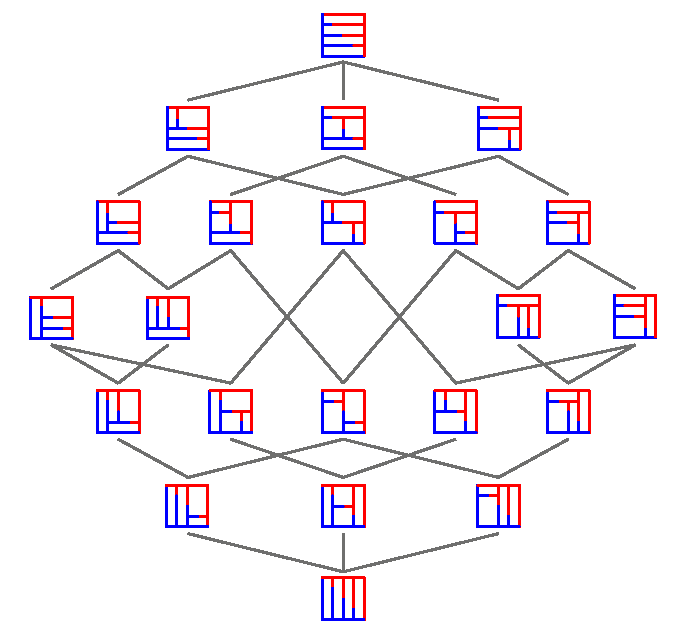
\includegraphics[scale=.9]{weakRectangulationLattice}}
	\caption{The weak rectangulation lattice.}
	\label{fig:weakRectangulationLattice}
\end{figure}

\begin{figure}
	\centerline{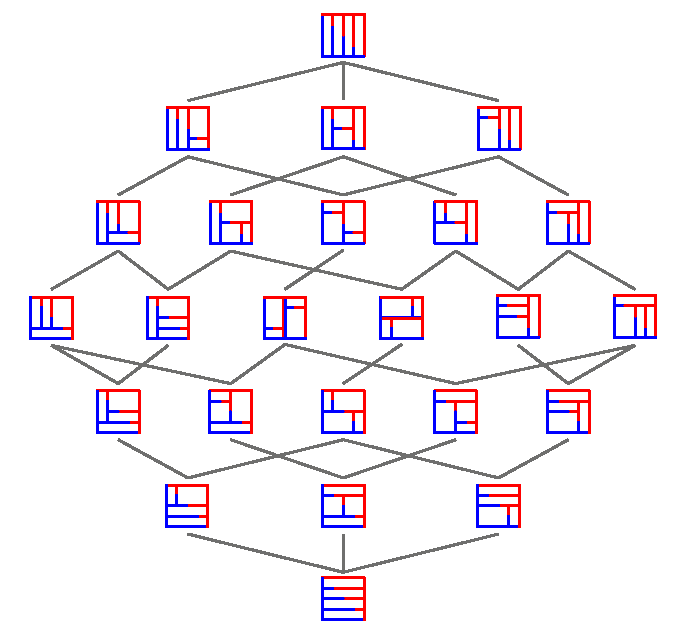
\includegraphics[scale=.9]{strongRectangulationLattice}}
	\caption{The strong rectangulation lattice.}
	\label{fig:strongRectangulationLattice}
\end{figure}

\end{document}
